\documentclass[11pt, twoside, openright, a4paper, chapterprefix]{scrbook}
\usepackage[inner=2.5cm, outer=2.5cm, top=4cm, bottom=4cm]{geometry}

%%% PACKAGES %%%%%%%%%%%%%%%%%%%%%%%%%%%%%%%%%%%%%%%%%%%%%%%%%%%%%%%%%%%%%%%%%%
%%%%%%%%%%%%%%%%%%%%%%%%%%%%%%%%%%%%%%%%%%%%%%%%%%%%%%%%%%%%%%%%%%%%%%%%%%%%%%%
%%
%%          $Id: packages.tex 385 2013-02-12 21:53:10Z holz $
%%    author(s): RoboCupAtWork Technical Committee(s)
%%  description: List of packages for the RoboCupAtWork rulebook
%%
%%%%%%%%%%%%%%%%%%%%%%%%%%%%%%%%%%%%%%%%%%%%%%%%%%%%%%%%%%%%%%%%%%%%%%%%%%%%%%%
\usepackage{soul}

\usepackage[english]{babel}
\usepackage{amsmath,amssymb,amsfonts}
\usepackage[nice]{nicefrac}
\usepackage{siunitx}
\usepackage{graphicx}
\usepackage{multicol}
\usepackage{verbatim}
\usepackage{fancyhdr}
% \usepackage{svn-multi}
\usepackage{color}
\usepackage{xcolor,colortbl}
\usepackage{epsfig}
\usepackage{makeidx}
\usepackage{lscape}
\usepackage{pdflscape}
\usepackage{picinpar}
% \usepackage{./styles/bar}
\usepackage{./styles/tweaklist}
\usepackage{subfig}
\usepackage{enumerate,paralist}
\usepackage{multirow}
\usepackage{pgffor}
\usepackage{array}
\usepackage{etoolbox}
\usepackage{hyperref}
\usepackage{tabularx}
\usepackage{xspace}
\usepackage[colorinlistoftodos]{todonotes}

%\usepackage[utf8x]{inputenc}
%\usepackage{times}
%\usepackage{helvet}
%\usepackage{courier}

\usepackage{url}
\usepackage{caption}
%\usepackage{subcaption}
\usepackage{epstopdf}
%\usepackage{subcaption}
\usepackage{float}
\usepackage{wrapfig}
%\usepackage{titlesec}
\usepackage{xfrac}

\usepackage[normalem]{ulem}  % used for \revadd, \revdel, etc.
\usepackage{xspace}  % used for adding spaces to macros, e.g. \RC, \RCAW, etc.
\usepackage[export]{adjustbox}  % used for valign option on images

\usepackage{pgfplots}
\usepgfplotslibrary{polar}

% Local Variables:
% TeX-master: "../Rulebook"
% End:

\usepackage[titletoc]{appendix}
\usepackage{enumitem}
\usepackage{mathtools}
\usepackage{gensymb}
\usepackage[normalem]{ulem}
\setlist{noitemsep}
\usepackage{hhline}
\usepackage{rotating}
\usepackage{tikz}
\usepackage{siunitx} %to have a nicer unit representation
\usepackage{multicol}
\usepackage{comment}

% Comment these both out for serif font
\usepackage{lmodern}
\renewcommand\familydefault{\sfdefault}

% Glossary
\usepackage[numberedsection, nogroupskip, nonumberlist, nopostdot]{glossaries}
\makeglossaries
\newglossaryentry{Manipulator}
{
	name=Manipulator,
	description={Manipulator is defined as the combination of arm and gripper.}
}
\newglossaryentry{Arm}
{
	name=Arm,
	description={Arm is defined as only the robot arm without the gripper.}
}
\newglossaryentry{Gripper}
{
	name=Gripper,
	description={Gripper is defined as only the gripper without the arm.}
}
\newglossaryentry{OC}
{
	name=OC,
	description={Organization Committee}
}
\newglossaryentry{TC}
{
	name=TC,
	description={Technical Committee}
}
\newglossaryentry{EC}
{
	name=EC,
	description={Executive Committee}
}
\newglossaryentry{TDP}
{
	name=TDP,
	description={Team Description Paper}
}
\newglossaryentry{START}
{
	name=START,
	description={START is defined as the area where the platform starts his run.}
}
\newglossaryentry{FINISH}
{
	name=FINISH,
	description={FINISH is defined as the area where the platform ends his run.}
}
\newglossaryentry{Wall}
{
	name=Wall,
	description={Wall is defined as physical wall in the arena and is static for the whole competition.}
}
\newglossaryentry{Obstacle}
{
	name=Obstacle,
	description={Obstacle is defined as a semi-static physical obstacle in the arena.}
}
\newglossaryentry{VirtualWall}
{
	name=Virtual Wall,
	description={Virtual Wall is defined as a static red/white Tape in the arena and is static for the whole competition.}
}
\newglossaryentry{VirtualObstacle}
{
	name=Virtual Obstacle,
	description={Virtual Obstacle is defined as a semi-static yellow/black Tape in the arena.}
}
\newglossaryentry{ServiceArea}
{
	name=Service Area,
	description={Service Area is defined as an area where the robot has to perform tasks. This can be at a Table, Rotating Table, Shelf or Precision Placement Table.}
}
\newglossaryentry{Container}
{
	name=Container,
	description={Container is defined as a red or blue industrial plastic stacking boxe with the size 2B }
}
\newglossaryentry{ManipulationZone}
{
	name=Manipulation Zone,
	description={Manipulation Zone is defined as the area at a Service Area in which the Objects has to be grasped or placed by the robot.}
}
\newglossaryentry{ArbitrarySurface}
{
	name=Arbitrary Surface,
	description={Arbitrary Surface is defined as an surface that has not the standard white color. Examples are wood pattern, grass, alufoil etc.}
}
\newglossaryentry{Decoy}
{
	name=Decoy,
	description={Decoy is defined as an Object that don't belong to the standard Objects.}
}
\newglossaryentry{Object}
{
	name=Object,
	description={Object is defined as a standard object that has to be grasped or placed by the robot.}
}
\newglossaryentry{Parcferme}
{
	name=Parc ferme,
	description={Parc ferme is defined as...}
}
\newglossaryentry{RefereeBox}
{
	name=Referee Box,
	description={Referee Box is defined as...}
}






\usetikzlibrary{arrows}
\usetikzlibrary{calc}
\usetikzlibrary{fit}
\usetikzlibrary{decorations.pathreplacing}
%%% SubfigureSetup %%%%%%%%%%%%%%%%%%%%%%%%%%%%%%%%%%%%%%%%%%%%%%%%%%%%%%%%%%%%
%\renewcommand{\subfigtopskip}{5pt}        % default is 10pt
%\renewcommand{\subfigbottomskip}{5pt}     % default is 10pt
%\renewcommand{\subfigcapskip}{3pt}        % default is 10pt
%\renewcommand{\subfigcapmargin}{7pt}      % default is 10pt

%%% TweakList-Setup %%%%%%%%%%%%%%%%%%%%%%%%%%%%%%%%%%%%%%%%%%%%%%%%%%%%%%%%%%%
\renewcommand{\itemhook}{%                 % modify itemize-spacing
  \setlength{\topsep}{2pt}%
  \setlength{\partopsep}{1pt}%
  \setlength{\itemsep}{-1pt}%
}
\renewcommand{\enumhook}{%                 % modify enumerate-spacing
  \setlength{\topsep}{2pt}%
  \setlength{\partopsep}{1pt}%
  \setlength{\itemsep}{-1pt}%
}
\renewcommand{\descripthook}{%             % modify description-spacing
  \setlength{\topsep}{2pt}%
  \setlength{\partopsep}{1pt}%
  \setlength{\itemsep}{-1pt}%
}

\setkomafont{title}{\normalfont}
\setkomafont{sectioning}{\normalfont\bfseries}
\addtokomafont{caption}{\small}
\setkomafont{captionlabel}{\small\bfseries}
\setkomafont{descriptionlabel}{\normalfont\bfseries}
\renewcommand*{\chapterformat}{\LARGE{Chapter \thechapter}}

\setcounter{secnumdepth}{3}

\setlength{\parskip}{10pt plus 1pt minus 1pt}
\setlength{\parindent}{0pt}

%%% MACROS %%%%%%%%%%%%%%%%%%%%%%%%%%%%%%%%%%%%%%%%%%%%%%%%%%%%%%%%%%%%%%%%%%%%
\newcommand{\YEAR}{2024\xspace}
\newcommand{\STATE}{Release 1.0}

%%%%%%%%%%%%%%%%%%%%%%%%%%%%%%%%%%%%%%%%%%%%%%%%%%%%%%%%%%%%%%%%%%%%%%%%%%%%%%%
%%
%%          $Id: macros.tex 399 2013-02-14 20:24:02Z holz $
%%    author(s): RoboCupAtHome Technical Committee(s)
%%  description: Macros for the RoboCupAtWork rulebook
%%
%%%%%%%%%%%%%%%%%%%%%%%%%%%%%%%%%%%%%%%%%%%%%%%%%%%%%%%%%%%%%%%%%%%%%%%%%%%%%%%

%%%%%%%%%%%%%%%%%%%%%%%%%%%%%%%%%%%%%%%%%%%%%%%%%%%%%%%%%%%%%%%%%%%% 
% Macros for generating score sheets for RoboCup@Work              %
% to be used in the rulebook or during the competition             %
%                                                                  % 
% Author: Dirk Holz & David Gossow                                 %
% Modif : Mauricio Matamoros                                       %
% $Id: macros_score_sheets.tex 429 2013-04-30 10:09:55Z holz $     %
%%%%%%%%%%%%%%%%%%%%%%%%%%%%%%%%%%%%%%%%%%%%%%%%%%%%%%%%%%%%%%%%%%%% 


\usepackage{calc}
\usepackage{ifthen}
\usepackage{wasysym}
\usepackage{chngpage}


%%% Counters / temp. variables %%%%%%%%%%%%%%%%%

\newcounter{currTestScore}
\newcounter{currTestScoreTotal}
\newcounter{currTestScoreTotalWithoutBonus}
\newcounter{currOutstandingBonus}
\newcommand{\scorelistOptions}{}
\newcommand{\scoresheetOptions}{}

% set \shortScoresheet to true for the rulebook version and to false for the referee's scoresheet
\newcommand{\shortScoresheet}{true}

% set \threeAttempts to true for three columns in the scoresheet
\newcommand{\threeAttempts}{false}

% set \retryAvailable to true for a second column in the scoresheet
\newcommand{\retryAvailable}{true}

% set \continueAvailable to true for CONTINUE sections
\newcommand{\continueAvailable}{true}

% name of the current test, is set automatically in the rulebook
\newcommand{\currentTest}{}

% (internal) if-clause shortcut to switch between short rulebook version and full score sheet for referees
\newcommand{\ifShortScoresheet}[2]{%
  \ifthenelse{ \equal{\shortScoresheet}{true}}{%
    #1%
  }{%
    #2%
  }%
}

\newcommand{\ifEvaluationSheet}[2]{%
  \ifthenelse{ \equal{\scoresheetOptions}{evaluationSheet}}{%
    #1%
  }{%
    #2%
  }%
}

% (internal) draws the scoresheet line for score handwritting
\newcommand{\scoreline}[1][0.08]{\rule{#1\linewidth}{.2pt}}

% (internal) draws the lines for score hadndwritting in the table outline based on the number of attempts
\newcommand{\attemptScoreLines}{
  \switchAttempts
    {\scoreline[0.06] & \scoreline[0.06] & \scoreline[0.06]}
    {\scoreline & \scoreline}
    {\scoreline}
}

% (internal) Select one of the provided arguments based on the number of attempts
% (3 tries, retry (2) or only try (1))
\newcommand{\switchAttempts}[3]{
  \ifthenelse{\equal{\threeAttempts}{true}}{#1}{\ifthenelse{\equal{\retryAvailable}{true}}{#2}{#3}}
}

% (internal) stores the number of attempts to perform
\edef\numAttempts{0}
% (internal) writes on the command \numAttempts the number of attempts to perform
\newcommand\defNumAttempts{
  \switchAttempts
  {\global\edef\numAttempts{3}}
  {\global\edef\numAttempts{2}}
  {\global\edef\numAttempts{1}}
}

%% commands for overriding internal calculations %%%%%%%%%%%%%%%%%%%%%%%%%%%%%%%%%%%%%%%%

% set score counter to arbitrary value
\newcommand{\setTotalScore}[1]%
{%
  \setcounter{currTestScore}{#1}
}

% set outstanding bonus to arbitrary value
\newcommand{\setOutstandingBonus}[1]%
{%
  \setcounter{currOutstandingBonus}{#1}
}




%% Score sheet page layout %%%%%%%%%%%%%%%%%%%%%%%%%%%%%%%%%%%%%%%%%%%%%%%%%%%%%%%%%%%%%%%%

% usage: \begin{scoresheet}[repeatable] ... \end{scoresheet}
\newenvironment{scoresheet}[1][]{
  % begin
  \newpage

  \renewcommand{\scoresheetOptions}{#1}
  
  \begin{minipage}[t]{0.8\textwidth}%
    \vspace{0pt}
    {\huge \textbf{Score Sheet} }
    
    \vspace{2 em}
    
    \begin{tabular}{ @{} l l l}
      \textbf{Test:} & \currentTest \\[.9 em]
      
      \ifEvaluationSheet{}{%
        \textbf{Team name:} & \scoreline[0.6]\\[.9 em]%
      }%
      % 
      \textbf{Referee name:} & \scoreline[0.6]\\[.9 em]%
      %	
      %	\ifEvaluationSheet{}{%
      %   \textbf{Restart:} & \Square ~1st try \hspace{1 em} \Square ~2nd try
      %	}
      %	
      % test repetition checkboxes (for stage 2 tests)
      \ifthenelse{ \equal{#1}{repeatable} }{%
	\textbf{Test repetition:} & \Square ~1st \hspace{1 em} \Square ~2nd\\[.9em]%
      }{}
    \end{tabular}

    \vspace{0.5 em}

  \end{minipage}
  \hfill
  \begin{minipage}[t]{0.15\textwidth}%
    \vspace{0pt}
    \includegraphics[width=\textwidth]{images/logo_RoboCupAtHome.jpg}%
  \end{minipage}\\
}
{
  % end
  \vspace{.2 em}
  \textbf{Remarks:}

  %% signatures of referee / team leader %%%%%%%%%%%%
  \vfill
  \ifEvaluationSheet{
    % team evaluation sheet
    \begin{tabular}{@{} @{\extracolsep{\fill}} l l @{}}
      \scoreline[0.25] \hspace{0.05\linewidth} & \scoreline[0.25] \hspace{0.05\linewidth}
      \\
      \textit{Date \& time}%
      & \textit{Referee}
    \end{tabular}
  }{
    % normal sheet
    \begin{tabular}{@{} @{\extracolsep{\fill}} l l l @{}}
      \scoreline[0.25] \hspace{0.05\linewidth} & \scoreline[0.25] \hspace{0.05\linewidth} & \scoreline[0.25]
      \\
      \textit{Date \& time}%
      & \textit{Referee} %
      & \textit{Team leader}
    \end{tabular}
  }

  \newpage
}


%% Score list table %%%%%%%%%%%%%%%%%%%%%%%%%%%%%%%%%%%%%%%%%%%%%%%%%%%%%%%%%%%%%%%%

% usage: \begin{scorelist}[openDoorSignal] ... \end{scorelist}
\newenvironment{scorelist}[1][]{
  % begin

  % init variables %%%%%%%%%
  \renewcommand{\scorelistOptions}{#1}
  \setcounter{currTestScore}{0}
  \setcounter{currOutstandingBonus}{0}

  % setup table %%%%%%%%%
  \vspace{0.8 em}

  \ifShortScoresheet {
    \begin{tabular*}{\textwidth}{@{} @{\extracolsep{\fill}} p{0.8\linewidth} r @{}}
      \ifEvaluationSheet{
        \textbf{Team} & \textbf{Score} \\ \hline 
      }{%
        \textbf{Action} & \textbf{Score} \\ \hline 
      }
    }{  
      % else:
      % \begin{tabular*}{\textwidth}{@{}p{0.65\linewidth}lp{0.15\linewidth}@{}}
      %   \textbf{Action} & \textbf{Score} & \multicolumn{1}{l}{\textbf{Success}}\\ \hline 
      \ifEvaluationSheet{
        \begin{tabular*}{\textwidth}{@{} @{\extracolsep{\fill}} p{0.7\linewidth} r r @{}}
          \textbf{Team} & \textbf{Score} & \textbf{Result}\\ \hline 
        }{
          \ifthenelse{\equal{\threeAttempts}{true}}{
            \begin{tabular*}{\textwidth}{@{} @{\extracolsep{\fill}} p{0.6\linewidth} r r r r @{}}
            \textbf{Action} & \textbf{Score} & \textbf{\small $1^{st}$ try} & \textbf{\small $2^{nd}$ try} & \textbf{\small$3^{rd}$ try} \\ \hline 
          }
          %else
          {
            \begin{tabular*}{\textwidth}{@{} @{\extracolsep{\fill}} p{0.6\linewidth} r r r @{}}
            \textbf{Action} & \textbf{Score} \ifthenelse{\equal{\retryAvailable}{true}}{& \textbf{1st try} & \textbf{2nd try}}{ & \textbf{Only try}} \\ \hline 
          }
        }
      }
    }
      {
        % end

	\ifEvaluationSheet{}{%
          
          % calculate max. score, outstanding bonus %%%%%%%
          \ifthenelse{\value{currOutstandingBonus} = 0}{%
            \setcounter{currOutstandingBonus}{ \value{currTestScore} / 10 }
          }{}
          \setcounter{currTestScoreTotal}{ \value{currTestScore} + \value{currOutstandingBonus} }
          \setcounter{currTestScoreTotalWithoutBonus}{ \value{currTestScore} }
          

          % Special penalties & bonuses %%%%%%%%%%%%%%%%
          \scoreheading{Special penalties \& bonuses}
          \ifShortScoresheet{}{
          	\ifthenelse {\equal{\continueAvailable}{true}}{\scoreitem[0.75]{0}{1st CONTINUE}}{}
          
          	\ifthenelse {\equal{\continueAvailable}{true}}{\scoreitem[0.50]{0}{2nd CONTINUE}}{}
		  }
          
          \scoreitem{-50}{Not attending \ifShortScoresheet{(see sec.~\ref{rule:not_attending})}{}}
          
          \ifthenelse{\equal{\scorelistOptions}{openDoorSignal}}{
            \scoreitem{-10}{Using start button \ifShortScoresheet{(see sec.~\ref{rule:start_button})}{}}
          }{}

          % \ifthenelse{\value{currOutstandingBonus} = 0}{
          \scoreitem{\thecurrOutstandingBonus}{Outstanding performance \ifShortScoresheet{(see sec.~\ref{rule:outstanding_performance})}{}}
          % }{}
          
          % Total score %%%%%%%%%%%%%%%%
          \hline\\
          % \textbf{Total score} & \scoring{ \thecurrTestScoreTotal } %
          \ifShortScoresheet {%
            % No Score per try in short version
          }{%
            \textbf{\textit{Score per try}} & \scoring{ \thecurrTestScoreTotalWithoutBonus } %
          }
          % add line to put in total:
          \ifShortScoresheet{}{& \attemptScoreLines} \\   
          \ifShortScoresheet{
            \textbf{Total score} (excluding penalties and bonuses) & \scoring{ \thecurrTestScoreTotalWithoutBonus } %
          }{
            \defNumAttempts
            & \\
            \textbf{Total score}  & \scoring{ \thecurrTestScoreTotalWithoutBonus } & \multicolumn{\numAttempts}{c}{\scoreline[0.20]}
          } \\
	}

      \end{tabular*}
      
    }


    %% Score sheet table entries %%%%%%%%%%%%%%%%%%%%%%%%%%%%%%%%%%%%%%%%%%%%%%%%%%%%%%%%%%%%%%%%

    % for loop helper
    % usage: \forloop[step]{counter}{initial_value}{conditional}{code_block} 
    \newcommand{\forloop}[5][1]%
    {%
      \setcounter{#2}{#3}%
      \ifthenelse{#4}%
      {%
 	#5%
 	\addtocounter{#2}{#1}%
 	\forloop[#1]{#2}{\value{#2}}{#4}{#5}%
      }%
      % else
      {%
      }%
    }

    \newcounter{ct}

    % heading
    % usage: \scoreheading{text}
    \newcommand{\scoreheading}[1]{
      \ifShortScoresheet {%
        \phantom{.} \\[-4 ex] \multicolumn{2}{@{}l}{\textbf{\textit{#1}}}\\[0pt]
      }{%
        \phantom{.} \\[-4 ex] \multicolumn{3}{@{}l}{\textbf{\textit{#1}}}\\[0pt]
      }
    }

    % table entry
    % usage: \scoreitem[multiplicity]{points}{description}
    \newcommand{\scoreitem}[3][1]{

      % add to max. total score if points > 0
      \ifthenelse{ #2 > 0 }{
        \addtocounter{currTestScore}{ #2 * #1 }
      }{}%
      % 
      \begin{minipage}[t]{\linewidth} {#3} \vspace{0.1 em} \end{minipage} & %
      \scoring{ \ifthenelse{ \equal{#1}{1} }{}{ #1 $\times$} \ifthenelse{ \equal{#2}{0} }{}{ #2}}%
      % insert check marks:	
      %	\ifShortScoresheet{}{ & \forloop{ct}{0}{\value{ct} < #1}{ \Square}} \\[3pt]
      % insert line
      \ifShortScoresheet{ %
        \\ 
      }{ % else
        \ifEvaluationSheet{}{& \attemptScoreLines} \\[0pt]
      }
    }


% Local Variables:
% TeX-master: "../Rulebook"
% End:

%%%%%%%%%%%%%%%%%%%%%%%%%%%%%%%%%%%%%%%%%%%%%%%%%%%%%%%%%%%%%%%%%%%%%%%%%%%%%%%
%%
%%          $Id: macros_open_demonstrations.tex 391 2013-02-14 07:57:07Z sugiura $
%%    author(s): holz
%%  description: simple macros for specifications of open challenges
%%
%%%%%%%%%%%%%%%%%%%%%%%%%%%%%%%%%%%%%%%%%%%%%%%%%%%%%%%%%%%%%%%%%%%%%%%%%%%%%%%

\newcommand{\OpenDemonstrationTask}[2] {
  \begin{enumerate}%
    \item \textbf{Setup and demonstration:} The team has a maximum of \timing{#1 minutes} for setup, presentation and demonstration.%
    \item \textbf{Interview and cleanup:} After the demonstration, there is
	      another \timing{#2 minutes} where the team answers %
    questions by the jury members.\\%
    During the interview time, the team has to undo its changes to the environment.%
  \end{enumerate}%
}

\newcommand{\OpenDemonstrationChanges}{
  \subsection{Changes to the environment}
  \begin{enumerate}
    \item \textbf{Making changes:} As in the other open demonstrations, teams are allowed to make modifications to the arena as they like, 
    but under the condition that they are reversible.
    \item \textbf{Undoing changes:} In the interview and cleanup team, changes need to be made undone by the team. 
    The team has to leave the arena in the \emph{very same} condition they entered it.
  \end{enumerate}
}
% Local Variables:
% TeX-master: "../Rulebook"
% End:


\newcommand{\rulebookVersion}{\STATE\ version for RoboCup \YEAR}

\def\RC{RoboCup\xspace}
\def\RCAW{RoboCup@Work\xspace}

\renewcommand{\labelenumi}{\arabic{enumi}.}
\renewcommand{\labelenumii}{\labelenumi\arabic{enumii}.}
\renewcommand{\labelenumiii}{\labelenumii.\arabic{enumiii}.}


%% %%%%%%%%%%%%%%%%%%%%%%%%%%%%%%%%%%%%%%%%%%%%%%%%%%%%%%%%% %%
%%                    Developement-Tools                     %%
%% %%%%%%%%%%%%%%%%%%%%%%%%%%%%%%%%%%%%%%%%%%%%%%%%%%%%%%%%% %%

%% %%%%%%%%%%%%%%%%%%%%%%%%%%%%%%%%%%%%%%%
\newcommand{\tbc}[1]{\textbf{\it\color{red}{t.b.c. ...}#1\color{black}}}
\newcommand{\chk}[1]{\textbf{\color{red}#1\color{black}}}

\newcommand{\revadd}[1]{\textcolor{blue}{#1}}
\newcommand{\revdel}[1]{\textcolor{red}{\sout{#1}}}
\newcommand{\revcha}[2]{\revdel{#1}\revadd{#2}}

\newcommand{\reworkon}{\marginpar{\raggedright\color{red}{$\downarrow$rework}\color{black}}}
\newcommand{\reworkoff}{\marginpar{\raggedright\color{red}{$\uparrow$rework}\color{black}}}

%% %%%%%%%%%%%%%%%%%%%%%%%%%%%%%%%%%%%%%%%
%%  site notes/margin notes
\def\note#1{\marginpar{\raggedright\tiny\color{blue}#1}}
\def\mpar#1{\marginpar{\raggedright\tiny#1}}
\def\rand#1{\marginpar{\raggedright\tiny#1}}
\setlength{\marginparwidth}{2cm}

\newcommand{\refsec}[1]{Section~\ref{#1}}
\newcommand{\reftab}[1]{Table~\ref{#1}}
\newcommand{\reffig}[1]{Figure~\ref{#1}}

%% %%%%%%%%%%%%%%%%%%%%%%%%%%%%%%%%%%%%%%%
%% side-annotation-macros for easy lookup
% \newcommand{\awardmark}{\marginpar{\centering\includegraphics[width=.34cm]{images/icon_award.pdf}}}
% \newcommand{\refmark}{\marginpar{\centering\includegraphics[width=.5cm]{images/icon_whistle.pdf}}}
% \newcommand{\referee}[1]{\emph{#1}\marginpar{\centering\includegraphics[width=.5cm]{images/icon_whistle.pdf}}}
% \newcommand{\scoremark}{\marginpar{\centering\includegraphics[width=.34cm]{images/icon_score.pdf}}}
\newcommand{\awardmark}{}
\newcommand{\refmark}{}
\newcommand{\referee}[1]{}
\newcommand{\scoremark}{}
%\newcommand{\scoring}[1]{\emph{#1}\marginpar{\centering\includegraphics[width=.34cm]{images/icon_score.pdf}}}
\newcommand{\scoring}[1]{\emph{#1}}
\newcommand{\timark}{\marginpar{\centering\includegraphics[width=.34cm]{icon_clock.pdf}}}

%\newcommand{\timing}[1]{\emph{#1}\marginpar{\centering\includegraphics[width=.34cm]{images/icon_clock.pdf}}}
\newcommand{\timing}[1]{\emph{#1}}

\def\svnRevision{Unknown} %
\def\svnChangeData{Unknown} %
\def\revnumtmpfile{.temp_rulebook_version}
\def\revdattmpfile{.temp_rulebook_date}
\immediate\write18{git rev-list HEAD | wc -l > \revnumtmpfile}
%\immediate\write18{svnversion . > \revnumtmpfile}
\IfFileExists{\revnumtmpfile}{\def\svnRevision{\input{\revnumtmpfile}\unskip}}{}
\immediate\write18{git log -1 --date=short  | grep 'Date:' | awk '{print $2}'> \revdattmpfile}
%\immediate\write18{svn info | grep 'Last Changed Date:' | awk '{print $4}'> \revdattmpfile}
\IfFileExists{\revdattmpfile}{\def\svnChangeData{\input{\revdattmpfile}\unskip}}{}
% \IfFileExists{\revnumtmpfile}{\immediate\write18{rm -f \revnumtmpfile}}{}
% \IfFileExists{\revdattmpfile}{\immediate\write18{rm -f \revdattmpfile}}{}
\newcommand{\VERSION}{Revision \svnChangeData\_\svnRevision}


% Local Variables:
% TeX-master: "../Rulebook"
% End:

%% %%%%%%%%%%%%%%%%%%%%%%%%%%%%%%%%%%%%%%%%%%%%%%%%%%%%%%%%%%%%%%%%%%%%%%%%%%%
%%
%%          $Id: abbrevix.tex 373 2013-02-12 20:32:49Z holz $
%%    author(s): RoboCupAtWork Technical Committee(s)
%%  description: Abbreviations for the RoboCupAtWork RuleBook
%%
%% %%%%%%%%%%%%%%%%%%%%%%%%%%%%%%%%%%%%%%%%%%%%%%%%%%%%%%%%%%%%%%%%%%%%%%%%%%%

%% temp-variables %%%%%%%%%
\newlength{\adxtemp}
\newlength{\adxspace}
\setlength{\adxspace}{3cm}

%% %%%%%%%%%%%%%%%%%%%%%%%%%%%%%%%%%%%%%%%
%%  Commands to use this
%% %%%%%%%%%%%%%%%%%%%%%%%%%%%%%%%%%%%%%%%

%% \abb{abk}
%% to reference an abbreviation
\newcommand{\abb}[1]{\hypertarget{#1}{#1}}

%% \term{the term}
%% print 'the term' in italic,
%% do not include 'the term' in index
%\newcommand{\term}[1]{#1\index{#1}}
\newcommand{\term}[1]{\textit{#1}}

%% \iterm{the term}
%% print 'the term' in italic,
%% include 'the term' in index
\newcommand{\iterm}[1]{\textit{#1}\index{#1}}

%% \nterm{the term}
%% do NOT print 'the term' but include 'the term' in index
\newcommand{\nterm}[1]{\index{#1}}

%% \TERM
%% print first term, add second term to index
\newcommand{\Term}[2]{\textit{#1}\index{#2}}


%% \aterm{the term}{abb}
%% print 'term', 
%% include 'term' with abbreviation 'abb' in abbreviation-index
\newcommand{\aterm}[2]{\settowidth{\adxtemp}{#2}{\hypertarget{#2}{#1 (#2)}\abbex{#2\hspace{\adxspace}\hspace{-\the\adxtemp}#1}}}

%% \iaterm{the term}{abbreviation} 
%% print 'term', 
%% include 'the term' in index, 
%% and include abbreviation in abbreviation-index
\newcommand{\iaterm}[2]{\settowidth{\adxtemp}{#2}{\hypertarget{#1}{\textit{#1} (#2)}\index{#1}\abbex{#2\hspace{\adxspace}\hspace{-\the\adxtemp}#1}}}

%% %%%%%%%%%%%%%%%%%%%%%%%%%%%%%%%%%%%%%%%
%%  Main Abbreviation Definitions
%% %%%%%%%%%%%%%%%%%%%%%%%%%%%%%%%%%%%%%%%

\makeatletter
\newlength{\QZ@TOChdent}% Used to define hanging indents.
\setlength{\QZ@TOChdent}{1.0em}%
\renewcommand{\@pnumwidth}{1.55em}%
\makeatother
%
%\newenvironment{simpleenv}[4]{\clearpage}{\clearpage}%
%\newenvironment{simpleenv}[4]{\clearpage}{\pagebreak}%
\newenvironment{simpleenv}[4]{\pagebreak}{\pagebreak}%
\newcommand{\BaseDiff}{0}%
%\newcommand{\RSpnum}[1]{\makebox[\@pnumwidth][r]{#1}}%
\newcommand{\RSpnum}[1]{\makebox[1.57em][r]{#1}}%
\newcommand{\RSnopnum}[1]{\makebox[\@pnumwidth][r]{}}%
\newcommand{\RSpset}[1]{\RSpnum{#1}}%
%
\newcommand{\printabbex}[4][\jobname]{%
  \typeout{ ***** printabbex #1 #2 #3 #4 for file \jobname.tex}%
  \IfFileExists{#1.and}{%
     \begin{simpleenv}{#1}{#2}{#3}{#4}%
       \pagestyle{plain} %
       \addcontentsline{toc}{chapter}{#2}%
       \chapter*{\textbf{#3}}{#4}%
       \input{#1.and}%
       \vfill%
     \end{simpleenv}%
   }%
   {\typeout{ ***** ERROR: No file #1.and found for file \jobname.tex.}}}%
\renewcommand{\see}[2]{#2 \emph{see} #1}%
\makeatletter
\newcommand{\makeabbex}[1][\jobname]{\begingroup
  \makeatletter
  \if@filesw \expandafter\newwrite\csname #1@adxfile\endcsname
  \expandafter\immediate\openout \csname #1@adxfile\endcsname #1.adx\relax
  \typeout{ ***** Writing abbex file #1.adx for file \jobname.tex.}%
  \fi \endgroup}
%\makeatother
%\makeatletter
\@onlypreamble{\makeindex}%
\newcommand{\abbex}[2][\jobname]{\@bsphack\begingroup
               \def\protect##1{\string##1\space}\@sanitize
               \@wrabbex{#1}{#2}}
\newcommand{\@wrabbex}[2]{\let\thepage\relax
   \xdef\@gtempa{\@ifundefined{#1@adxfile}{}{\expandafter
      \write\csname #1@adxfile\endcsname{\string
      \indexentry{#2|}{\thepage}}}}\endgroup\@gtempa
   \if@nobreak \ifvmode\nobreak\fi\fi\@esphack}
\makeatother
\newcommand{\indxspace}{\par\vspace{\BaseDiff\baselineskip}}
\makeatletter
\newcommand{\IndexSet}{%
\renewcommand{\@idxitem}{\par\setlength{\leftskip}{0pt}%
                         \setlength{\hangindent}{\QZ@TOChdent}}%
\renewcommand{\subitem}{\par\setlength{\leftskip}{0.25in}%
                         \setlength{\hangindent}{\QZ@TOChdent}}%
\renewcommand{\subsubitem}{\par\setlength{\leftskip}{0.5in}%
                         \setlength{\hangindent}{\QZ@TOChdent}}%
\renewcommand{\indexspace}{}
\renewcommand{\indxspace}{\par\vspace{\BaseDiff\baselineskip}}
\renewenvironment{theindex}{%
                \setlength{\parindent}{\z@}%
                \parskip\z@ \@plus .3\p@\relax
                \setlength{\rightskip}{\@tocrmarg}%
                \setlength{\parfillskip}{-\rightskip}%
                \let\item\@idxitem}
} %% End of the IndexSet definition
\makeatother

\newcommand{\printidx}{\addcontentsline{toc}{chapter}{Index}\printindex}
\newcommand{\printabx}{\printabbex{Abbreviations}{Abbreviations}{}}
%\newcommand{\printabbrevidx}{\printindex[abb]{Abk�rzungen}{Abk�rzungen}{}}
\newcommand{\printabbrevidx}{\printabbex{Abbreviations}{Abbreviations}{}}
%\newcommand{\makeabbrevidx}{\makeindex[abb]}
\newcommand{\makeabbrevidx}{\makeabbex}

% Local Variables:
% TeX-master: "../Rulebook"
% End:


\makeindex                                % generate index
\makeabbex                                % generate abbreviations

%%% DOCUMENTINFO %%%%%%%%%%%%%%%%%%%%%%%%%%%%%%%%%%%%%%%%%%%%%%%%%%%%%%%%%%%%%%
\hypersetup{
  pdftitle     = {\RCAW Rulebook},
  pdfsubject   = {\RCAW Rulebook},
  pdfauthor    = {\RCAW Technical Committee},
  pdfkeywords  = {\RC, @Work, Rules, Competition},
  colorlinks   = true,
  anchorcolor  = blue,
  linkcolor    = blue,
  urlcolor     = blue,
}

%%% HEADINGS & PAGE STYLE %%%%%%%%%%%%%%%%%%%%%%%%%%%%%%%%%%%%%%%%%%%%%%%%%%%%%
\newcommand{\footline}{\RCAW Rulebook / \rulebookVersion}
\pagestyle{fancy}
\renewcommand{\chaptermark}[1]{\markboth{\chaptername\ \thechapter. \ #1}{}}
\renewcommand{\sectionmark}[1]{\markright{\thesection \ #1}{}\renewcommand{\currentTest}{#1}}
\fancyhf{}
\fancyhead[LE,RO]{\thepage}
\fancyhead[RE]{\sffamily\rightmark}
\fancyhead[LO]{\sffamily\leftmark}
\fancyfoot[C]{\scriptsize \sffamily \footline{}}
\fancypagestyle{plain}{
        \fancyhf{}
        \fancyhead[LE,RO]{\thepage}
        \fancyhead[RE]{\sffamily\rightmark}
        \fancyhead[LO]{\sffamily\leftmark}
        \fancyfoot[C]{\scriptsize \sffamily \footline{}}
		\renewcommand{\headrulewidth}{0.5 pt}
}
\fancypagestyle{empty}{
        \fancyhf{}
        \fancyhead{}
        \fancyfoot[C]{\scriptsize \sffamily \footline{}}
		\renewcommand{\headrulewidth}{0 pt}
}

\newcommand{\quotes}[1]{``#1''}
\newcommand{\textbi}[1]{\textbf{\textit{#1}}}
%\newcommand{\sectionbreak}{\clearpage}
%\newcommand{\subsectionbreak}{\clearpage}


%%%%%%%%%%%%%%%%%% Please add your personal makro here %%%%%%%%%%%%%%%%%%%%%%%%
\newcommand{\szug}[1]{\todo[color=green!40, inline, caption={}]{[Sebastian] #1}}
\newcommand{\marco}[1]{\todo[color=green!40, inline, caption={}]{[Marco     ] #1}}
\newcommand{\deebul}[1]{\todo[color=yellow!40, inline, caption={}]{[Deebul     ] #1}}
\newcommand{\christoph}[1]{\todo[color=teal!40, inline, caption={}]{[Christoph     ] #1}}
\newcommand{\martin}[1]{\todo[color=green!50, inline, caption={}]{[Martin          ] #1}}
\newcommand{\leander}[1]{\todo[color=orange!50, inline, caption={}]{[Leander          ] #1}}
\newcommand{\all}[1]{\todo[color=red!40, inline, caption={}]{[all     ] #1}}
\newcommand{\lucas}[1]{\todo[color=yellow!40, inline, caption={}]{[Lucas     ] #1}}

%%%%%%%%%%%%%%%%%%%\renewcommand{%%%%%%%%%%%%%%%%%%%%%%%%%%%%%%%%%%%%%%%%%%%%%%
%%%%%%%%%%%%%%%%%%%%%%%%%%%%%%%%%%%%%%%%%%%%%%%%%%%%%%%%%%%%%%%%%%%%%%%%%%%%%%%
%%%%%%%%%%%%%%%%%%%%%%%%%%%%%%%%%%%%%%%%%%%%%%%%%%%%%%%%%%%%%%%%%%%%%%%%%%%%%%%

\begin{document}
\errorcontextlines 10000
%\listoftodos
% !TEX root = ../Rulebook.tex

\begin{titlepage}
  \begin{center}
    {

      
\includegraphics[width=\textwidth]{images/logo_RoboCupAtWork.pdf}\\[1.23ex]
    }
    \vspace{2.7 cm}
    \hrulefill\par
    {%
      \vspace*{.27cm}
      \Huge{\RCAW}\\[1.23ex]
      \Large Rulebook \\[2ex]
    }

    \hrulefill\par

    \vfill
    Caleb Fook \\
    Marco Masannek\\
    Asad Norouzi\\
    Wiebke Outzen\\
    Lucas Reinhart\\
    Christoph Steup
    \vfill
    ~~ Version: \YEAR ~~ \\
    ~~  \today ~~ \\
    %\vfill
  \end{center}

\newpage

\section*{Acknowledgments}

We would like to thank to previous @Work members that supported the league and advanced the rulebook over years:
\begin{itemize}
\item Jan Carstensen 
\item Frederik Hegger
\item Nico Hochgeschwender 
\item Daniel Kaczor 
\item Robin Kammel 
\item Alexander Moriaty 
\item Walter Nowak 
\item Benjamin Schnieders
\item Armin Shahsavari 
\item Jon Martin 
\item Asadollah Norouzi
\item Sebastian Zug
\item Deebul Nair
\item Maximilian Hachen
\item Kenny Voo
\item Martin Sereinig
\item Leander Bartsch
\end{itemize}


Furthermore we would like to acknowledge the following people for contributing to the development
of the \RCAW league:

\begin{itemize}
	\item Gerhard Kraetzschmar
	\item Rainer Bischoff
	\item Daniel Kazcor
	\item Arne Hitzmann
	\item Frederik Hegger
	\item Herman Bruyninckx
	\item Sven Schneider
	\item Jakob Berghofer
\end{itemize}
In July 2019 our league lost one of the initiators and founding members. Prof. Dr. Gerhard
Kraetzschmar has been very active in many functions within the RoboCup-Community
for decades. We are grateful for his efforts, advises and motivation and will respect his memory.


\begin{minipage}{\textwidth}
\section*{How to cite the rulebook or \RCAW in general}
If you refer to the this rulebook in particular, please cite:

\begin{verbatim}
	@misc{rulebook_2024,
		author = {Caleb Fook, Marco Masannek, Asad Norouzi, Wiebke Outzen, Lucas Reinhart, Christoph Steup},
		title  = {RoboCup@Work 2024 - Rulebook},
		year   =  2024,
		howpublished = {\url{https://atwork.robocup.org/rules/}},
	}
\end{verbatim}


For the citation of the \RCAW please use:
\begin{verbatim}
	@InCollection{Kraetzschmar2014,
		Title = {RoboCup@Work: Competing for the Factory of the Future},
		Author = {Kraetzschmar, Gerhard K. and Hochgeschwender, Nico and Nowak, Walter
			and Hegger, Frederik and Schneider, Sven and Dwiputra, Rhama and Berghofer, Jakob
			and Bischoff, Rainer},
		Booktitle = {RoboCup 2014: Robot World Cup XVIII},
		Publisher = {Springer International Publishing},
		Year = {2015},
		Editor = {Bianchi, Reinaldo A. C. and Akin, H. Levent and
			Ramamoorthy, Subramanian and Sugiura, Komei},
		Pages = {171-182},
		Series = {Lecture Notes in Computer Science},
		Volume = {8992}
	}
\end{verbatim}
\end{minipage}




\end{titlepage}


\pagestyle{empty}
%\listoftodos[Todos, Discussions, Remarks]

\tableofcontents
\clearpage

\pagestyle{plain}

% !TEX root = ../Rulebook.tex

\chapter{Summary of Changes}

\begin{comment}
This chapter provides an overview for experienced teams that know the rules and just need an update on what is new for the specific year. 
All new teams are strongly advised to read the whole rule book thoroughly.
\end{comment}

\section{Season 2024}

For the Season 2024, we mainly added some clarifications regarding onsite events and the usage of ATTCs.

\subsection{Open Source Award}

We added an open source award which should encourage share of code and knowledge between teams with the intention to improve the league community and simplify the initial steps to participate (see \ref{sec: osa}).

\subsection{Clarifications}

We added some clarifications regarding:

\begin{itemize}
	\item Arbitrary Surfaces and objects sinking into them
	\item Default table size and allowed margin for onsite constructions
	\item Placing multiple objects into the same container
	\item The maximum size for decoy objects to avoid damage on manipulators
\end{itemize}

\subsection{Teamleader Meetings}

We added timeslots for teamleader meetings to the official onsite schedule.
They have always been part of onsite events but were a bit difficult to organize without official requirements 
with the recently increasing number of participating teams.

\subsection{April Tagged Object - Details}

We've added some detailed requirements for the usage of April Tagged Objects,
mainly targeting better usability and handling for onsite events.
We also removed some bonus points for manipulation of ATTCs as we felt that they were unjustified
considering the much lower technical hurdle.

To ensure that we can actually replace a regular task with the simplified ATT version,
teams wanting to use that option are required to provide two complete sets of prepared objects for onsite events.

\section{Season 2023}

\subsection{Restructuring of Benchmark Tests}

The specialized tasks Precise Placement and Rotating Table have been integrated into the new Advanced Transportation Tasks and the Final.
The standalone tests have therefore been removed from the competition schedule, effectively reducing the number of total tests by one.

\subsection{Linear Increase of Complexity}

The elements included in the different tests have been adjusted to form a more linear increase of overall task complexity over the course of the competition. This should allow teams to participate in the tests more successful for longer while still setting benchmarks in the advanced tests.

\subsection{Replacement of the RoCKIn Object Set with the new Advanced Set}

The objects from previous years technical challenge "Real Object Test" have been added to the new Advanced Object set. This replaces the outdated RoCKIn object set for this season and onwards.

\subsection{Introduction of April Tagged Objects}

With increasing requirements for object recognition due to the introduction of arbitrary surfaces and more difficult objects, the object detection is very critical for teams to being able to perform tasks in the league. To relax the initial boundary of this task, an option to replace the real objects with April tagged cubes has been introduced. Teams can then focus on other aspects of the league (navigation, task optimization, etc.) while being able to participate in the league successfully. As the final benchmark still foresees actual detection and recognition of real objects, a penalty is applied when a team uses this simplification.

\subsection{Clarifications for successful manipulation}

Some unclear situations were adressed with some clarifications regarding successful object placement on the table, in containers and on precise placement tiles.

\subsection{Referee Briefing}

An additional organization slot was added to the schedule that shall be used to brief the referees of each team for the upcoming competition tests. Only briefed refs are allowed to judge the future runs.
Teams are asked to send at least two members to the briefing, if possible.

\subsection{Minimum Ref Number}

A lower boundary of 4 for the amount of refs required for "fair" judgement was added.
In case of only a few attending teams and therefore lower referee numbers,
TC members will assist in the judging process.

\subsection{Technical Challenges}

The technical challenge "Real Object Test" has been removed as the new object set is used in the benchmark tests.



\section{Season 2022}

\subsection{General Changes for 2022}

In 2021, the first virtual robocup was held online via discord, zoom and youtube live.
As a lot of new teams came into the league which never experienced a in-person robocup,
it came clear that the rulebook was missing out on specific information and rule definitions.
A lot of the rules have been habit and spoken agreements during the years,
which included crucial elements such as handling of robot collisions, repeating runs,
on-site competition organization and more.

This years rulebook tries to clarify all these rules, while also releasing some constraints 
while enforcing more robot safety. In the following, 
some rule summaries are being made about the following chapters.
Please carefully read the paragraphs anyways.

\subsection{Chapter 2: League Organization}

Discord has proven to be a very useful tool to organize 
robocups as it allows teams to communicate. All participating teams should join our Discord to keep up on news and announcements.

\subsection{Chapter 3: Robot Rules}

The size constraints were relaxed to allow more chassis types.
However, certain safety requirements must be met to participate in the competition.

\subsection{Chapter 3: Environment Specification}

The requirements for a robot to autonomously navigate the arena have been specified. Robots must fit those specs to participate.

The arena elements and their role in the competition are defined, declaring a task location a service area.
Robots must perform various manipulation tasks at service areas, mostly by handling a set of objects.



\subsection{Chapter 4: The Competition}

The on-site process is defined and explained, most importantly the rules and schedule of runs. Robots must autonomously perform a set of tasks at different service areas, where the exact task definition is defined by so called tests.

Each team has one performance slot for each test type (currently 7+1), with the option to repeat a lower-scoring test once in a later timeslot if possible.
A performance slot consists of a prep phase, a run phase and the end phase, where the performing team prepares and executes their run and then gets their performance then evaluated by the refs.

\subsection{Chapter 5: Test Definition}

Clarification of the basic manipulation, basic transportation, precise placement and rotating table test.


\subsection{Chapter 6: Scoring Adjustments}

The scoring for successful task execution and errors has been updated to ease the competition for newer teams while keeping the ambitions for more difficult tasks with boni.

\subsection{Chapter 7: Virtual Cups}

Taking the rules from 2021s virtual cup, 
requirements for arena setups at home are defined to allow teams to participate in their own laboratory.
They must livestream their test performance with a professional camera setup to allow refs worldwide to evaluate the performance.

\subsection{Chapter 8: Technical Challenges}

Three new technical challenges have been introduced to help evolve the league and the scientific challenges. 
The exact specification of the individual tests is yet to be made.
	


\chapter{Introduction}
\section{\RCAW in a Nutshell}\label{sec:at_work_nushell}
\RCAW is a competition in \RC that targets the use of robots in work-related scenarios. \RCAW utilizes proven ideas and concepts from \RC competitions to tackle open research challenges in industrial and service robotics. With the introduction of this new event, \RC opens up to communities researching both classical and innovative robotics scenarios with very high relevance for the robotics industry. 
\par
Examples for the work-related scenarios targeted by \RCAW include

\begin{itemize}
	\item loading and/or unloading of containers with/of objects with the same 	or different size,
	\item pickup or delivery of parts from/to structured storages and/or 				unstructured heaps,
	\item operation of machines, including pressing buttons, opening/closing 			doors and drawers, and similar operations with underspecified or unknown 			kinematics,
	\item flexible planning and dynamic scheduling of production processes 			involving multiple agents (humans, robots, and machines),
	\item cooperative assembly of non-trivial objects, with other robots 				and/or humans,
	\item cooperative collection of objects over spatially widely  distributed 	areas, and
	\item cooperative transportation of objects (robots with robots, robots 			with humans).
\end{itemize}

The \RCAW scenarios target difficult, mostly unsolved problems in robotics, artificial intelligence, and advanced computer science, in particular in perception, path planning and motion planning, mobile manipulation, planning and scheduling, learning and adaptivity, and probabilistic modeling, to name just a few. Furthermore, \RCAW scenarios may also address problems for which solutions require the use and integration of semantic web technology, RFID technology, or advanced computational geometry.
\par

Solutions to the problems posed by \RCAW require sophisticated and innovative approaches and methods and their effective integration. The scenarios are defined such that the problems are sufficiently general and independent of particular industrial applications, but also sufficiently close to real application problems that the solutions can be adapted to particular application problems with reasonable effort.
\par

\clearpage

A \RCAW competition has only recently become a feasible idea for several reasons: The arrival of new, small, and flexible robot systems for mobile manipulation allow more university-based research labs to perform research in the above-mentioned areas. Advances and a revived interest in the use of simulation technology in robotics enable research groups to perform serious research without having a full set of costly robotics and automation equipment available.
\par

The robotics and automation industry is recently shifting its attention towards robotics scenarios involving the integration of mobility and manipulation, larger-scale integration of service robotics and industrial robotics, cohabitation of robots and humans, and cooperation of multiple robots and/or humans. Last but not least, there is a huge interest by funding agencies and professional societies in well-designed and professionally performed benchmarks for industry-relevant robotics tasks. \RCAW is designed as an instrument to serve all these needs.
\par


\section{Organization of the League}
\label{sec:organisation_of_the_league}

\subsection{League Committees}
The following list of committees is implemented for \RCAW.

\subsubsection{Executive Committee}

\iaterm{Executive Committee}{EC} members are responsible for the long term goals of the league and thus have also contact to other leagues as well as to the \RC Federation. The EC presents the league and its achievements to the \RC Federation every year and gets feedback to organize the league. All EC members are also members of the Technical Committee. EC members are elected by the Board of Trustees and appointed by the President of the \RC Federation, they serve 3-year terms. The current EC members are:

\begin{itemize}
	\item Asadollah Norouzi, \textit{Singapore Polytechnic}
    \item Christoph Steup, \textit{Otto von Guericke University Magdeburg}
\end{itemize}

\subsubsection{Technical Committee}
The \iaterm{Technical Committee}{TC} is responsible for technical issues of the league, most notably the definition of the rules, such as compliance of the robots with rules and safety standards, the qualification of teams, the adherence to the rules as well as the resolution of any conflicts that may arise during competition. The current TC members are:

\begin{itemize}
	\item Marco Masannek, \textit{Nuremberg Institute of Technology}
	\item Lucas Reinhart, \textit{University of Applied Sciences W{\"u}rzburg-Schweinfurt}
	\item Kenny Voo, \textit{Nanyang Technological University} 
	\item Martin Sereinig, \textit{University of Innsbruck} 
	\item Leander Bartsch, \textit{Otto von Guericke University Magdeburg} 
\end{itemize}

\subsubsection{Organizing Committee}
The \iaterm{Organizing Committee}{OC} is responsible for all aspects concerning the practical implementation of competition, most notably for providing the competition arenas, ensuring their conformity with the rules, and any objects and facilities required to perform the various tests. Further, the Committee is responsible for assigning space to teams in the team area, the organization and scheduling of meetings, the nomination and scheduling of referees, the scheduling and timely execution of tests and stages, recording and publishing competition results, and any other management duties arising before, during, and after a competition. The current OC members are:

\begin{itemize}
	\item Franziska Labitzke, \textit{Otto von Guericke University Magdeburg}
	\item Hauke Petersen, \textit{Otto von Guericke University Magdeburg} 
	\item Sally Zeitler, \textit{Nuremberg Institute of Technology}
\end{itemize}







%\subsubsection{Industrial Advisory Board}

%The role of the Industrial Advisory Board is to ensure the industrial relevance of the tests and the overall competition. It allows representatives from industry to voice interesting new problems, which may be included in existing or new test scenarios.
%\par
%Currently, the Industrial Advisory Board has no members yet.

%\subsubsection{ Research Advisory Board}

%The role of the Research Advisory Board is to ensure that the tests and scenarios are innovative and relevant from a research point of view. The members will be recruited from academic institutions and research organizations.
%\par
%Currently, the Research Advisory Board has no members yet.

\subsection{League Infrastructure}
\label{ssec:LeagueInfrastructure}

In order to provide a forum for continuous discussions between teams and other stakeholders, the league builds and maintains an infrastructure consisting of a web site, mailing lists, and repositories for documentation, software, and data. The infrastructure is complemented by a minimum infrastructure to be built and maintained by teams, i.e. teams should eventually create their own web page to which the \RCAW League's web pages can be linked.


\subsubsection{Infrastructure Maintained by the League} 

\paragraph{Website}
The official website of \RCAW is at
\begin{center}
\url{https://atwork.robocup.org/}.
\end{center}

This web site is the central place for information about the league. It contains general introductory information plus links to all other infrastructure components, such as a league wiki, the mailing lists, important documents such as this rule book, announcements of upcoming events as well as past events and participating teams.


\paragraph{Discord Server}
The official Discord server of \RCAW is
\begin{center}
	\href{Official Discord Server}{https://discord.gg/6jg7Yv49Dn}
\end{center}

Teams are asked to join the server, as it is a place for exchange in the league. 
Things as Questions, Announcements and Discussions are usually held here.

\paragraph{Mailing Lists}
The league maintains several mailing lists:

\texttt{rc-work@lists.robocup.org} this is the general \RCAW mailing list. Anyone can subscribe, but a real name must be provided either as part of the email address or being specified on the mailing list subscription page. The list is moderated in order to avoid abuse by spammers. New members can subscribe to this list here: 
	\begin{center}
		\url{https://lists.robocup.org/cgi-bin/mailman/listinfo/rc-work}.
	\end{center}

\texttt{rc-work-tc@lists.robocup.org} this is the mailing list for the TC. Posts from non-members have to be approved by the list moderator. Approvals will be given only in well-justified cases.
\begin{center}
\url{https://lists.robocup.org/cgi-bin/mailman/listinfo/rc-work-tc}
\end{center}



\paragraph{Repositories}
Several repositories are publicly available under the official \RCAW Github account:
\begin{center}
\url{https://github.com/robocup-at-work}
\end{center}

The repositories provide 3D models for the manipulation objects, their corresponding PPT cavities, and all arena elements. Additionally, the sources to this rulebook, the implementation of the referee box, and various tools can be found.


\paragraph{Team Description Paper Template}
All TDPs must be written using the following template:
\begin{center}
	\url{https://www.overleaf.com/latex/templates/springer-lecture-notes-in-computer-science/kzwwpvhwnvfj#.WtR5Hy5ua71}
\end{center}


\subsubsection{Infrastructure Maintained by Teams}
Each team is requested to build and maintain a minimum infrastructure for its team. This infrastructure consist of

\begin{itemize}
	\item team website,
	\item team contact, and
	\item team mailing address.
\end{itemize}

The team web site should contain the following information:

\begin{itemize}
	\item Name of the team, and team logo, if any
	\item Affiliation of the team
	\item Team leader including full contact information
	\item List of team members
	\item Description of the team's research interest and background
	\item Description of specific approach pursued by the team
	\item Description of the robot(s) used by the team
	\item List of relevant publications by team members

\end{itemize}

The team contact should be the official contact of the team. Usually, for university-based teams, this would be an academic person such as a professor or post-doc, who should, however, be responsive and be able to answer quickly when contacted by email.
\par
The team mailing address should be an email alias, which should be used to subscribe the team to the general \RCAW mailing list. The email alias should at least include the team contact and the team leader.

\section{Participation in the Competition}\label{sec:participation_in_the_competition}
Participation in \RCAW requires successfully passing a qualification procedure. This procedure is to ensure the quality of the competition event and the safety of participants. Depending on constraints imposed by a particular site or the number of teams interested to participate, it may not be possible to admit all interested teams to the competition.

%\todo[inline]{Needs to be reviewed by Execs}

\subsection{Steps to Participate}
All teams that intend to participate at the competition have to perform the following steps:

\begin{enumerate}
	\item Preregistration (may be optional; currently by sending email to the TC)
	\item Submission of qualification material, including a team description paper, a promotional videos and possibly additional material like designs or drawings
	\item Final registration (qualified teams only)
  \item Entering the competition
\end{enumerate}


All dates and concrete procedures will be communicated in due time in advance.

\subsection{Qualification}
The qualification process serves a dual purpose: It should allow the TC to assess the safety of the robots a team intents to bring to a competition, and it should allow to rank teams according to a set of evaluation criteria in order to select the most promising teams for a competition, if not all interested teams can be permitted. The TC will select the qualified teams according to the qualification material provided by the teams. The evaluation criteria will include:

\begin{itemize}

	\item Team description paper
	\item Relevant scientific contribution/publications
	\item Professional quality of robot and software
	\item Novelty of approach
	\item Relevance to industry
	\item Performance in previous competitions
	\item Contribution to \RCAW league, e.g. by
		\begin{itemize}
			\item Organization of events
			\item Provision and sharing of knowledge
		\end{itemize}
	\item Team promo video
	\item Team web site

\end{itemize}

\subsection{Team Description Paper}
The \iaterm{Team Description Paper}{TDP} is a central element of the qualification process and has to be provided by each team as part of the qualification process. All TDPs will be included in the CD proceedings of the \RC Symposium.
The TDP should at least contain the following information in the author/title section of the paper:

\begin{itemize}
	\item Name of the team (title)
	\item Team members (authors), including the team leader
	\item Link to the team web site
	\item Contact information
\end{itemize}


The body of the TDP should contain information on the following:

\begin{itemize}
	\item focus of research/research interest
	\item description of the hardware, including an image of the robot(s)
	\item description of the safety systems used on the robot, including emergency stop procedure
	\item description of the software, esp. the functional and software architectures
	\item innovative technology (if any)
	\item reusability of the system or parts thereof
	\item applicability and relevance to industrial tasks
\end{itemize}

The team description paper should cover in detail the technical and scientific approach, while the team web site should be designed for a broader audience. Both the web site and the TDP have to be written in English. Alongside the TDP, the TC will - starting 2019 - also require a video file presenting the robot, see Section~\ref{ssec:promotional_video}. All TDPs must be written using the following template: \href{https://www.overleaf.com/latex/templates/springer-lecture-notes-in-computer-science/kzwwpvhwnvfj#.WtR5Hy5ua71}{Overleaf TDP template} 

\subsection{Promotional Video}
\label{ssec:promotional_video}
In order to better judge the quality of a team's qualification, the TC asks every team, established or new, to submit a video file describing the robot and its design. The video should clearly demonstrate the robot's ability to perform the tasks required in the challenge, such as autonomous navigation, picking, and placing. Desired elements include visualizing the sensory capabilities of the robot, i.e., seeing what the robot sees, and the plan currently followed by the robot. Spoken language/an audio stream is not required. Ideal video resolution is 1080p with a 16:9 ratio. For large files, please provide a download link.
This file will also be played as explanatory and promotional material during the competiton.

\subsection{Contribution to On-Site Events}%
\label{sec:participation}
To actually participate in an on-site competition,
 teams must bring one set of all objects used in the competition. 
 
 This includes the Basic and Advanced Object Set, see Section~\ref{subsec:containers} and the
containers, see Section~\ref{ssec:ManipulationObjects}. The objects are used as part of the league's object pool, which are used to realize the official tasks generated by the Atwork Commmander, see Section~\ref{sec:atwork-commander}. 

Provision
of arbitrary surfaces, see Section~\ref{subsec:Arbitrary_Surfaces_and_Decoys} is optional, but highly appreciated to ensure a large variarity of
surfaces for the tasks. 

If teams want to make use of existing simplifications, they also need to provide the necessary
equipments for these. For more informations refer to Sections~\ref{ssec: April Tagged Object Set}~and~\ref{ssec:simplification_ato}.

%% !TEX root = ../Rulebook.tex

\section{Organization of the Competition}\label{sec:organization_of_the_competition}

\subsection{Teams}
The TC and OC will jointly determine the number of teams permitted to participate in a competition well in advance. The rules shall enable a competition with up to at least 24 teams lasting not more than four full days.
The number of people to register per team is not restricted by default, but may be limited due to local arrangements. Teams that plan to bring more than four members are advised to contact the OC beforehand.
During registration, each team has to designate one member as team leader. A change of the team leader must be communicated to the OC. The team leader is the only person who can officially communicate with the referees during a run, e.g. to decide to abort a run, to call a restart, etc. The team leader can ask the OC to accept additional teams members for these tasks.
\par
During on-site registration and upon request by the OC a team has to nominate one or more referees for the competition. If a team fails to provide referees in an appropriate way, the OC chooses an arbitrary member of the team for this position. Furthermore, each team is asked to provide a member able to answer interview questions about the team and the robot during the team's run. This member may be the same person as the referee, in order to not further strain small teams.


\subsection{Team Practice and Use of Arenas}
The teams will be given an opportunity to practice with their robots either in the competition arenas or in special test arenas, if available. The frequency and lengths of practice periods will be decided by the OC on site. The OC will also decide about if and how many teams may use an arena simultaneously and can decide on a practice schedule for teams wishing to use the arenas. Arenas may be modified between practice time and competition runs.
The OC provides a power supply and LAN switch connecting team laptops, atWork-commander and robots in the competion arena in order to reduce
the preparation effort for the teams.




\subsection{Common Procedures}
One hour before a test the OC requests the capability of each team to participate.
This decision is binding, i.e., withdrawn teams can not decide to participate after all.
The order in which the teams perform is determined randomly by the OC.
The particular ordering will be made public at least 45 minutes before the start time of the specific test.

\par
A run is preceded with a \textcolor{red}{3 minutes} preparation time. This time begins once the previous team has left the arena.
During preparation time, team members are allowed in the start area to set up their robot, and one team member may check the correct set-up of the arena, as well as position objects that are to be positioned by the team. %Once the run starts, no member is allowed inside the arena or start area any more.
\par
The preparation time starts as soon as the previous team has left the arena. If the preparation time runs out, the run time will start automatically.
Once a team is ready and the robot is connected to the refbox, the team leader signals that the robot is ready, and the run starts.
In case the referees still block the arena, the preparation time is stopped at zero seconds, meaning the team has to leave the start area, but the run time does not start yet.
\par
Upon start of the run, all team members must immediately leave the start area and are no longer allowed to interact with the robot, the only interactions allowed are unplugging network or power cables.
\par
Before the run starts, it is the team's resposibility to check if the arena is set up correctly (e.g. all manipulation objects are placed according to task specification, obstacles are placed according to the rules).
Teams are encouraged to setup their robots as much as possible during the run of the preceeding team or even before the test, including localization and testing basic functionality. However, the team should only connect to the Atwork Commander once their preparation time starts.
\par

The referees start a run by sending the start signal from the referee box.
\par
A run ends when
\begin{itemize}
	\item the duration for the given test has passed,
	\item when the all the tasks have been finished by the robot,
	\item when the referees decide to stop it, or
	\item when the team leader of the performing team decides to abort the run.
\end{itemize}
\par
During a run, teams may only interact with the robot or enter the arena if explicitly allowed by the referees.
\par
If the robot at any point during the run does not show any progress for 2 minutes, the run will be aborted by the referees. This includes repeating the same behavior, standing still, or not leaving the start arena due to lack of preparation or connection issues.
\par
After each run, the teams must leave the arena immediately.

\subsection{Referees}
The referees have to ensure the correct execution of the tests. They may interrupt runs if they suspect breaches of rules, see possible danger for humans or possible damages of robots and the environment. If a suspected breach of rules may be discussed after the run and cases no danger to others the run should continue, therefore the referee should  announce his suspicion as fast as possible. Beside these general tasks, the referees are responsible for
\begin{itemize}
\item controlling the referee box (1 referee),
\item supervising the robot and counting collisions (2 referees from different positions), and
\item scoring results.
\end{itemize}
A team of referees supervise all runs of one test. If the referees disagree the TC will decide. The appointment of the referees has to be announced to the teams in combination with the test schedule.

\subsection{Meetings and Language of Communication}
Both the TC and the OC may organize several special meetings during a competition, such as referee meetings, team leader meetings, etc. The meetings will be announced locally. It is the responsibility of the team to inform itself about the organization and scheduling of such meetings.
\par
Each team is expected to send at least one representative to such meetings. If the meeting refers to specific roles, such as “referee” or “team leader”, the person designated by the team to fill this role is expected to participate.
\par
The language for all communication in the league is English.

\subsection{Code of Conduct and Disqualification}
Teams and team members are expected to maintain a friendly and cooperative atmosphere throughout a competition and contribute to a vivid work environment and to scientific exchange before, during and after a competition.
\par
The TC may disqualify individual team members or a whole teams during a competition for severe reasons, such as repeated breach of rules.

\subsection{Wireless LAN}
A wireless LAN will be provided by the league. The usage of this WLAN is mandatory, any other WLAN is forbidden. The WLAN will be Dual-Band. There might be more then one WLAN (e.g. one per arena).

\subsection{Use of External/Control Devices}
No external devices are allowed (e.g. remote controls) in general. Exceptions may be certain simplifications leading to reduction of points as described in Section~\ref{sec:ScoringAndRanking}, or in particular tests. All communication of the robots with external elements must be wireless. Cable connections between the robot and external devices are not allowed during competition runs.
\par
%  It is possible for the TC to choose an alternative referee box software, or to allow teams to use their own referee box. This must be announced before the competition starts.
A team may set up an additional external computer to monitor the operation of their robot(s) during a run. This monitoring system must be designed such that no manual interaction through keyboard, mouse, or any other input device is required during a run. Team members must keep their hands off the keyboards and mice of all their computers during a run.
It must be clear at all times that no manual or remote control is exerted to influence the behavior of the robots during a run. Exceptions may be specified by particular tests, e.g. for tasks where handing over objects to humans is required.



\chapter{General Rules}
% !TEX root = ../Rulebook.tex

In this chapter the general rules will be explained that are valid for all tests. This chapter is seperated into the sections robot, arena environment, Service Areas and Objects.

%Each of the particular tests defined later in this document may define its own scenario. In this document, a scenario consists of elements such as the
%
%\begin{itemize}
%	\item environment,
%	\item Objects that affect navigation,
%	\item Objects that are to be manipulated,
%	\item Objects with which robots interact,
%	\item number of robots allowed per team,
%	\item number of teams competing simultaneously in the same arena,
%	\item task to be performed by a team, and
%	\item the criteria for evaluating a team's performance.
%\end{itemize}
%
%In order to avoid excessive development efforts for each specific test and to allow reuse of partial functionalities the scenarios are built from a reasonably small set of components, which are later put together in different ways. This section describes these elements.

\section{Robots}
The robots used for competition shall satisfy professional quality standards. The concrete definition of these standards is to be assessed by the TC, comprising aspects such as sturdy construction, general safety, and robust operation. It is not required that the robots are certified for industrial use to allow for a faster and easier implementation of research work. However, some requirements have to be met to ensure the safety of all participants of the competition. If there are even vague doubts about the eligibility of using particular designs, parts, or mechanisms, the team should consult the TC well in advance.

\subsection{Design and Constraints} \label{ssec:RobotDesignAndConstraints}
%The robots need to comply with certain size constraints. A robot, including all parts attached to it as used in the competition, must be able to move by itself into a configuration so that it fits into a box of side lengths 80 cm x 55 cm x 110 cm (length x width x height). If all the robot's parts, such as manipulator or anything able to protrude outside of the previously specified box, are fully extended, the system must still not exceed a box of side lengths 120 cm x 80 cm x 160 cm (length x width x height). The organizers may specify further constraints, such as weight limits. If a team would like to apply a robot with deviating robot dimensions, it should contact the TC. Exceptions for specific robots are possible in case of small differences.

\paragraph{Perks}
The following assumptions are made about the kind of robots used in the competition:

\begin{itemize}
	\item At least one of the robots used by a team is mobile and moves on wheels. No specific assumptions are made about the kinematic design, but the mobile robots should be able to move on basically flat, sufficiently firm surfaces. Aerial robots are not allowed in this competition. 
	\item Robots are equipped at least one manipulator and are able to handle the Objects defined in Table~\ref{tab:manipulation_objects}, Table~\ref{tab:new_objects1} and Table~\ref{tab:new_objects2}.
	\item The manipulator of the robot should be designed and mounted on the robot such that it can handle the Objects at different heights, usually between $0\si{\centi\meter}$ and $40\si{\centi\meter}$ above the floor.
	\item The robots use sensors to obtain information about their whereabouts in the environment and the task-relevant Objects. 
	Usual types of sensors used are 2D-LiDARs, (3D-) Cameras, RaDAR, Ultrasonic range finders and other. 
	Sensors must not harm humans due to their physical properties (e.g. no laser class 2 or above).

\end{itemize}

\paragraph{Size}
There are no constraints regarding the size and weight of the used robots, but they have to fit in the arena defined in section \ref{sec:ArenaDesign}. The minimum passage width is $80\si{\centi\meter}$. The used robots must be able to maneuver in that space.

\paragraph{Electrical}
The used batteries may not exceed a capacity of 500Wh. 300Wh of capacity is recommended. The maximum voltage allowed on the robotic system is 60 V DC.

\paragraph{Movement}
The maximum speed of the robots may not exceed 1.5 m/s. The robot should also be able to stop within a reasonable distance on concrete floor.

\paragraph{Actuator Types}
Electric, pneumatic, and hydraulic actuation mechanisms are permitted, provided that they are constructed and produced according to professional standards and meet safety constraints. Combustion engines and any kind of explosives are strictly forbidden. Robots may not pollute or harm their environment in any way, e.g. by loss of chemicals or oil, spilling liquids, or exhausting gases.

\paragraph{Connectivity} The TC may require that robots are equipped with a wireless communication device of some sort (e.g. 802.11n), in order to communicate task specifications to the robots. 

\subsection{Example Robots}

Figure~\ref{fig:example_robots} shows three examples how a robot suitable to the competition can look like. 

\begin{figure} [h!]
	\begin{center}
		\subfloat{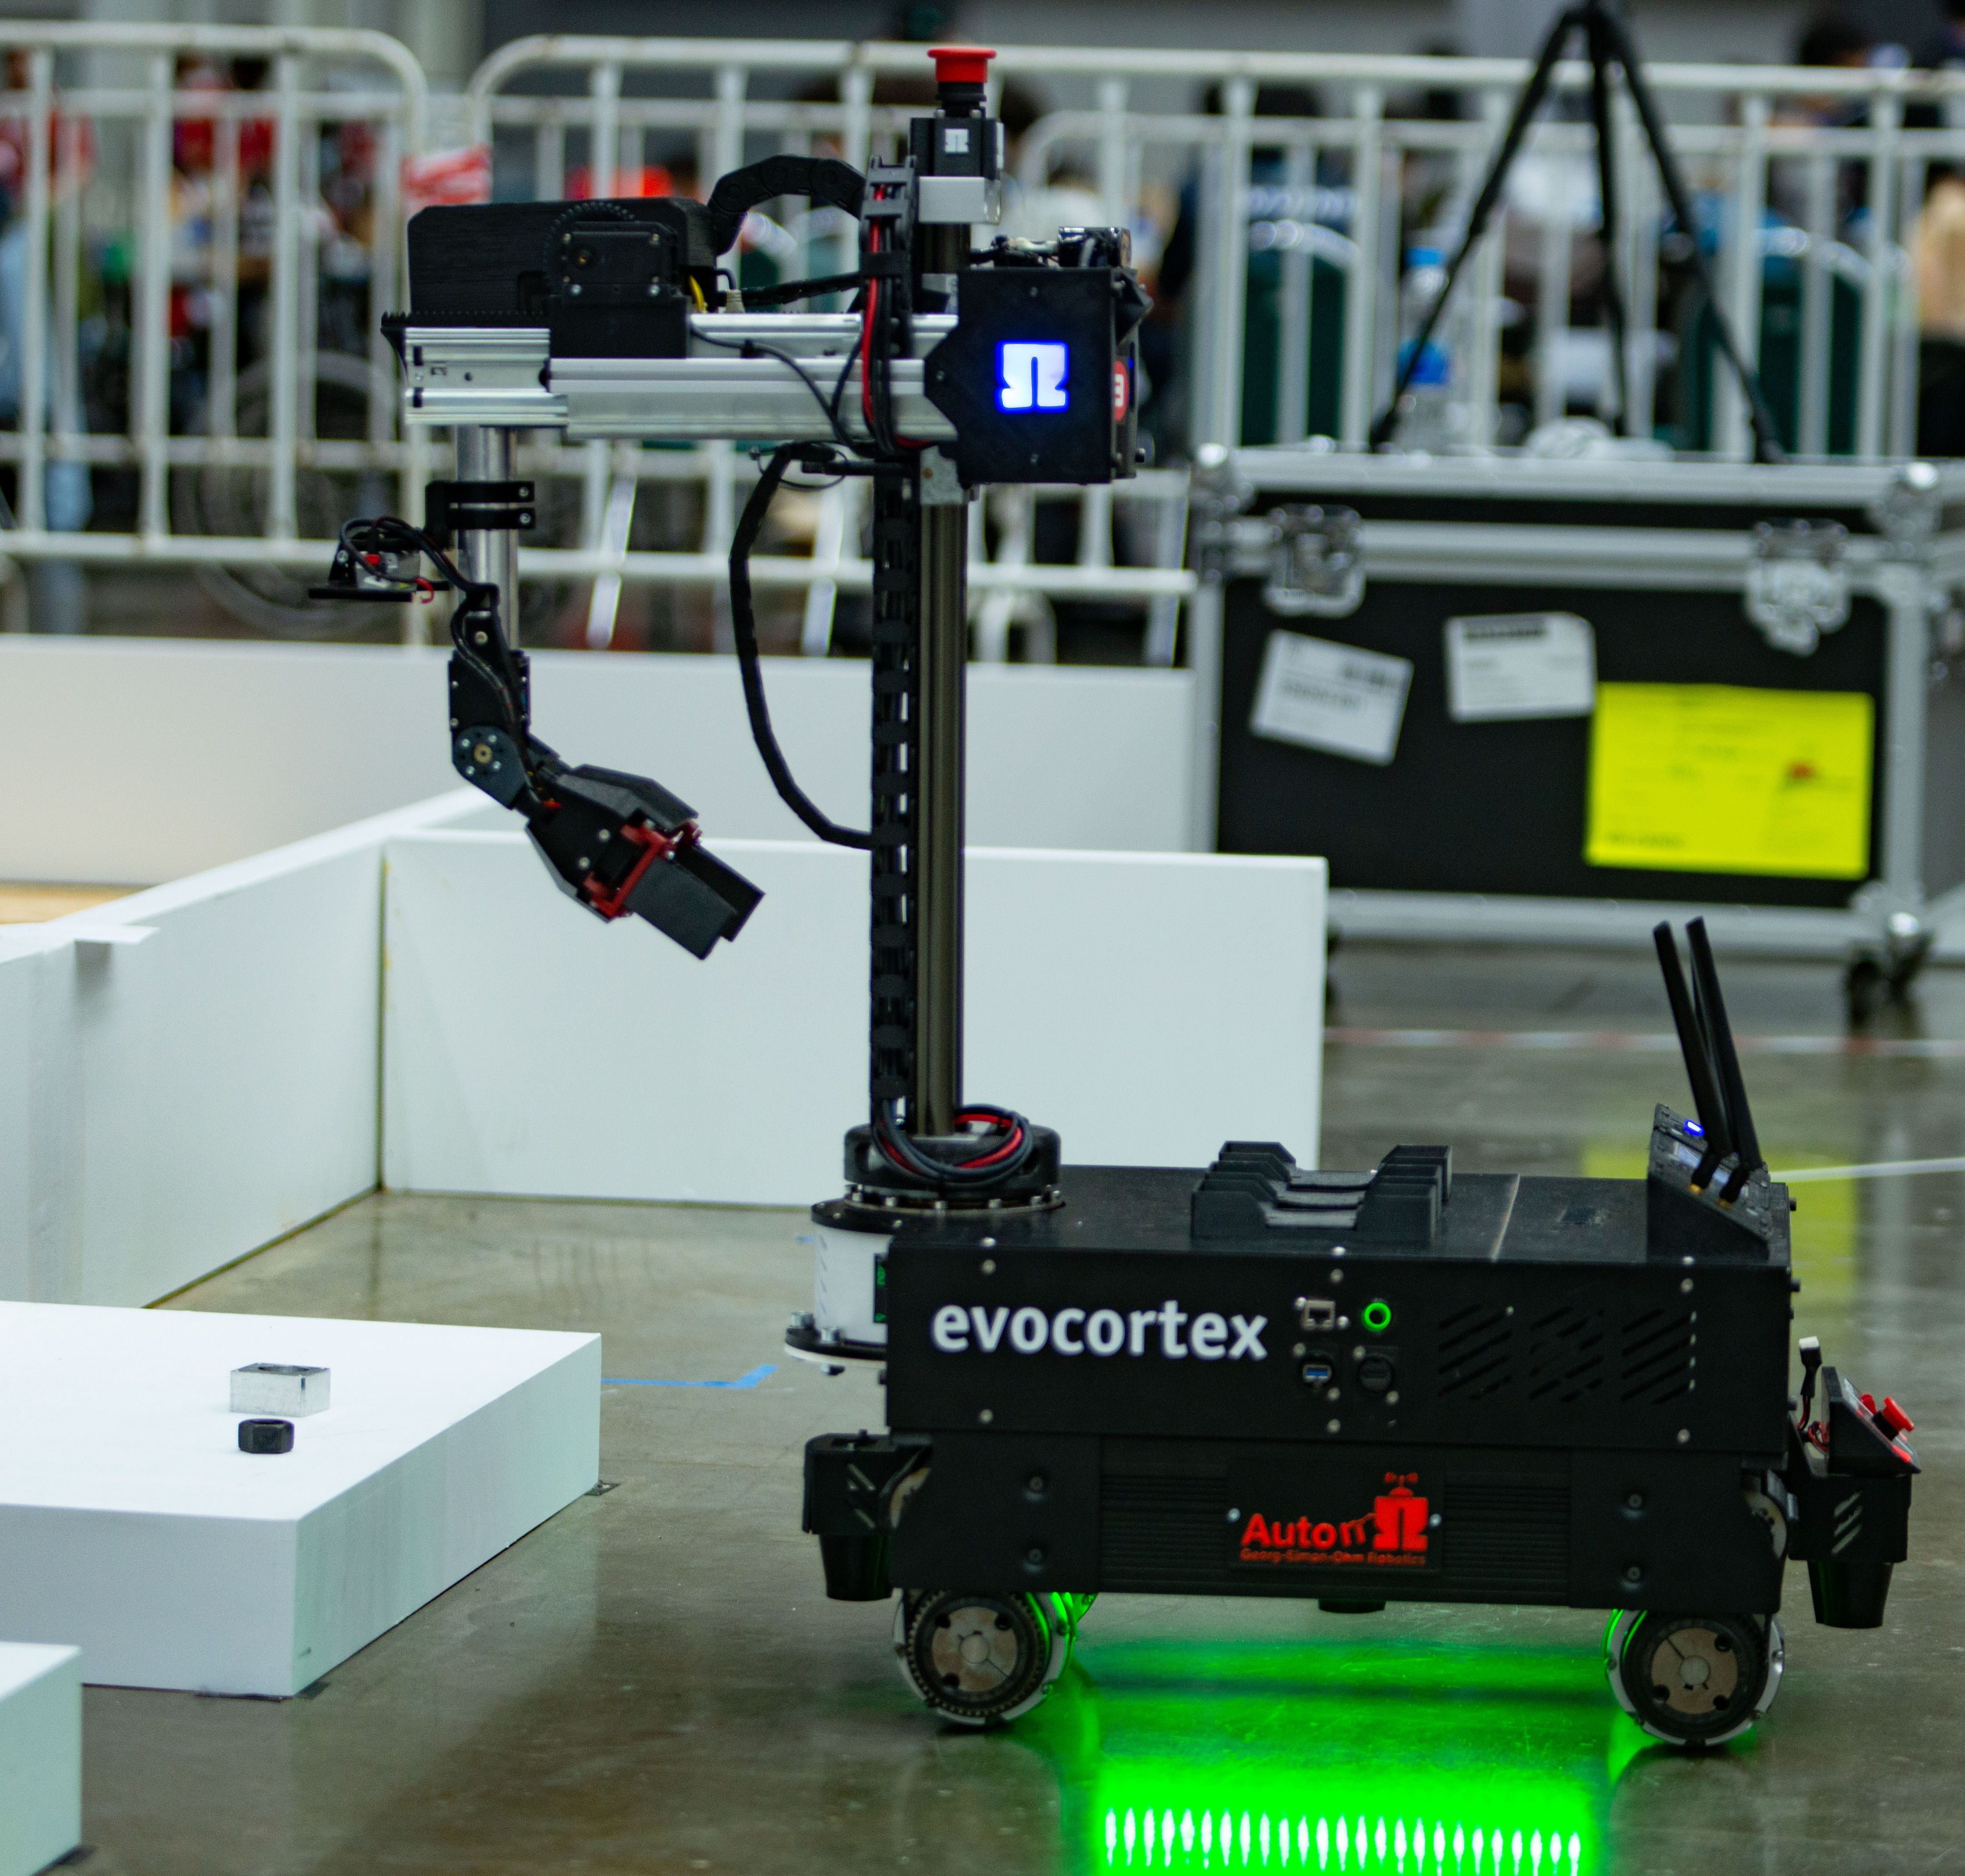
\includegraphics[width=0.3\textwidth]{./images/robots/AutonOhm_Ohmn3.jpg}} \hfill
		\subfloat{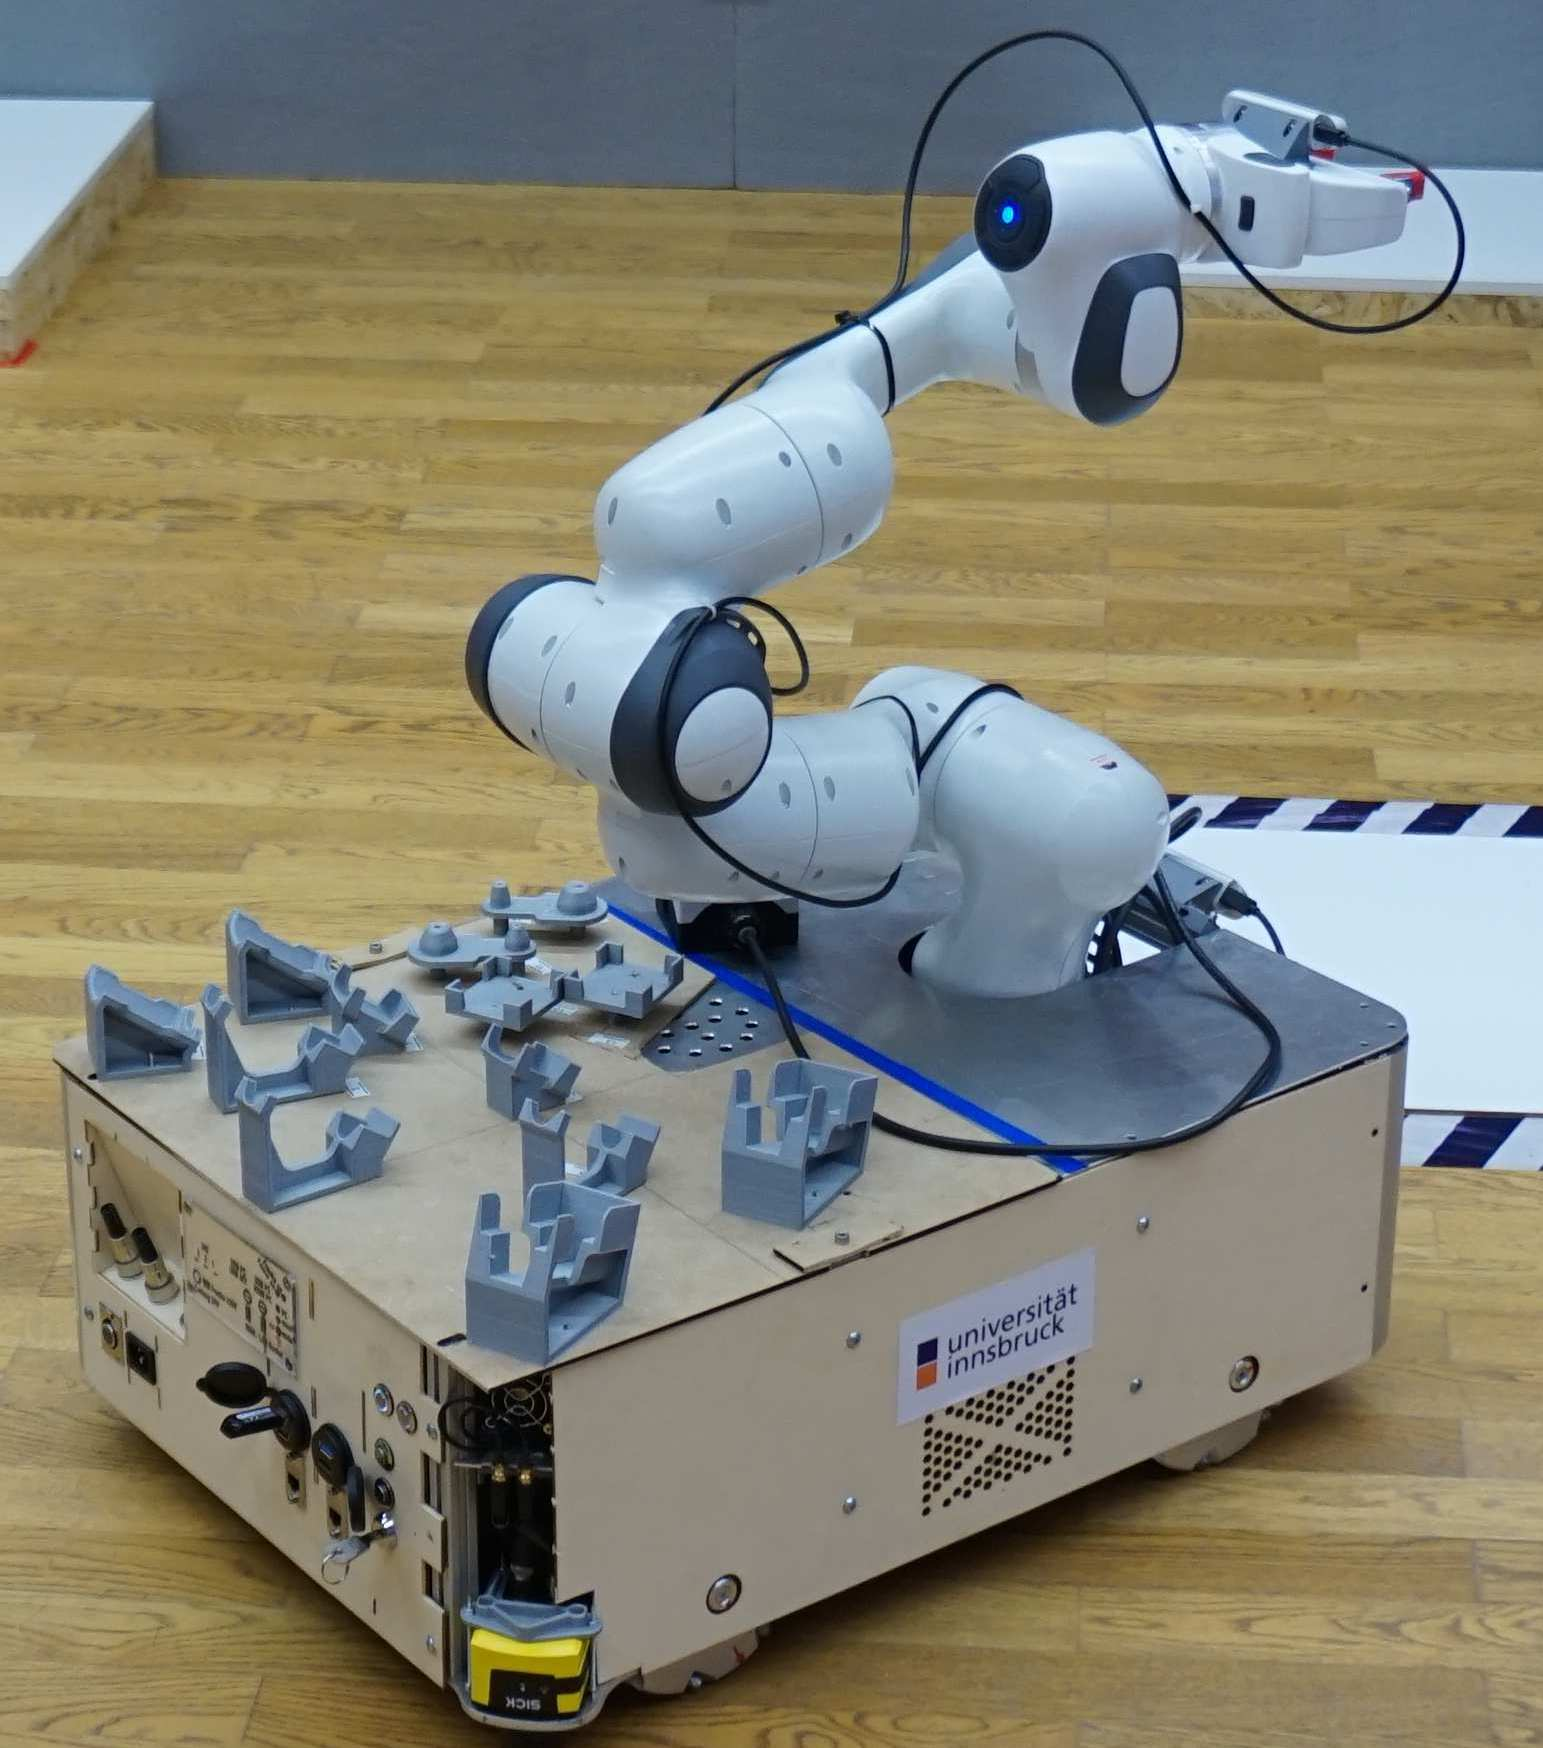
\includegraphics[width=0.31\textwidth]{./images/robots/tyrolics2.jpg}} \hfill
		\subfloat{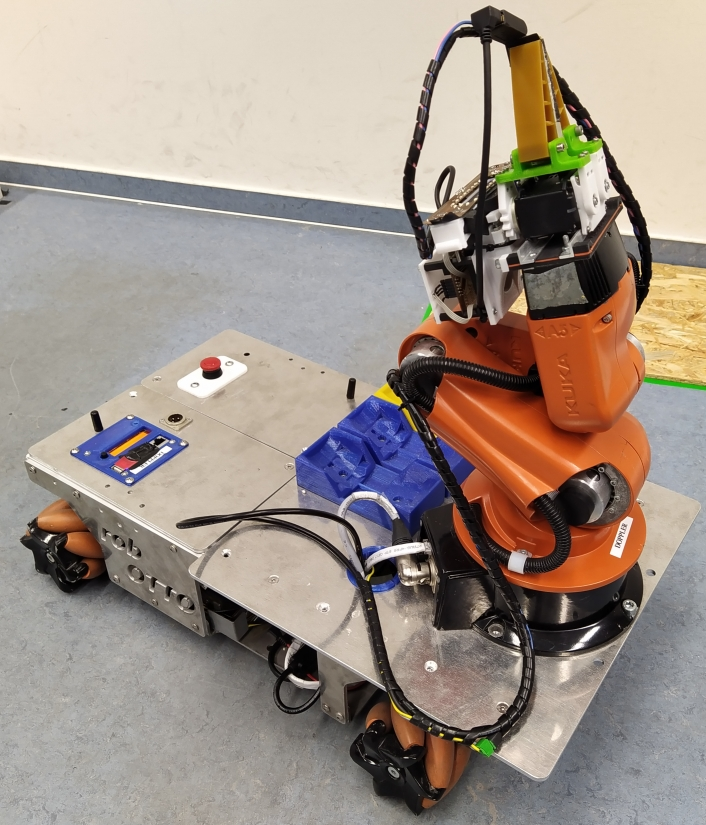
\includegraphics[width=0.3\textwidth]{./images/robots/robotto_bot_small.jpg}} 
	\end{center}
	\caption{Examples mobile robot platforms that can be used for \RCAW. Robots from the teams AutonOHM (Nuremberg-Germany), Tyrolics (Innsbruck-Austria) and robOTTO (Magdeburg-Germany) -- from left to right. }
	\label{fig:example_robots}
\end{figure}


\subsection{Behavior and Safety} \label{ssec:RobotBehaviorAndSafety}
For safety the robots have to meet the constraints in section \ref{ssec:RobotDesignAndConstraints}. In general, all robots shall be operated with maximum safety in mind. Any robot operation must be such that a robot neither harms humans nor damages the environment. 
The used batteries shall be handled with care and all team members must be educated in the correct usage, charging and storage of the batteries of the team. For lithium batteries appropriate storage bags must be used by the teams. The OC supplies a fire extinguisher for lithium batteries at the competition. If this is not sufficient for the used batteries of a team. The team is responsible for supplying an appropriate fire extinguisher by themselfs. The OC and TC control the observance of this rules.

All robots must have an emergency stop button. The emergency stop has to be a hard stop mechanism, that ensures that the energy transfer to all actuators is stopped immediately and the robot halts. The mechanism must be a red emergency stop button that is clearly visible, easily accessible and per wire attached to the robot. It has to be easy accessible from at least 3 sides of the robot. A wireless emergency stop button is optional but not sufficient.

The OC may request the proof of a robot's safety (e.g. the correct operation of an emergency stop) anytime during the competition and exclude teams that cannot satisfy safety requirements.

When participating in a competition, the team may operate the robot only in their own team area, in the arenas provided (possibly constrained by a schedule assigning periods of time for exclusive use of the arena by a team or a group of teams), and in any other areas designated by the organizers for robot operation. Any operation of robots outside of these areas, e.g. in public areas or emergency paths, require prior permission by the OC.

\textbf{Safety test procedure:}

Before the competition starts each robot has to perform a safety test procedure. This will be included in the competition schedule given by the OC.
\begin{itemize}
	\item Inspection of the robot platform (sharp edges and general construction)
	\item Description of the included safety systems by the team leader 
	\item Test of emergency stop while standing still
	\item Test of emergency stop during navigation 
	\item Test of emergency stop during manipulation
\end{itemize}


\clearpage

\section{Arena Environment}
\label{sec:ArenaDesign}
The competition is held in an arena resembling an example layout of industrial manufacturing facilities. In this Section different parts of the environment are explained.

\subsection{Floor}

The floor is made of some firm material. This includes among others floors made of concrete, screed, timber, plywood, chipboard, laminated boards, linoleum, PVC flooring, or carpet. Some examples are illustrated in Figure \ref{fig:example_floors}. Floors may neither be made of loose material of any kind (gravel, sand, or any material which may damage the functioning of the robot's wheels) nor may such material be used on top of the floor. Liquids of any kind are not allowed. The floor may have spots of unevenness of up to $1\si{\centi\meter}$ in any direction (clefts, rifts, ridges, etc.).


\begin{figure} [h!]
	\begin{center}
		\subfloat{
\includegraphics[height = 2cm]{./images/general_rules/example_floor_1.jpg}} \hspace{0.1cm}
		\subfloat{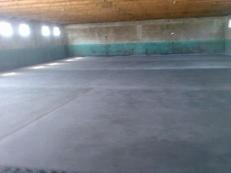
\includegraphics[height = 2cm]{./images/general_rules/example_floor_2.jpg}} \hspace{0.1cm}
		\subfloat{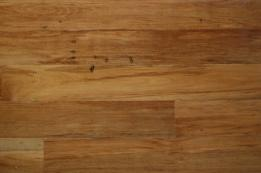
\includegraphics[height = 2cm]{./images/general_rules/example_floor_3.jpg}} \hspace{0.1cm}
		\subfloat{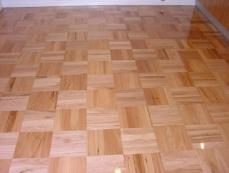
\includegraphics[height = 2cm]{./images/general_rules/example_floor_4.jpg}} \hspace{0.1cm}
		\subfloat{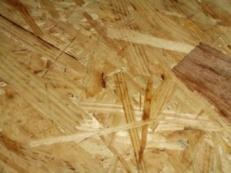
\includegraphics[height = 2cm]{./images/general_rules/example_floor_5.jpg}}\\
		\subfloat{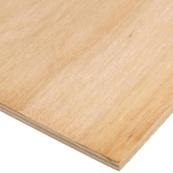
\includegraphics[height = 2cm]{./images/general_rules/example_floor_6.jpg}} \hspace{0.1cm}
		\subfloat{
\includegraphics[height = 2cm]{./images/general_rules/example_floor_7.jpg}} \hspace{0.1cm}
		\subfloat{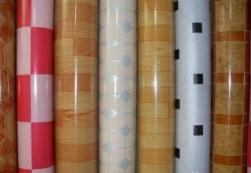
\includegraphics[height = 2cm]{./images/general_rules/example_floor_8.jpg}} \hspace{0.1cm}
		\subfloat{
\includegraphics[height = 2cm]{./images/general_rules/example_floor_9.jpg}} \hspace{0.1cm}
		\subfloat{
\includegraphics[height = 2cm]{./images/general_rules/example_floor_10.jpg}}
	\end{center}
	\caption{Examples of floors that can be used for \RCAW arenas.}
	\label{fig:example_floors}
\end{figure}



\subsection{Walls and Virtual Walls}
\label{subsec: Walls and virtual Walls}

The arena consists of outer and inner Walls used to build structures, create obstacles or function as protection barriers for teams and viewers. Walls may be either physical (plank) or virtual (red/white Tape). All walls (physical and virtual) have an infinitely height.
The arena is completely enclosed by Walls (both types possible), meaning robots are not allowed to exit the arena during a run. All types of Walls won't be changed during the competition. If the robot touches a Wall or Virtual Wall it results in a Major Collision.

The height of a physical Wall must be not less than $20\si{\centi\meter}$ and not more than $40\si{\centi\meter}$ (but will be seen as infinite high). Most Walls have a uniform main color (white), but may be enforced by metal (aluminum framework) and decorated with sponsor logos or ads.

Virtual Walls are made of red/white Tape and may never be crossed during a run. The arena can contain Walls and Virtual Walls inside.

\begin{figure} [h!]
\centering
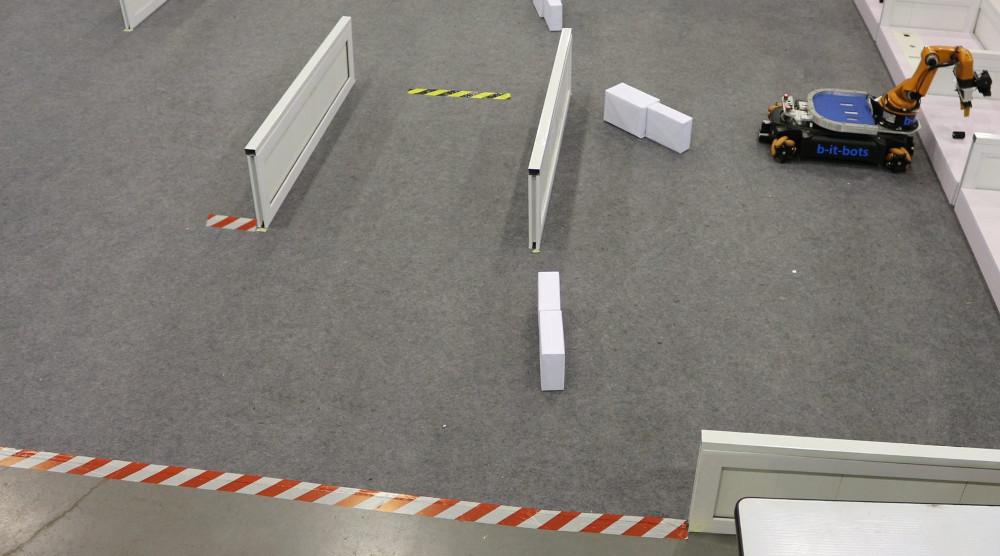
\includegraphics[width= 0.8\textwidth ]{./images/general_rules/barrier_tapes_in_china15.jpg}
\caption{Example of a typical arena. The red/white Tape indicates a Virtual Wall. The yellow/black Tape indicates a Virtual Obstacle and the white ashlar-formed cartonages are Obstacles.}
\label{fig:walls_and_virt_walls}
\end{figure}

\subsection{Obstacles}
\label{subsec: Obstacles}

In addition to the static arena elements, semi-dynamic Obstacles may be placed inside the arena before a competition run begins. 
The position of such Obstacles is decided by the TC during the setup phase of the run and randomized between different run types. Obstacles can be either physical or virtual.

Obstacles may block paths partly or completely, as long as all active Service Areas are still reachable.
There are three main Obstacle placement types:

\begin{itemize}
\item \textbf{Blocking:} 
A narrow section is completely blocked by the Obstacle, which means that no robot can physically pass it ($<$ $20\si{\centi\meter}$).

\item \textbf{Semi-Blocking:} 
The Obstacle reduces the distance between arena elements below the minimum width for a path ($<$ $80\si{\centi\meter}$). The path therefore counts as blocked, meaning that there must exist another valid path to all active Service Areas. Robots are still allowed to use all paths if they fit through the smaller gaps.
The gap width is fixed and its value is calculated using the width of the biggest robot in the competition plus $ 10\si{\centi\meter}$. This usually adds up to around $ 60\si{\centi\meter}$,
but might be higher or lower, depending on the participating robots.

\item \textbf{Non-Blocking:}
The Obstacle adds or enlarges an arena element but keeps all paths intact.
\end{itemize}


Physical Obstacles (see figure \ref{fig:walls_and_virt_walls}) measure atleast $2\si{\centi\meter}$ x $2\si{\centi\meter}$ x $20\si{\centi\meter}$ (l x w x h) and may be made of any non-transparent, firm material (wood, metal). Some examples are bins, shipping boxes and Wall elements. Their color is not specified.
All physical Obstacles are treated like any other arena element during a run, including the rules for collisions (Major Collision).

Virtual Obstacles are marked using the yellow/black Tape from section \ref{subsec:Tapes}. The collisions with these Virtual Obstacles will treated as Tape Collision (see \ref{sec:penalties}).


\subsection{Tapes}
\label{subsec:Tapes}

\textbf{Red/white Tape:}

The red/white Tape (Tesa signal $5\si{\centi\meter}$ width) is considered as a Virtual Wall and has an infinite height. The red/white Tape is static and won't be changed during the whole competition. It will be used inside the arena and as an outer border of the arena.  Touching the red/white Tape is considered as a Major Collision.

\textbf{Yellow/black Tape:}

The yellow/black Tape (Tesa signal $5\si{\centi\meter}$ width) is considered as a Virtual Obstacles and has an infinite height. The yellow/black Tape will be placed by the TC before a run that contains Virtual Obstacles. Touching the yellow/black Tape is considered as a Tape Collision.

\begin{figure} [h!]
	\centering
	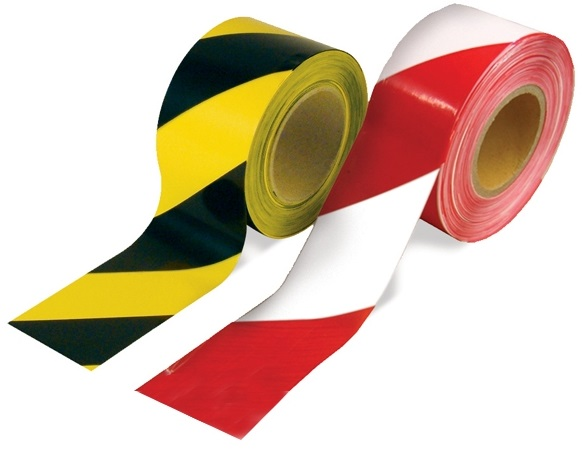
\includegraphics[width= 0.4\textwidth ]{./images/general_rules/example_barrier_tape}
	\caption{Example red/white and yellow/black Tapes}
	\label{fig:tapes}
\end{figure}

\textbf{Markup Tape:}

Green electrical tape is considered as markup Tape. This tape can be used everywhere, where it is useful. It is intended as a marker for the referees and teams and not for the robot. Therefore the color may deviate, but the color is not red or yellow to guarantee a clear difference to the other tapes. The tape is used to mark the START and FINISH area. Furthermore the tape can be used to mark the position of tables (especially $0\si{\centi\meter}$) and Walls. The latter ones are useful for restoring the arena in case of a Major Collision.


\subsection{Tables}
\label{subsec: Tables}

%52. However, from 2020 on and in order to make the competition more realistic, the heights of the Tables will be variable, allowing the OC to adjust them before each test run.-> No???
%-> every height of the Tables can have a margin of $2\si{\centi\meter}$
%-> Table height “fixed”, but may change due to Arbitrary Surface (margin of $2\si{\centi\meter}$)
%Leander

%54. Define Table Size:
%-> 80cm x 50cm x X cm (0, 5, 10, 15)
%-> same size for shelf
%Leander

%However, from 2020 on and in order to make the competition more realistic, the heights of the service Areas will be variable, allowing the OC to adjust them before each test run. TODO...



Tables in the league typically measure $80\si{\centi\meter}$ wide (the side the robot approaches) and $50\si{\centi\meter}$ deep. These are the intended dimensions, but a margin of +/- $10\si{\centi\meter}$ is allowed to accommodate potential construction variations. In general terms, the table shall be big enough to contain at least one manipulation zone as described in section \ref{ssec:ManipulationZone}. In general two manipulation zones are included on one table (one zone on each side of the Table). The used table heights are $0\si{\centi\meter}$, $5\si{\centi\meter}$, $10\si{\centi\meter}$ and $15\si{\centi\meter}$. See further down in this section for more information about the $0\si{\centi\meter}$-Table. See figure \ref{fig:ws} for illustration. 
The tolerance for the heigth is $\pm 2 \si{\centi\meter}$. During a competition the Table size is only fixed in the margin of $\pm 2 \si{\centi\meter}$, because of arbitrary surfaces (see \ref{subsec:Arbitrary_Surfaces_and_Decoys} for an explanation of arbitrary surfaces). 
The table is closed between the bottom and the table top. That's why the Table can be used as a reference for navigation, when the height is sufficient for the robot. Note that the height may change slightly with arbitrary surfaces during a competition and thus the table can sometimes be visible to the laser scanners and sometimes not. 
 
\begin{figure} [h!]
	\begin{center}
		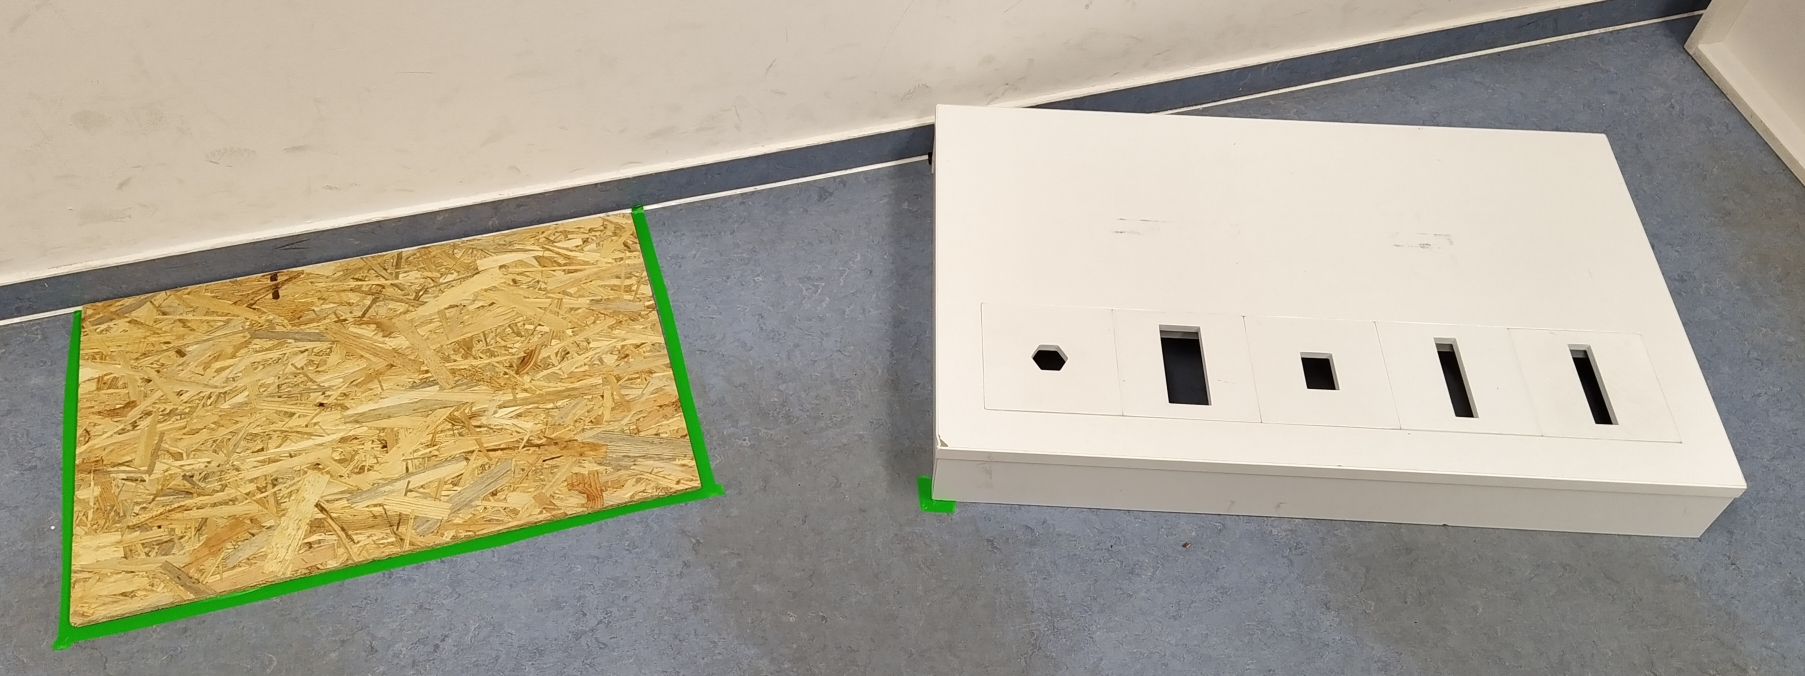
\includegraphics[height = 4cm]{./images/arena/tables_small.jpg}	
	\end{center}
	\caption{left: 0\si{\centi\meter}-Table with arbitrary surface (approx. 1\si{\centi\meter} thick); right: PPT-Table which is a standard 10\si{\centi\meter}-Table with cavities}
	\label{fig:ws}
\end{figure}

If a table has a height of $0\si{\centi\meter}$, a green electrical Tape (see \ref{subsec:Tapes}) will mark the area. A $0\si{\centi\meter}$-Table can be active or inactive. Active means, that the current test (see table \ref{fig:test_specifications_instance}) includes $0\si{\centi\meter}$-Tables.
If the table is active, the surrounded area may be covered by a white sheet of paper or arbitrary surface. The material is not fixed.
The OC is responsible to replace it in case of pollution or tears. To reduce the tear, it is removed when the $0\si{\centi\meter}$-Table is not active. If the floor is white or the table shall have an Arbitrary Surface, no cover needs to be installed.
$0\si{\centi\meter}$-Table may be crossed and does not count as a collision. If the laid out white Surface is moved, it is not a collision.
If the robot touches an Object while navigating, this will be handled as a Minor Collision. Examples for $0\si{\centi\meter}$-Table are shown in figure \ref{fig:0cmws}.



\begin{figure} [h!]
		\begin{center}
			\subfloat{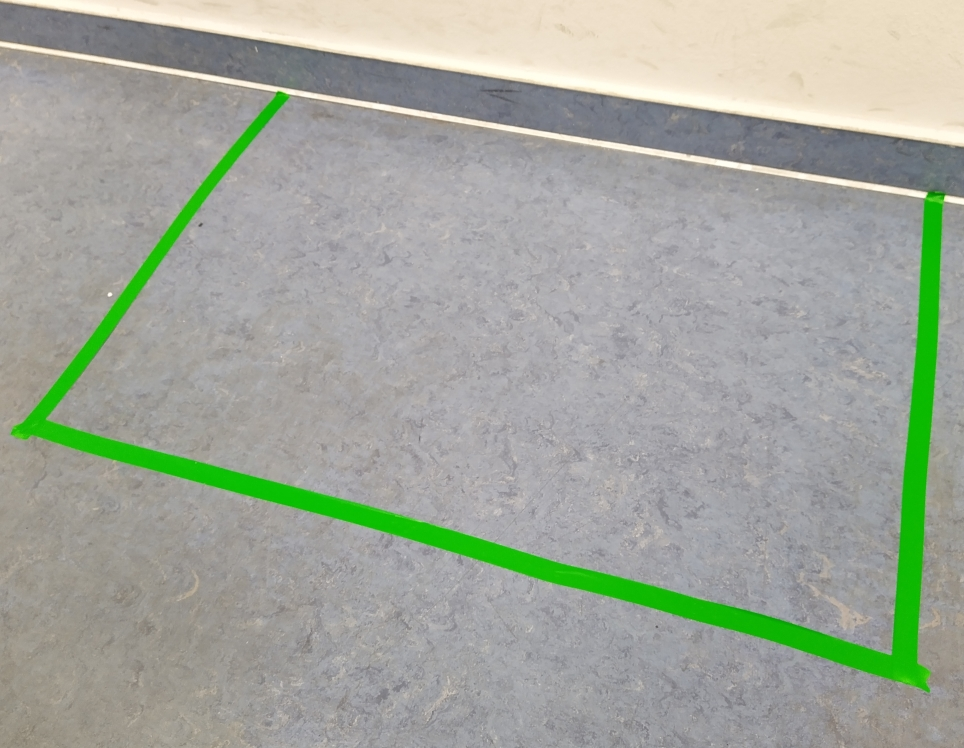
\includegraphics[width=0.4\textwidth]{./images/arena/table_0_inactive_small.jpg}} \hspace{0.2cm}
			\subfloat{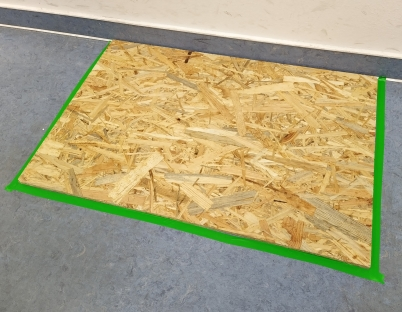
\includegraphics[width=0.4\textwidth]{./images/arena/table_0_arb_small.jpg}} 
		\end{center}
	\caption{left: $0\si{\centi\meter}$-Table which is considered as inactive or as an active table with arbitrary surface; right: $0\si{\centi\meter}$-Table which is considered as active with an arbitrary surface}
	\label{fig:0cmws}
\end{figure}

\subsection{Shelves}\label{sec:Shelves}

The integration of Shelves into tests is according the table \ref{fig:test_specifications_instance}. Service Areas may foresee the use of shelves and shelf units as depicted in Figure~\ref{fig:shelf}. The lower part of the Shelf is a $10\si{\centi\meter}$-Table as specified in \ref{subsec: Tables}.
The maximum height of the shelves should be not more than $40\si{\centi\meter}$. In the example shown in Figure~\ref{fig:shelf} the first $15 \si{\centi\meter}\pm 2\si{\centi\meter} $ are not covered by the top shelf. The length of free space can be changed during competition and can not be seen as mandatory. Therefore all teams has to consider special picking behavior to avoid collision.  

The top shelf surface may be specially designed in order to serve specific purposes, e.g.\, holding Objects. Objects for grasping are always placed on the bottom shelf. The placement of a delivered Object has to be done on the top shelf.  

\begin{figure}[h!]
	\centering
	\subfloat[A shelf with two levels and uniform colored surfaces.]{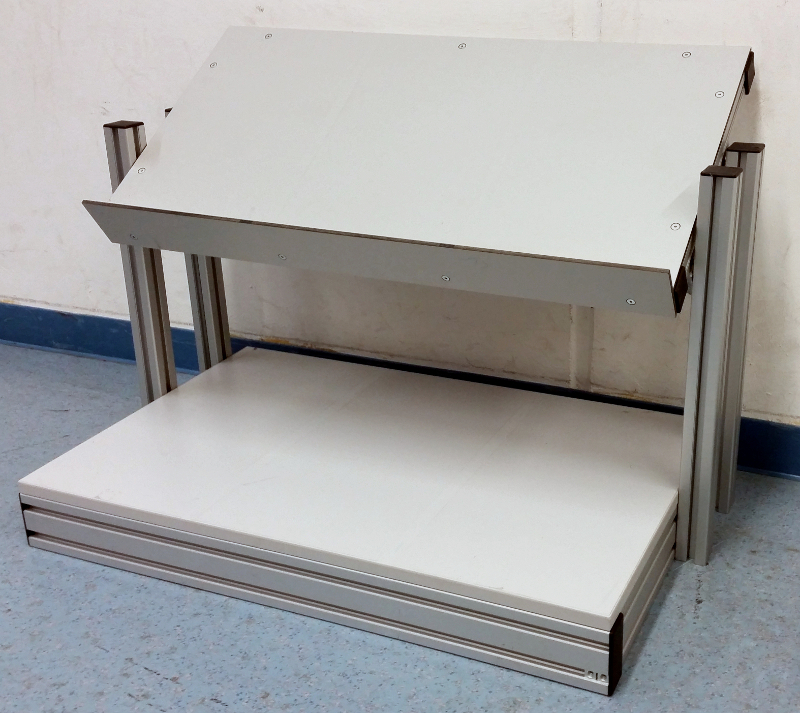
\includegraphics[width=0.375\textwidth ]{./images/shelf.jpg}}
	\hspace{0.05\textwidth}
	\subfloat[Technical draw of shelf configuration.]{ 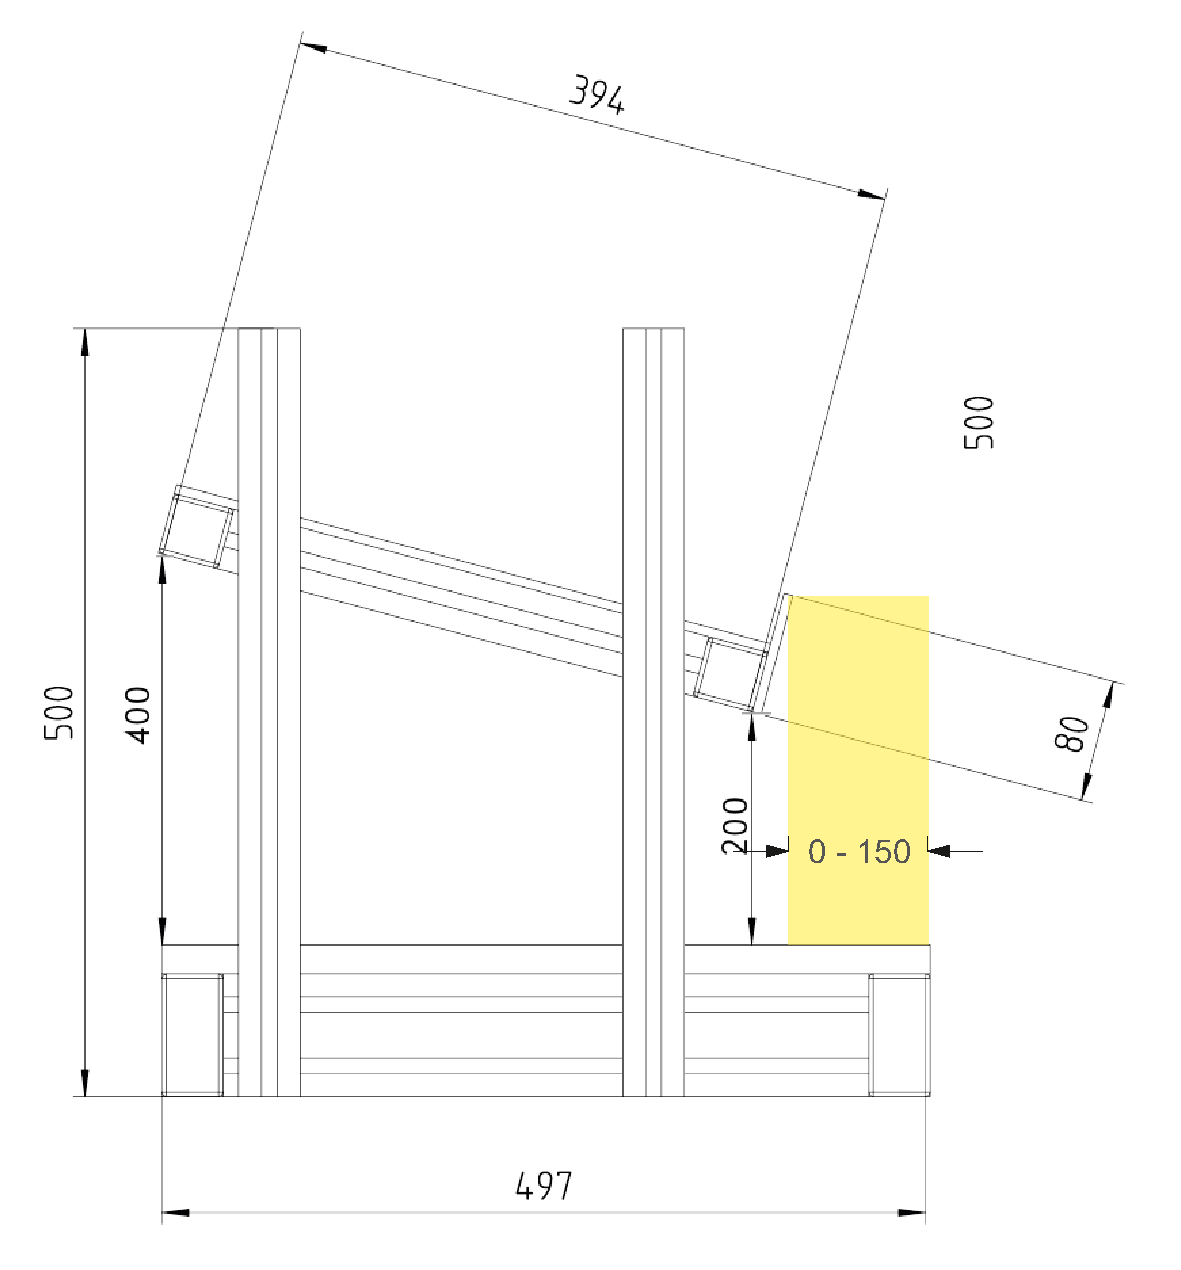
\includegraphics[width=0.375\textwidth ]{./images/shelfUpdate.pdf} }
	\caption{Exemplary shelf and generic technical drawing.}%
	\label{fig:shelf}
\end{figure}


\subsection{Rotating Tables}\label{sec:Rotating Table}
The integration of Rotating Tables into tests is according the table \ref{fig:test_specifications_instance}.  A Rotating Table as depicted in Figure~\ref{fig:rottable} is used for these tests. The Objects placement is the same like in section \ref{ssec:ManipulationZone}, so the maximal depth for Objects is $20 \si{\centi\meter}$ and there is gap of $2\si{\centi\meter}$ to the border of the Rotating Table.


The height of the Rotating Table should be not lesser than $8\si{\centi\meter}$ and not be more than $12\si{\centi\meter}$. The diameter of the Rotating Table should be not lesser than $50\si{\centi\meter}$ and not more than $100\si{\centi\meter}$. The Rotating Table has to have a white surface colour. The rotating speed of the table depends on the diameter so that the Objects speed is able to vary between $5 \si{\centi\meter\per\second} \le v_{object} \le 20 \si{\centi\meter\per\second}$. This has to be adjusted by the referees before a team starts its run to a fixed value (some small variations in boarders of  technical feasibility are allowed). This is changed after each run type to another random chosen value in this range. During the run of a team the speed is static and each team will have the same table speed. Example: For a Rotating Table with diameter $d_{table}=1\si{\meter}$, Objects are placed on a grasp region with the diameter $d_{object}=0.8\si{\meter}$ with $\omega_{table} = \frac{2 \cdot v_{objects} }{d_{grasp}}=\frac{2 \cdot 0.2}{0.8}=0.5\si{\radian\per\second}$ and with $n_{table}=\frac{\omega_{table}}{2 \cdot \pi}=\frac{0.5}{2 \cdot \pi}$ the minimum rotational speed of the Rotating Table $n_{table}= 0.0796 \si{\per\second}$ (rounds per second) can be calculated.  

\begin{figure}[h!]
	\centering
	\subfloat[A Rotationg table with some Objects.]{%
		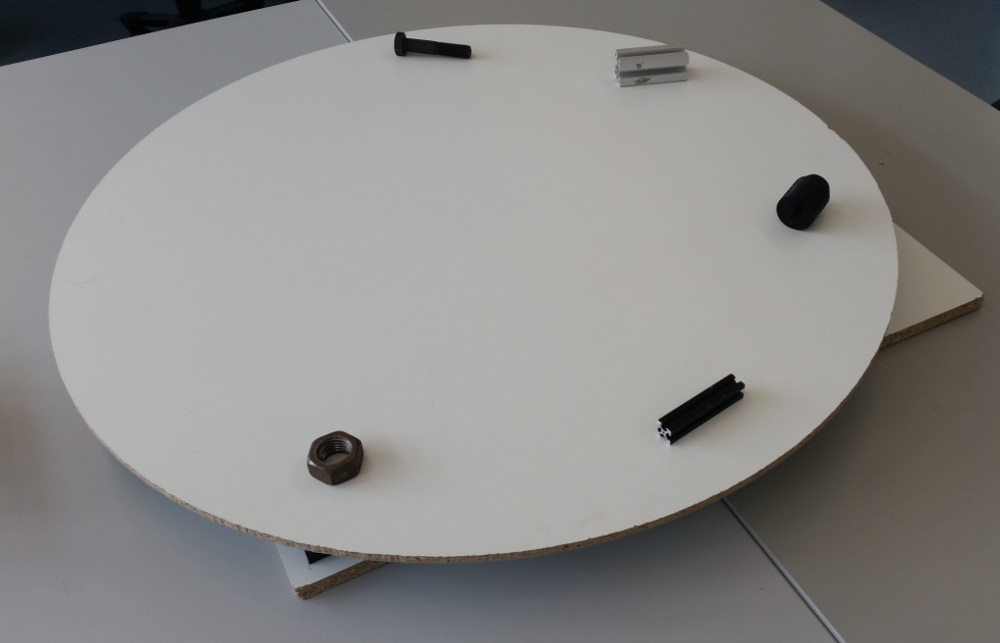
\includegraphics[width=0.375\textwidth,angle=0 ]{./images/rotating_table.jpg}%
	}%
	\hspace{0.05\textwidth}
	\subfloat[Technical draw of Rotating table.]{%
		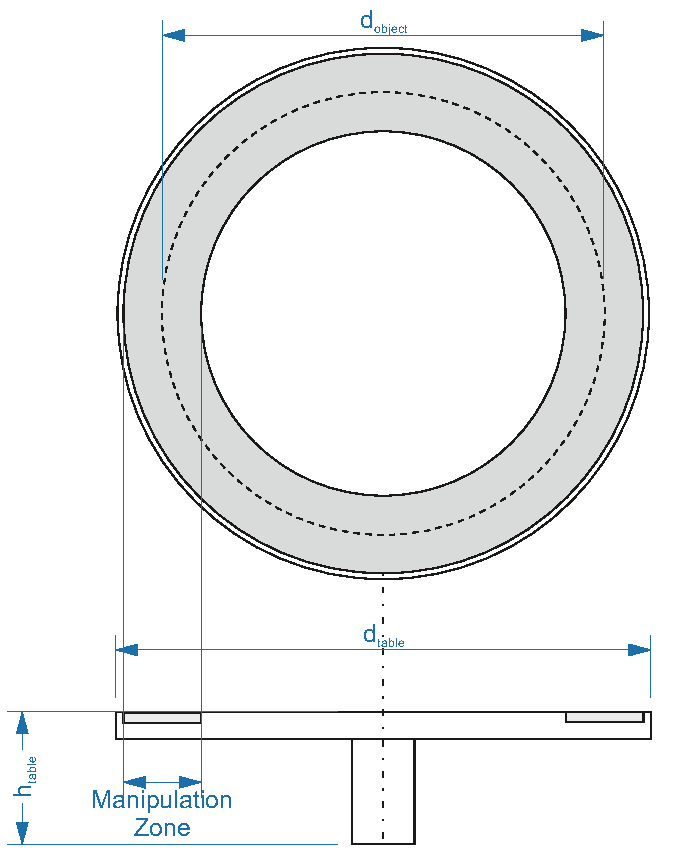
\includegraphics[width=0.375\textwidth ]{./images/rotating_table_schematic.pdf}
	}
	\caption{Exemplary Rotating table and generic technical drawing.}%
	\label{fig:rottable}
\end{figure}


\subsection{Precision Placement Tables}\label{sec:Precision Placement}

The precision placement table as shown in Figure~\ref{fig:ppt_table} includes object-specific cavities tiles as shown in the Figure~\ref{fig:ppt_tiles}. It is based on a standard $10\si{\centi\meter}$ table described in Section~\ref{subsec: Tables}. For each object used in the test, there will be one specific cavity. The cavity has the dimension of the object plus a $2 \si{\milli\meter}$ offset for each dimension. At most five cavities are used in the test. The cavities are in an random order on the table and are located within the standard manipulation zone defined in Figure~\ref{fig:manipulation_zone}. One cavity tile has the dimensions of $140 \si{\milli\meter} \times 140 \si{\milli\meter} $. Placing five cavities on a standard $10\si{\centi\meter}$ table leaves a boarder of $5 \si{\centi\meter}$ on each side of the table. The additional decoy cavity tiles will be chosen by the referees. For the Precision Placement Table only the RoboCup@Work Object Set will be used.
\clearpage

\begin{figure} [h!]
	\begin{center}
		\subfloat[F20\_20]{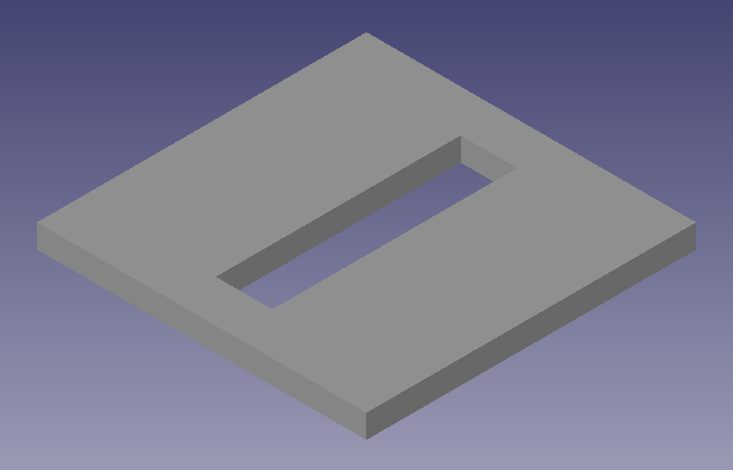
\includegraphics[width = 2cm]{./images/ppt_F20.png}} \hspace{0.1cm}
		\subfloat[S40\_40]{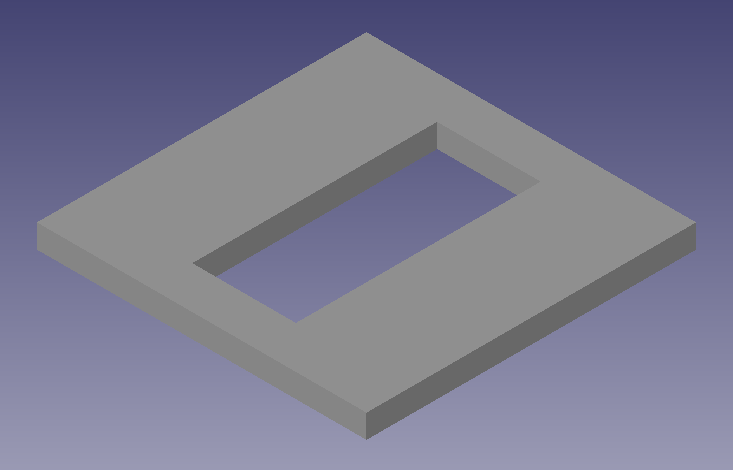
\includegraphics[width = 2cm]{./images/ppt_S40.png}} \hspace{0.1cm} 
		\subfloat[M20\_100]{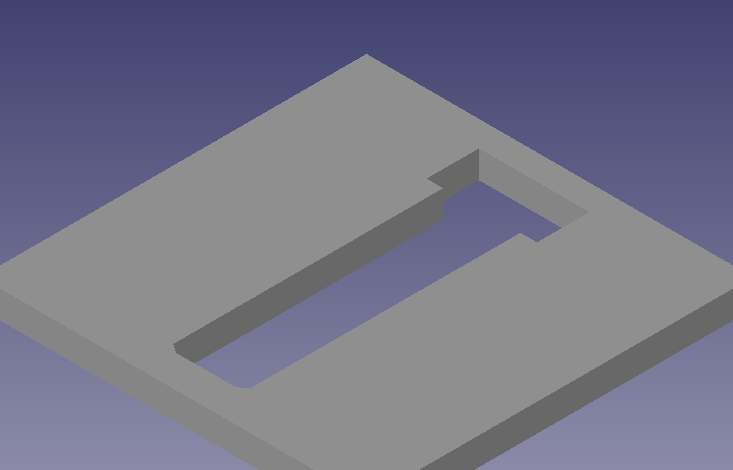
\includegraphics[width = 2cm]{./images/ppt_M20_100.png}}  \hspace{0.1cm}
		\subfloat[M20]{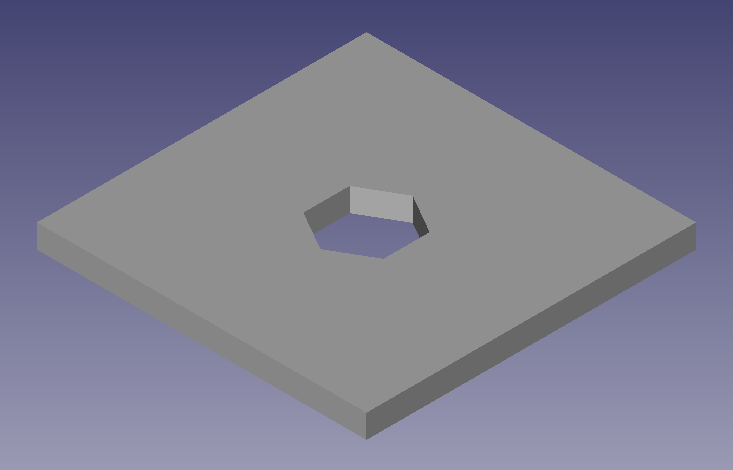
\includegraphics[width = 2cm]{./images/ppt_M20.png}}  \hspace{0.1cm}
		\subfloat[M30]{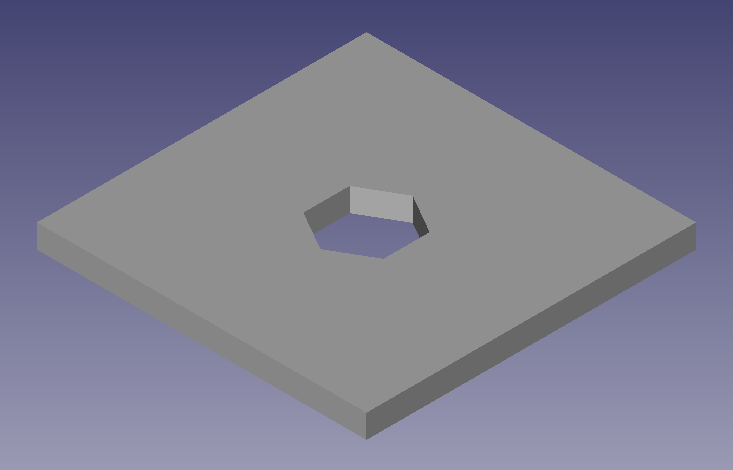
\includegraphics[width = 2cm]{./images/ppt_M30.png}}  \hspace{0.1cm}
		\subfloat[R20]{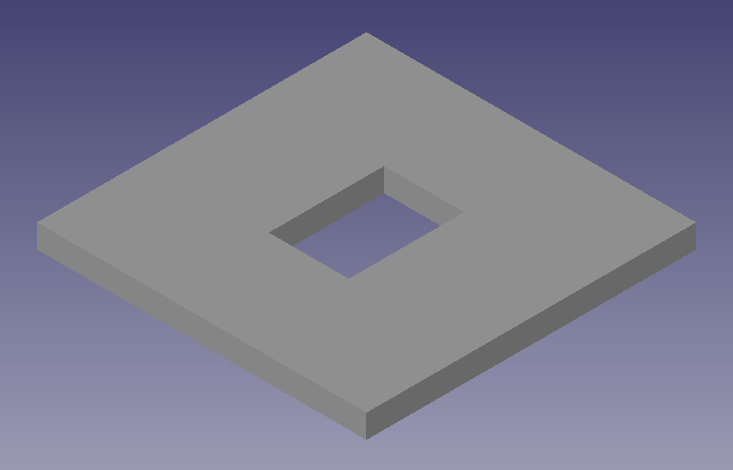
\includegraphics[width = 2cm]{./images/ppt_VR20.png}} \\
		\subfloat[F20\_20]{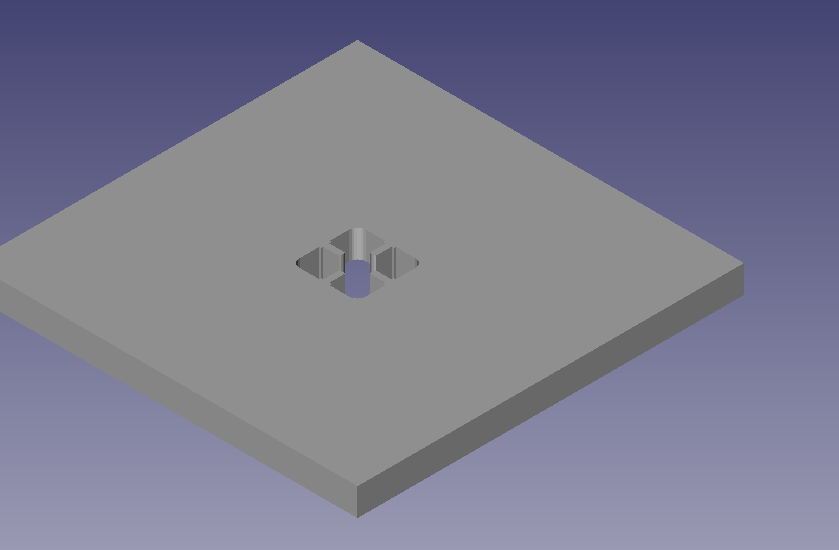
\includegraphics[width = 2cm]{./images/ppt_F20_v.png}}  \hspace{0.1cm}
		\subfloat[S40\_40]{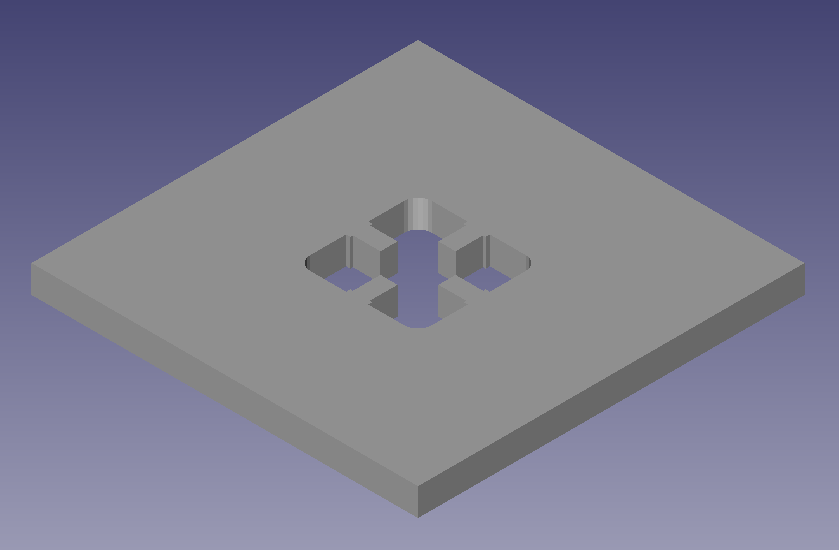
\includegraphics[width = 2cm]{./images/ppt_S40_v.png}}   \hspace{0.1cm}
		\subfloat[M20\_100]{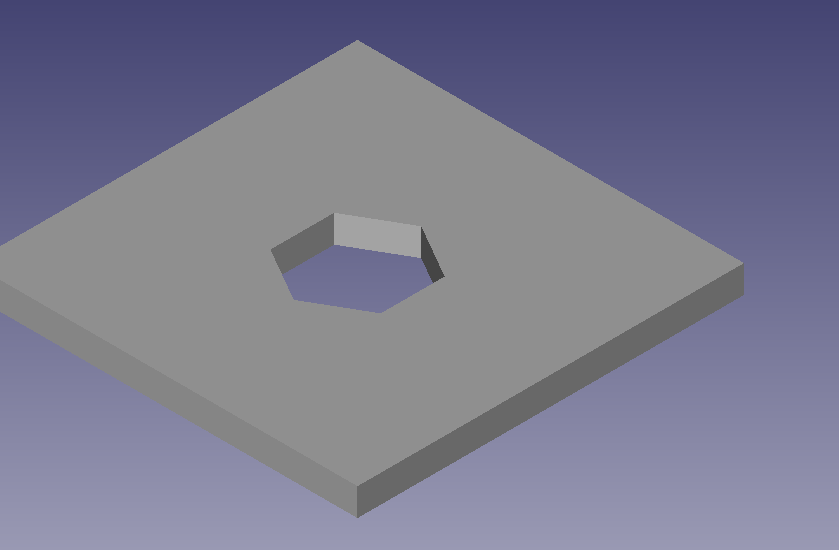
\includegraphics[width = 2cm]{./images/ppt_M20_100_v.png}} \hspace{0.1cm}
		\subfloat[M20]{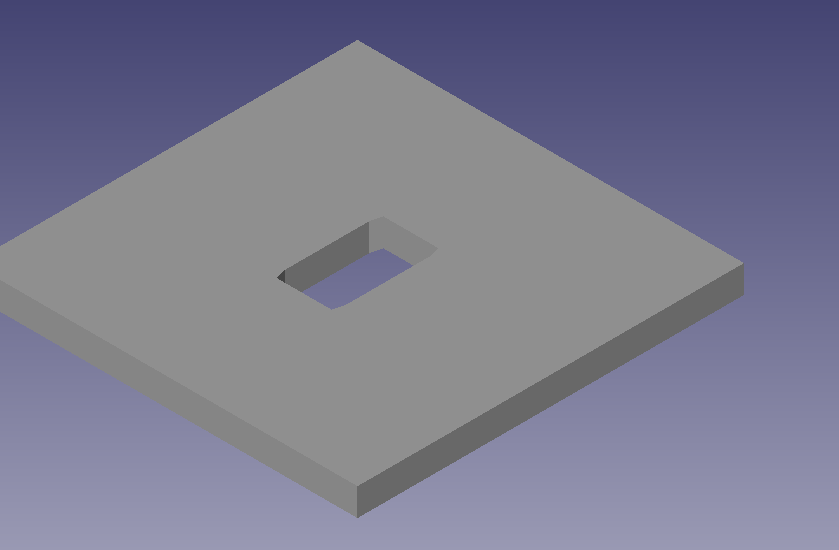
\includegraphics[width = 2cm]{./images/ppt_M20_v.png}}  \hspace{0.1cm}
		\subfloat[M30]{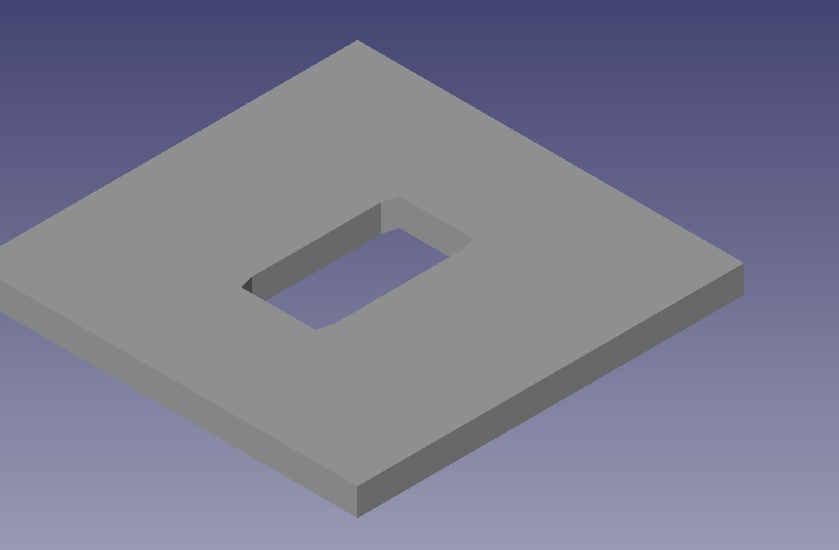
\includegraphics[width = 2cm]{./images/ppt_M30_v.png}}  \hspace{0.1cm}
		\subfloat[R20]{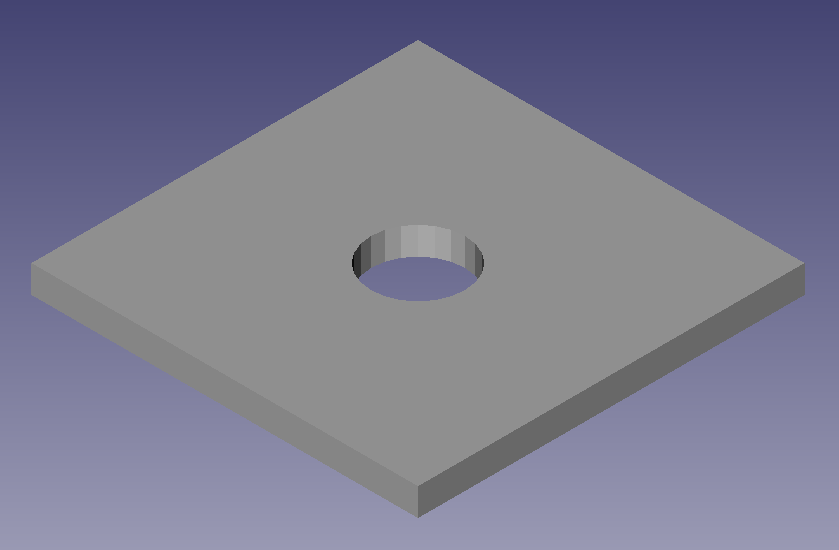
\includegraphics[width = 2cm]{./images/ppt_VR20_v.png}} 
	\end{center}
	\caption{Illustration of horizontal (top row) and vertical (bottom row) cavities for the different kind of manipulation objects.}
	\label{fig:ppt_tiles}
\end{figure}



%\begin{figure} [h!]
%	\centering
%	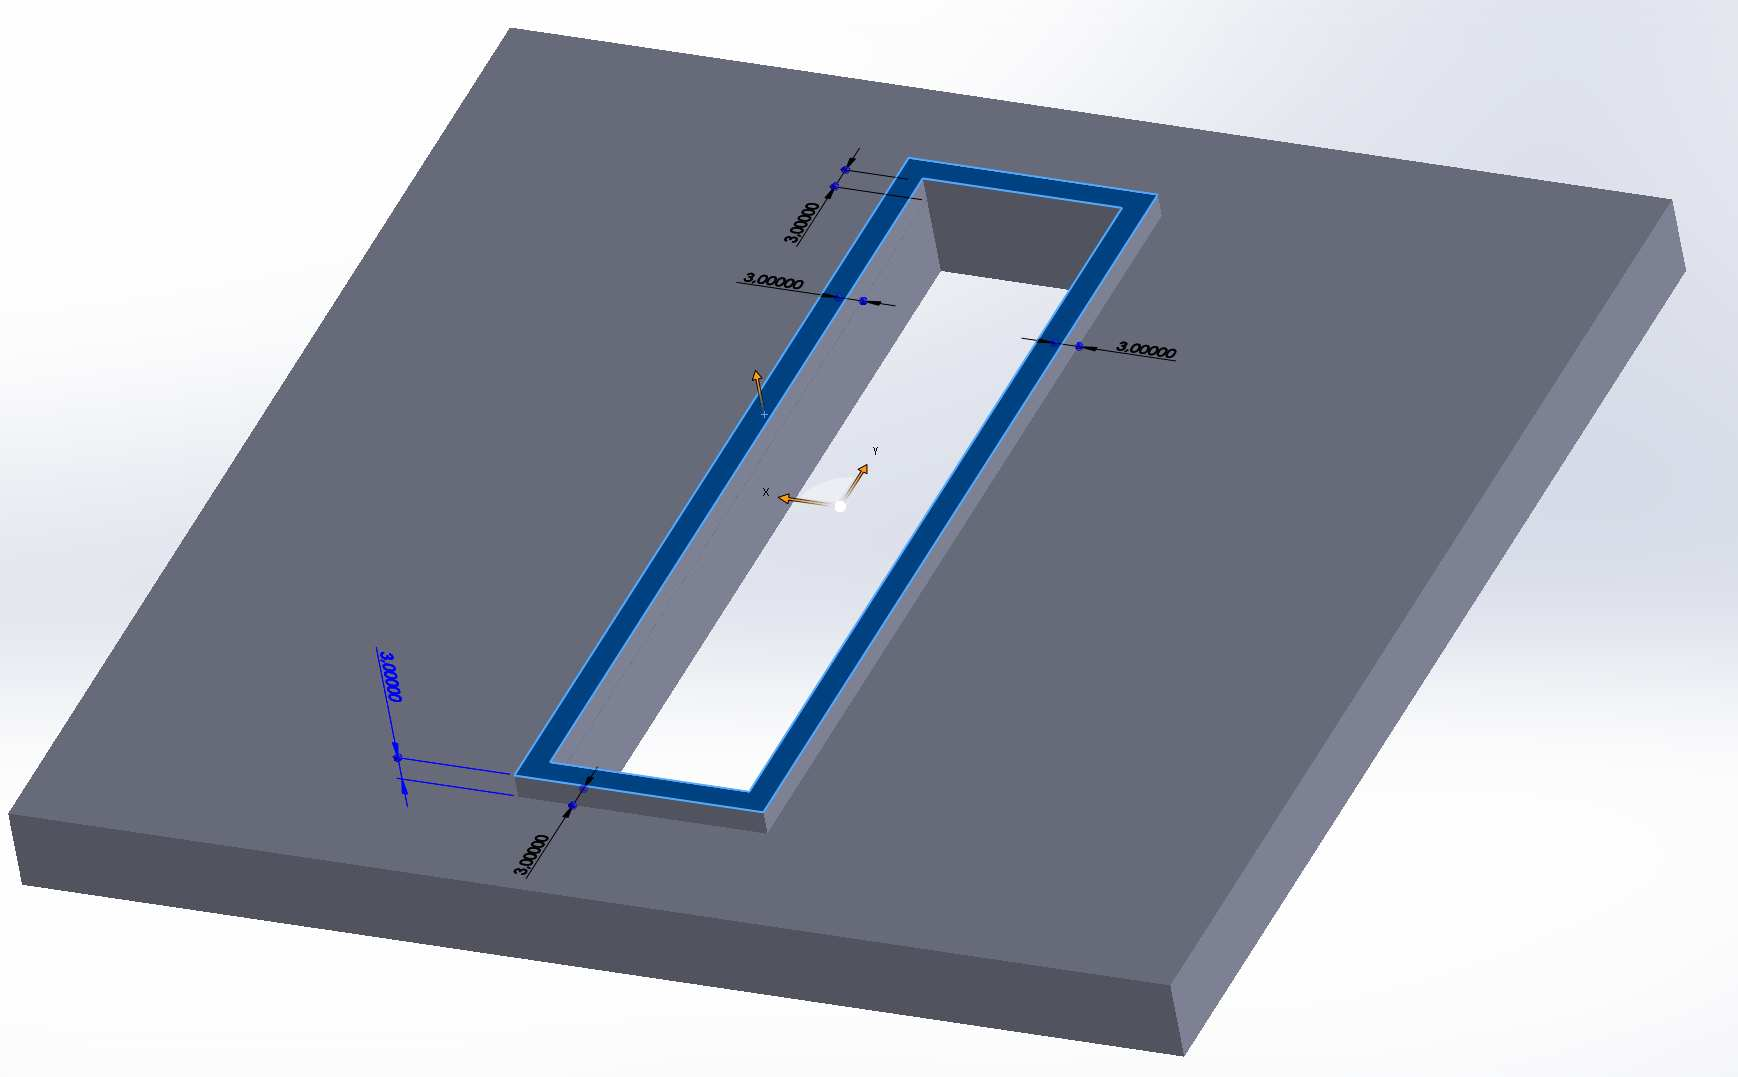
\includegraphics[width= 0.4\textwidth ]{./images/ExampleCavity.jpg}
%	\caption{Example Cavity for F20\_B and G horizontal including $3\si{\milli\meter}$ boarder. }
%	\label{fig:exampleCavity}
%\end{figure}


\begin{figure}[h!]
	\centering

	\subfloat[The PPT platform including five cavity tile.]{%
	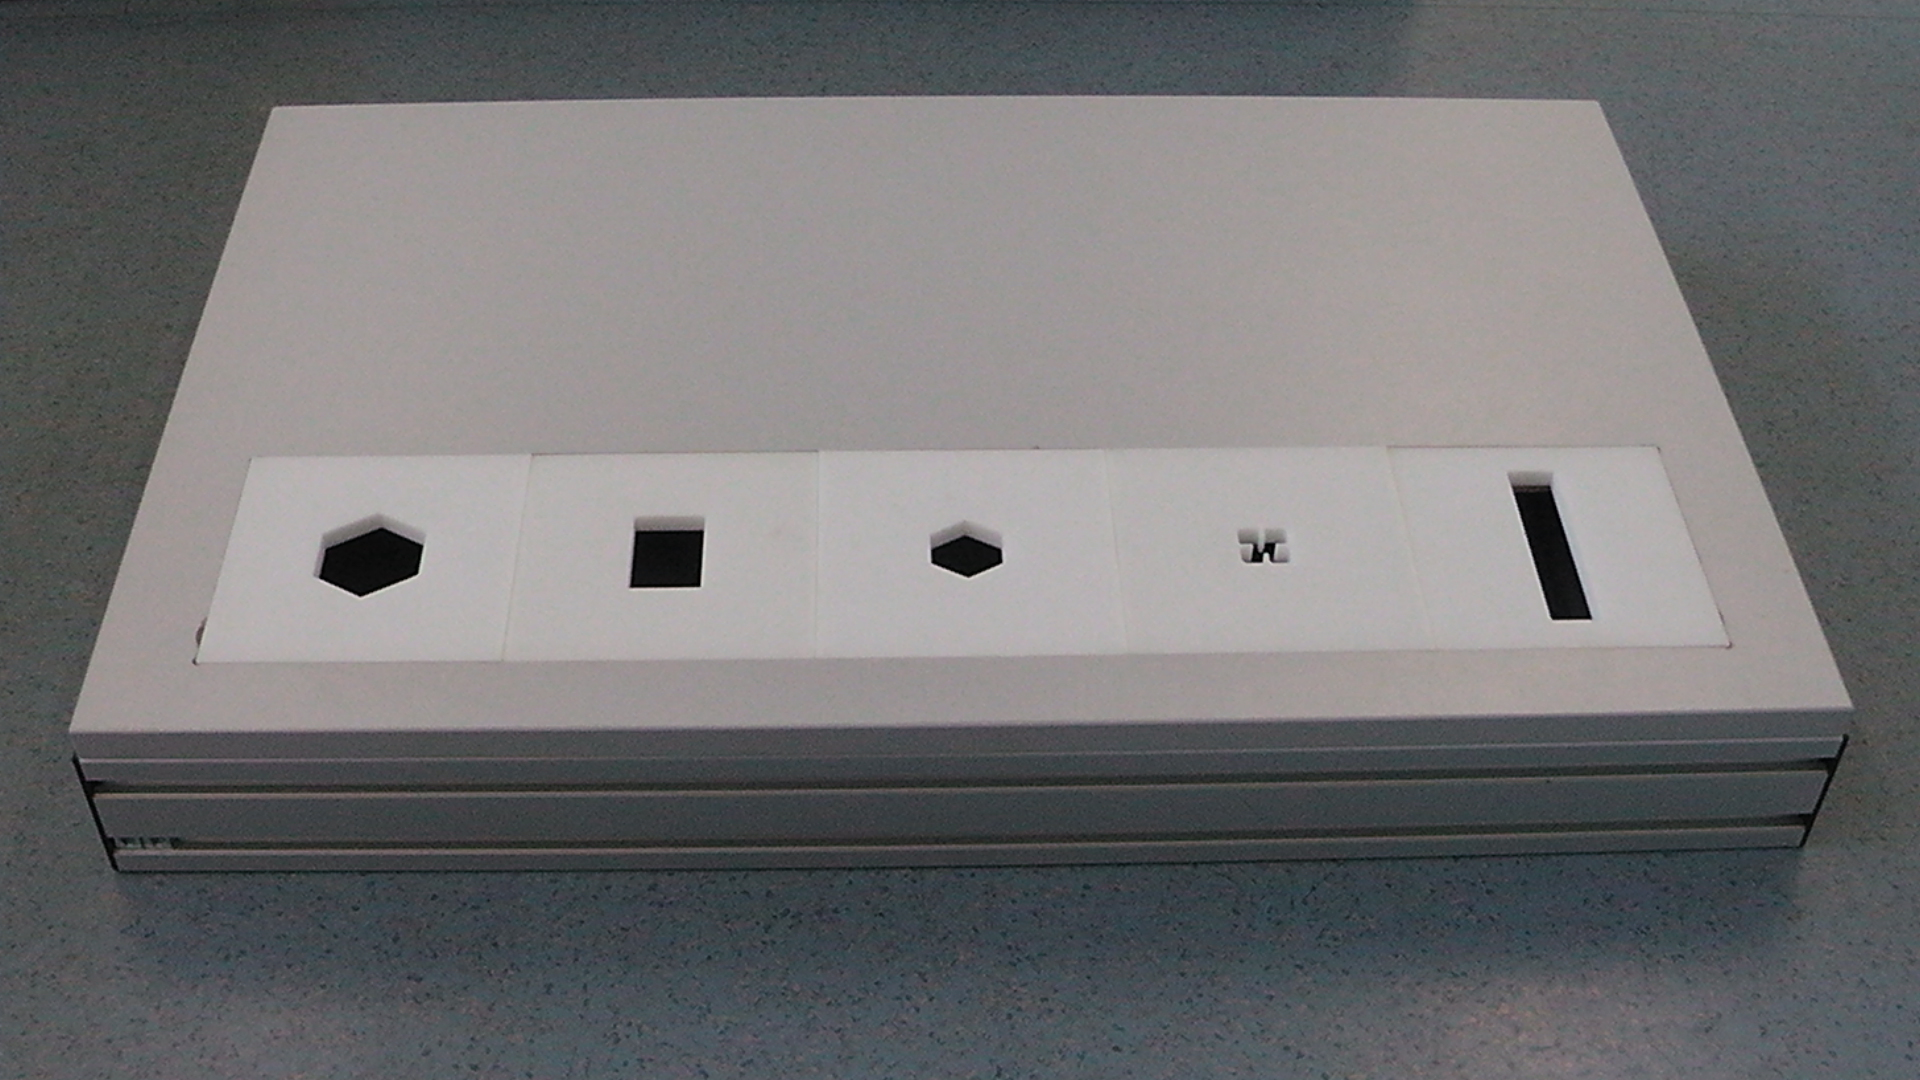
\includegraphics[width=0.45\textwidth ]{./images/ppt_plattform.jpg}
	}%
	\hspace{0.05\textwidth}
	\subfloat[Technical draw of Precision Placement table.]{%
		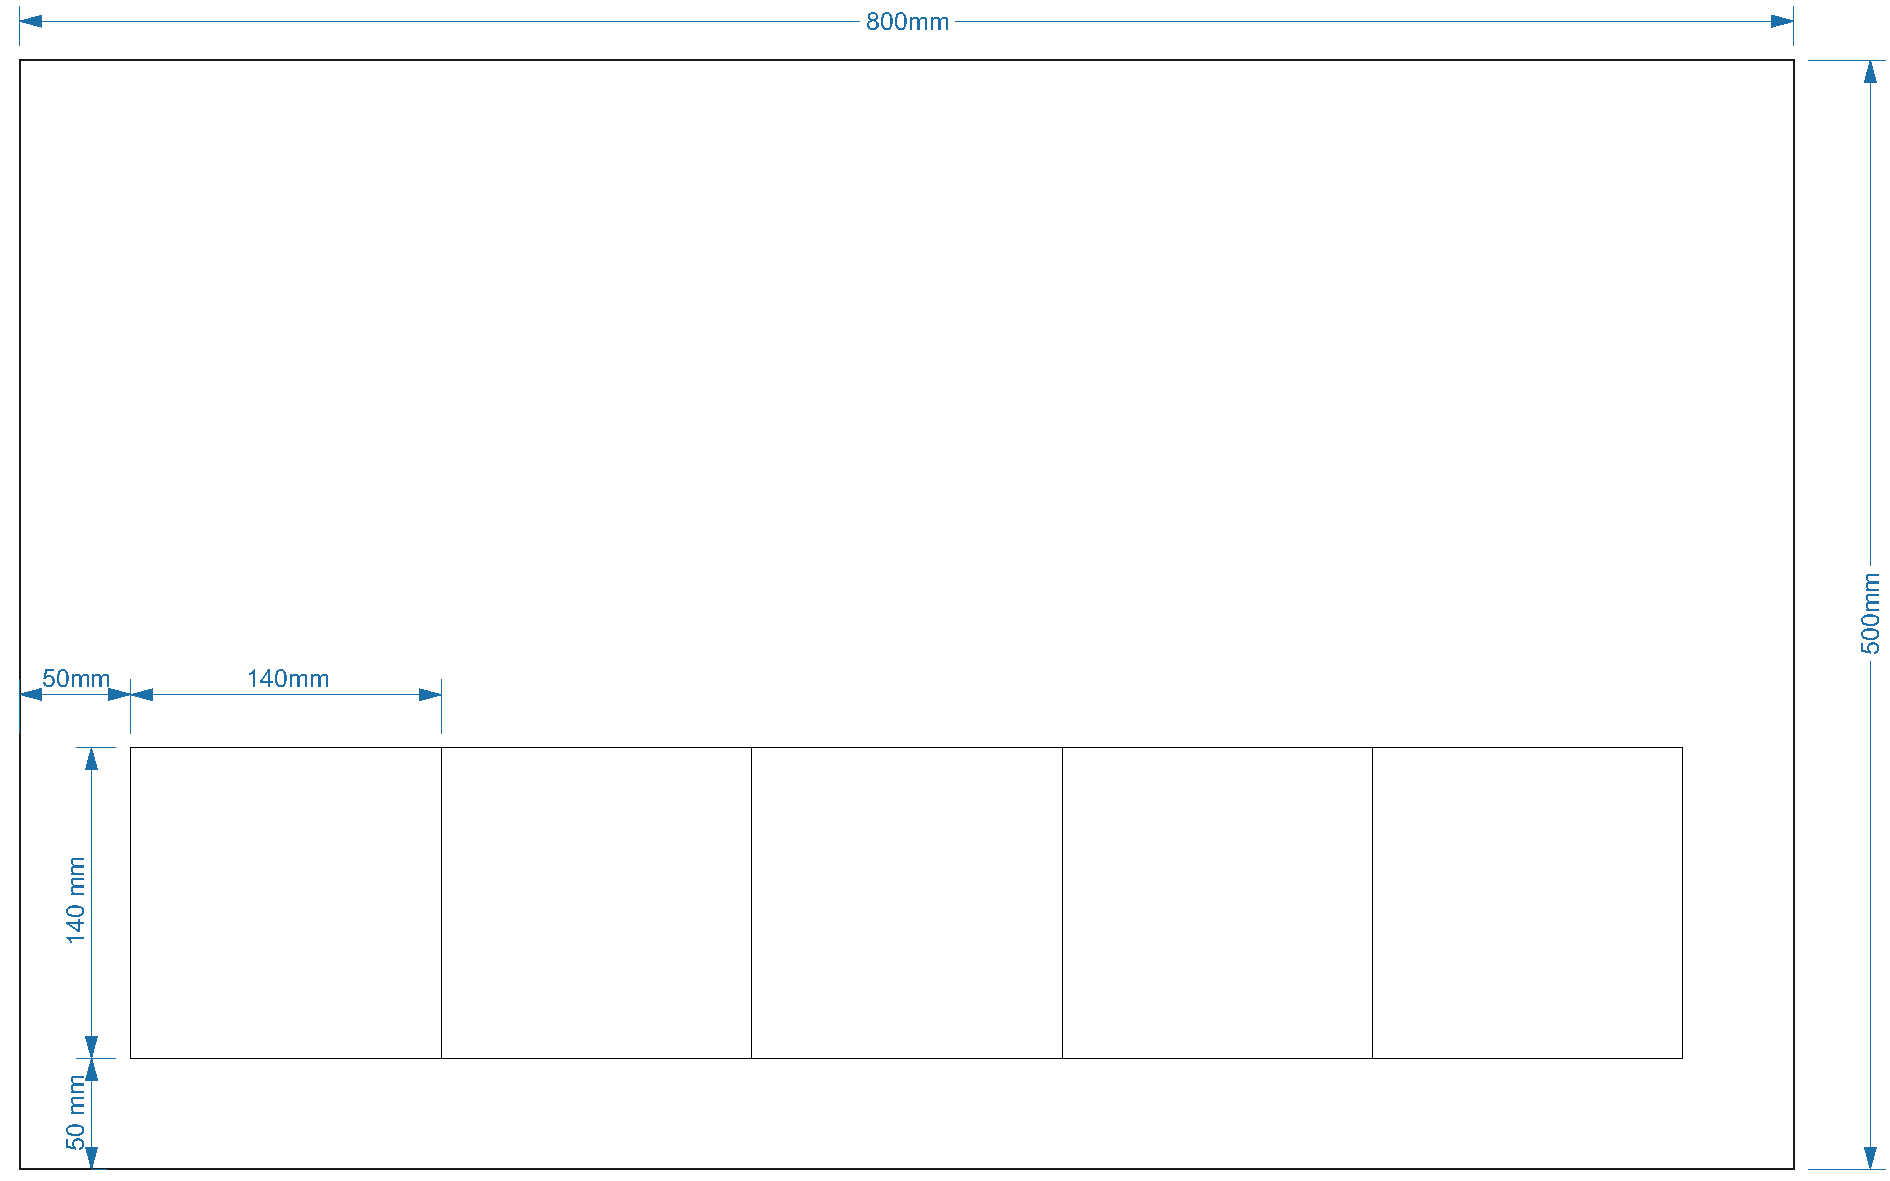
\includegraphics[width=0.45\textwidth ]{./images/PPTtable.pdf}
	}
	\caption{Exemplary Precision Placement table and generic technical drawing.}%
	\label{fig:ppt_table}
\end{figure}



\subsection{Arena Layout}
\label{ssec:ArenaGeneral}

%\textbf{Layout:}
The arena is a static 2D environment consisting of Walls, Tables and Obstacles etc. with a size of atleast 10 m$^2$ and not more than 120 m$^2$. 
An example layout is shown in fig. \ref{fig:arena_example}.

\begin{figure} [h!]
	\centering
	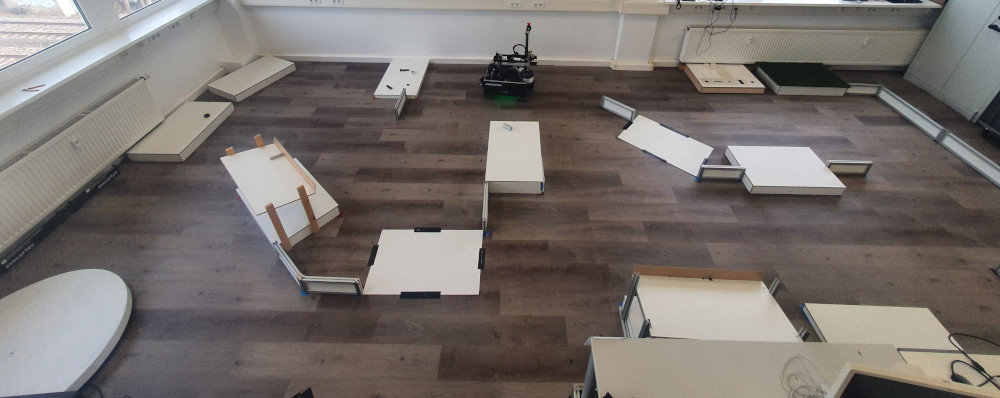
\includegraphics[width= 1\textwidth ]{./images/general_rules/arena_example.jpg}
	\caption{An exemplary setup of a \RCAW environment.}
	\label{fig:arena_example}
\end{figure}

Layouts may include rooms and hallways to create more realistic scenarios.
Service Areas (see section \ref{sec:Service_Areas}) mark the locations for robots to perform tasks.
Each requested Service Area must be accessible via atleast one path of $80\si{\centi\meter}$ width.

\begin{figure} [h!]
	\centering
	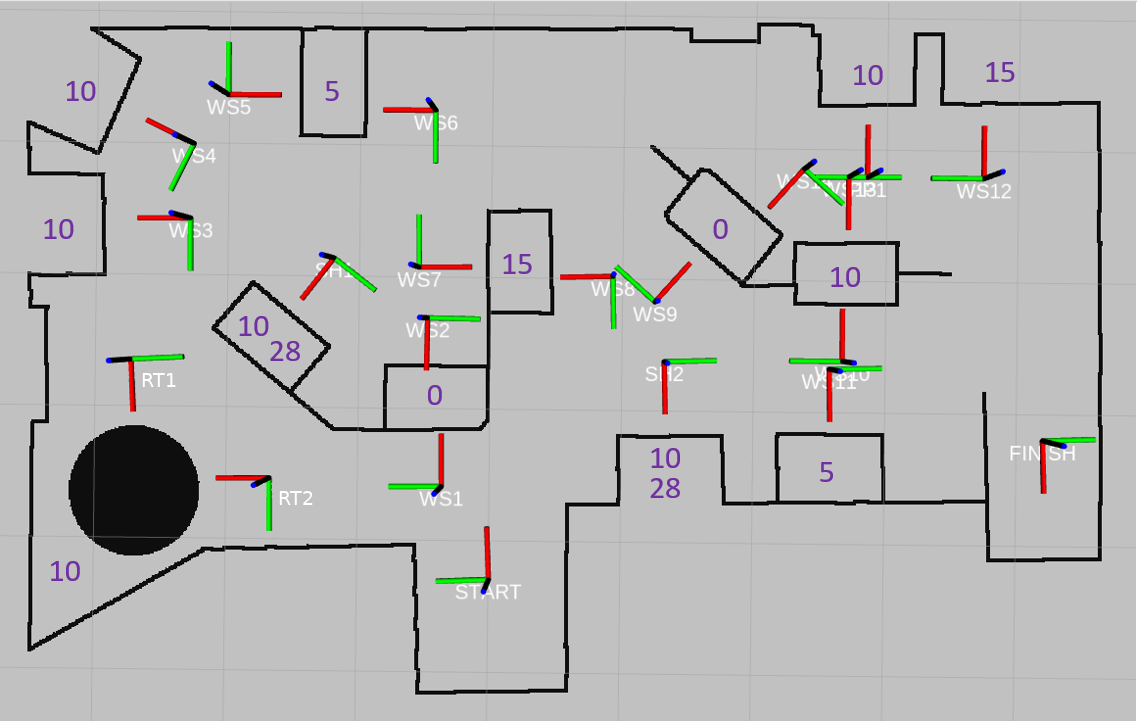
\includegraphics[width= 0.8\textwidth ]{./images/general_rules/arena_map_annotated}
	\caption{Annotated 2D map of the environment in fig. \ref{fig:arena_example}}
	\label{fig:arena_map_annotated}
\end{figure}

Each competition has a new and unique layout designed by the actual TC members.
It should feature:
\begin{itemize}
	\item Area 10 m$^2$ - 120 m$^2$
	\item Minimum distance between arena elements at least $80\si{\centi\meter}$ 
	\item Widespread Service Areas entailing robot movements
	\item Multiple paths between Service Areas
	\item START and FINISH area
\end{itemize}

\clearpage
\textbf{START and FINISH area:}
\label{subsubsec: Start and Goal Area}

One or two parts of the arena are separated with marking Tape and considered as START and FINISH area. The START and FINISH area can be the same or two independent areas. The robot may leave the START area and enter the FINISH area only once. The START/FINISH area is leaved/entered when the robot completely cross the corresponding Marking Tape. In figure \ref{fig:tapeconfig} an exemplary Tape configuration is shown. As soon as the robot enters the FINISH area or re-enters the START area the run ends. The FINISH area counts as a Service Area and reaching the FINISH area gives additional points. 

\begin{figure} [h!]
	\begin{center}
		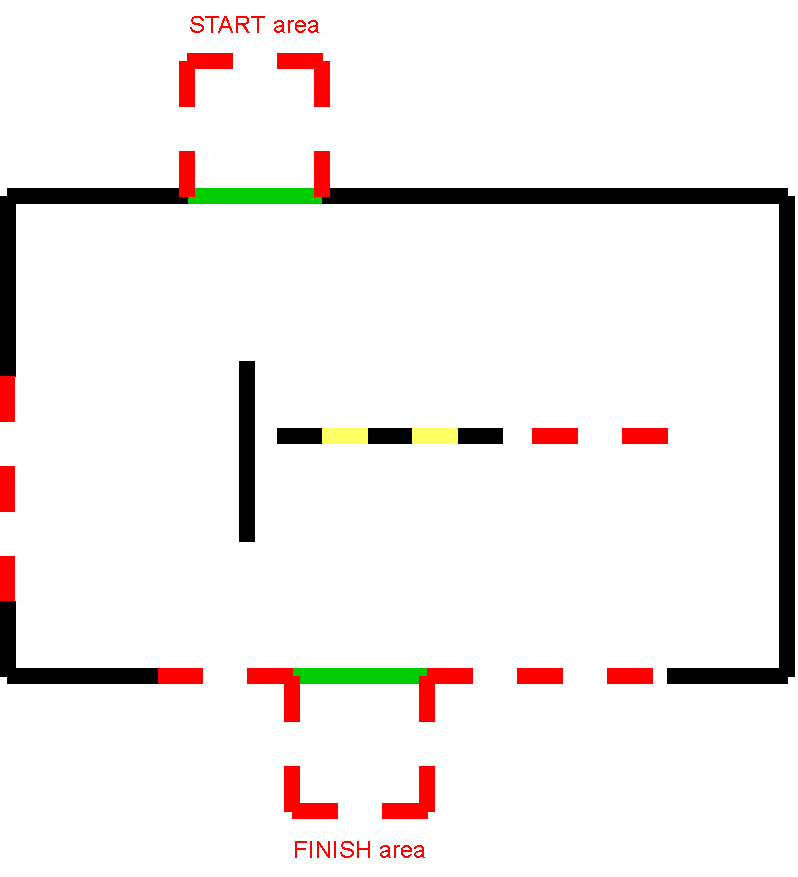
\includegraphics[width= 0.6\linewidth]{./images/arena/tabes.pdf}
	\end{center}
	\caption{Exemplary tape configuration: black lines are physical walls, red white dashed lines are virtual walls, yellow black dashed lines are barrier tape and green lines are marking tape}
	\label{fig:tapeconfig}
\end{figure}




\textbf{Referee Zone}

The arena is enclosed by a padded strip of 1m. This area is reserved for the referees to enable them to move freely while judging a robot's performance. See section \ref{sec: teams and roles}.


\clearpage

\section{Service Areas}
\label{sec:Service_Areas}
A Service Area indicates a location for a robot where tasks (e.g. picking or placing Objects) have to be performed.
\subsection{General} 
\label{subsec:Service_Areas_General}


Such a location is usually a Table with a flat white top (see fig. \ref{fig:arena_example}), commonly referred to as Workstation (only in a case of a normal Table), but can also be a Rotating Table, Shelf, Precise Placement station or any other type needed for a specific task.
In order to successfully reach a Service Area, robots must position themselves in front of the Service Area in a way that allows manipulation of the Objects of interest and the robot has to stand still. To enable robots to reach such a position, a rectangular area with $80\si{\centi\meter}$ width must be kept free of Obstacles (see fig. \ref{fig:arena_service_area_free}). 

\begin{figure} [h!]
	\centering
	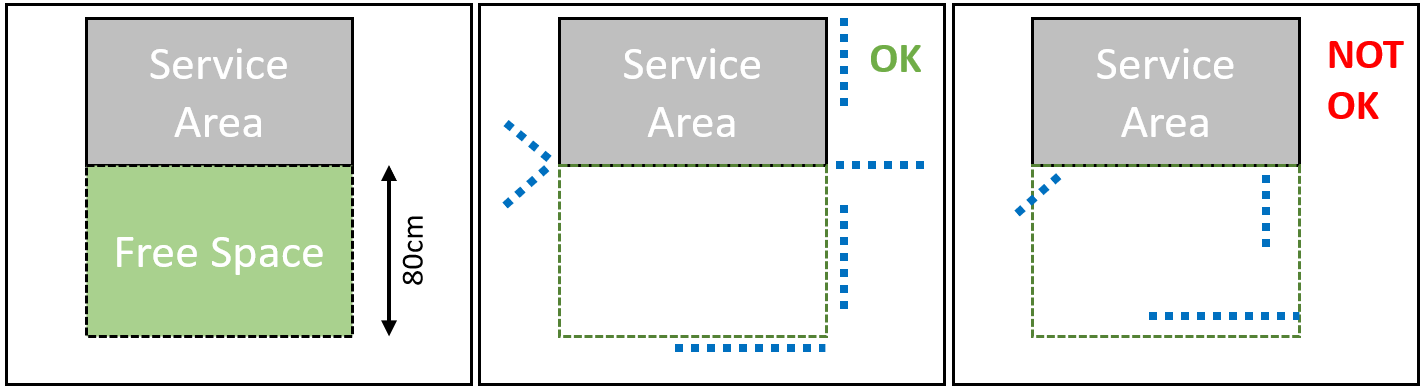
\includegraphics[width= 0.8\textwidth ]{./images/general_rules/arena_service_area_free_space}
	\caption{Free Space in front of a Service Area}
	\label{fig:arena_service_area_free}
\end{figure}

The arena layout must define where the "front" of a table is.
Figure \ref{fig:arena_map_annotated} gives an example for the definition of the position of each Service Area, marking them as WSx (Workstation x), SHx (Shelf x), PPx (Precise Placement x)and RTx (Rotating Table x). The orientation only indicates the direction of the Service Area. It does not specify the robot's heading, which may be chosen by teams according to their individual robot design.

Tables that includes Service Areas which can be used from both sides (see fig. \ref{fig:arena_example}) are defined as two seperate workstations (e.g. WS5 \& WS6). However, manipulation of theses Service Area requires the robot to have its center in the rectangular area defined in fig.~\ref{fig:arena_service_area_free}. This means that manipulation of the opposite Service Area is NOT allowed (see \ref{ssec:ManipulationZone}), even though it would be physically possible.

This rule also applies to the two positions for the Rotating table (RT1 and RT2).
This makes smaller physical layouts possible that still provide the ability to create complex navigation challenges due to the amount of locations to visit.


\subsection{Arbitrary Surfaces and Decoys}
\label{subsec:Arbitrary_Surfaces_and_Decoys}

In order to make the operating environment more realistic, the Service Areas may contain different kinds of Arbitrary Surfaces (Figure \ref{fig:ast_surface_example}) with industrial items as Decoys (Figure \ref{fig:ast_example}). The Decoys are limited in height to max. 10~cm. The width and depth of decoys are only limited by the size of the manipulation area. The Arbitrary Surfaces don't have to be fixed mounted at the Service Areas. Examples of Arbitrary Surfaces can be different wood pattern, grass, alufoil, plexiglas etc. The integration of Arbitrary Surfaces and Decoys into tests is according the table \ref{fig:test_specifications_instance}. If a team choose AprilTag objects in a test then no arbitrary surfaces will be used.


\begin{figure}[h!]
	\centering
	\subfloat[]{\includegraphics[width=.23333\textwidth]{./images/Arbitrary_Surface_rug}}
	\hspace{.05\textwidth}
	\subfloat[]{\includegraphics[width=.23333\textwidth]{./images/Arbitrary_Surface_wood}}
	\hspace{.05\textwidth}
	\subfloat[]{\includegraphics[width=.23333\textwidth]{./images/Arbitrary_Surface_grass}}\\
	\subfloat[]{\includegraphics[width=.23333\textwidth]{./images/Arbitrary_Surface_fake_wood_1}}
	\hspace{.05\textwidth}
	\subfloat[]{\includegraphics[width=.263333\textwidth]{./images/Arbitrary_Surface_fake_wood_2}}
	\caption{Examples of arbitrary surfaces used for Service Areas.}
	\label{fig:ast_surface_example}
\end{figure}

\begin{figure}[h!]
	\begin{center}
		\subfloat[]{\includegraphics[width=.375\textwidth]{./images/realisticWorkingDeskI.jpeg}}
		\hspace{.05\textwidth}
		\subfloat[]{\includegraphics[width=.375\textwidth]{./images/realisticWorkingDeskII.jpeg}}
	\end{center}
	\caption{Examplary configuration of the working desks including objects and decoys.}
	\label{fig:ast_example}
\end{figure}

Placement of Decoys and arbitrary surfaces are done by the referees. Decoys could be any kind of object (tools, hardware, small electrical devices) but also standard objects from the rule book defined in section~\ref{ssec:ManipulationObjects} can be used. Figure~\ref{fig:ast_example} shows some examples. 



\subsection{Containers}
\label{subsec:containers}
As in many industrial settings, the \RCAW environment may be equipped with several Containers (see Figure~\ref{fig:containers}). The Containers are defined as industrial plastic stacking boxes size 2B, outer dimensions: $135 \times 160 \times 82  \si{\milli\meter}$, usable dimensions: $120 \times 125 \times 65  \si{\milli\meter}$  in red ca. RAL 3020 and blue ca. RAL 5015.
% \href{https://www.amazon.de/gp/product/B0062TUUOE/ref=ppx_yo_dt_b_asin_title_o01_s00?ie=UTF8&psc=1}{example Container from amazon} (visited Januar 2022). 
They can store any kind of Object defined in Section~\ref{ssec:ManipulationObjects}. Robots are supposed to place previously grasped Objects into containers. 
(Grasping from containers might be included in future competitions.) Several Containers can be present in the environment and are always associated with a Service Area. That means that the Container itself will be placed within the manipulation zone defined in Section~\ref{ssec:ManipulationZone}.
It is also possible that more than one Container is placed at a single Service Area, but not multiple Containers of the same color.
The constraints defined in Section~\ref{ssec:ManipulationZone} apply also to the Containers.
Currently, a Container itself does not need to be manipulated or transported by the robot. The position of the Containers will be decided by the referees before every run type.

\begin{figure} [h!]
	\begin{center}
		\subfloat[blue]{\includegraphics[width= 0.375\textwidth]{./images/container_blue.jpg}} 
		\hspace{0.05\textwidth}
		\subfloat[red]{\includegraphics[width= 0.375\textwidth]{./images/container_red.jpg}}
	\end{center}
	\caption{Containers can be used for grasping Objects out or placing Objects into them.}
	\label{fig:containers}
\end{figure}


\section{Objects} 
\label{ssec:ManipulationObjects}

The Objects in \RCAW include a wide range of Objects relevant in industrial applications of robotics. They eventually cover any raw material, (semi-)finished parts or products as well as tools and possibly operating materials required for manufacturing processes. Object types are selected by the TC and shall vary in complexity due to different shapes, colors and uses of objects. Currently there are three sets of Objects used in the competition: Basic, Advanced and April Tagged. The following sections provide details about those sets. The exact appearance of the object used in the competition can slightly vary due to availability, e.g. different coating colors for some standard parts.



%TODO: Still need this or can we remove it with introduction of new object set?
%
%Additionally, a set of so called RoCKIn objects is used in the competition (see table~\ref{tab:manipulation_objects_rockin}). 
%These parts build a drive train of a KUKA youbot and might be used for assembly tasks.
%\textbf{REMARK:} Due to poor availability of the original RoCKin object set, teams are allowed to to use a set of 3D printed copies. The material used for fabrication has to be in standard grey/silver colour using fine quality settings and PLA as printing material. 
%An example is given with PLA Silver (ca. RAL 9006), thickness 1.75 or 2.85, not specified in detail.

%\href{https://www.amazon.de/-/en/TINMORRY-1-75mm-Filament-Printer-Spool/dp/B089YX78N5/ref=sr_1_6?crid=ZTL2O0EL3B3B&keywords=pla%2Bfilament%2Bgrau%2Bral%2B9006&qid=1641982915&s=industrial&sprefix=pla%2Bfilament%2Bgrau%2Bral9006%2Cindustrial%2C114&sr=1-6&th=1 }{example material from amazon} (visited Januar 2022). 
%Figure~\ref{fig:RoCKIn_printed} shows an example set of the printed RoCKIn Objects created using fused filament fabrication (FFF) printing. 


% as shown in  and . Objects of one kind can slightly vary e.g. considering the surface and coating colour. 

%RoCKIn Objects are spare parts from the KUKA you-bot platform often used in the competition, due to the fact that the KUKA you-bot and the RoCKIn Objects are not longer produced in future those Objects will be replaced with other standard parts used in industry as shown in Section~
%\ref{sec:new_objects}. 


\subsection{Basic Object Set}

The Basic Object Set includes standard profile rails, screws and nuts with various sizes and masses.
% (see table~\ref{tab:manipulation_objects}).

\newcommand{\imageView}[1]{\includegraphics[width=2cm, valign=c]{#1}}
\newcommand{\rowpadding}{0.4cm}
\setlength\extrarowheight{\rowpadding}


\begin{table}[h!]

\begin{tabular}{|c|c|c|c|m{8cm}|}
\hline
ID & Object & Symbolic Description & Mass & Details \\
\hline

\texttt{1} & \imageView{./images/F20_20_B.jpg} & \texttt{F20\_20\_B} & 49 g & Small aluminium profile \newline
 Coating/Colour: black anodized\newline
 Size: $20 \times 20 \times 100 mm$ \\ [\rowpadding]
\hline

\texttt{2} & \imageView{./images/F20_20_G.jpg} & \texttt{F20\_20\_G} & 49 g & Small aluminium profile \newline
 Coating/Colour: gray anodized\newline
 Size: $20 \times 20 \times 100 mm$ \\ [\rowpadding]
\hline

\texttt{3} & \imageView{./images/S40_40_B.jpg} & \texttt{S40\_40\_B} & 186 g & Large aluminium profile\newline
 Coating/Colour: black anodized\newline
 Size: $40 \times 40 \times 100 mm$ \\ [\rowpadding]
\hline

\texttt{4} & \imageView{./images/S40_40_G.jpg} & \texttt{S40\_40\_G} & 186 g & Large aluminium profile \newline
 Coating/Colour:  gray anodized\newline
 Size: $40 \times 40 \times 100 mm$ \\[\rowpadding]
\hline

\texttt{5} & \imageView{./images/M20_100.jpg} & \texttt{M20\_100} & 296 g & Screw\newline
 ISO4014, DIN 931, EU 24014 \newline
 Coating/Colour: blank, black burnished \newline
 Size: M$20\times 100$ \\ [\rowpadding]
\hline

\texttt{6} & \imageView{./images/M20.jpg} & \texttt{M20} & 56 g & Small nut\newline
 ISO4032, DIN934, EU 24032  \newline
 Coating/Color: blank, black burnished \newline
 Size: M20 \\ [\rowpadding]
\hline

\texttt{7} & \imageView{./images/M30.jpg} & \texttt{M30} & 217 g & Large nut\newline
 ISO4032, DIN934, EU 24032  \newline
 Coating/Color: blank, black burnished \newline
 Size: M30 \\ [\rowpadding]
 \hline
\end{tabular}
\caption{\RCAW Basic Object Set}
\label{tab:manipulation_objects}
\end{table}



\clearpage
%\subsection{RoCKIn Object Set}
%
%\subsubsection{Original Set}
%
%
%\begin{table}[h!]
%\begin{tabular}{|c|c|c|c|m{6cm}|}
%\hline
%ID & Object & Symbolic Description & Mass & Details \\
%\hline
%
%\texttt{8} & \imageView{./images/bearingBoxA.jpg} & \texttt{Bearing\_Box} & 102 g & Bearing box\newline
% Height: 25 mm \newline
% Width: 45 mm \newline
% Length: 50 mm \newline
% Inner diameter: 32 mm \\ [\rowpadding]
%\hline
%
%\texttt{9} & \imageView{./images/bearing.jpg} & \texttt{Bearing} & 42 g & Bearing\newline
% Height: 13 mm \newline
% Inner diameter: 15 mm \newline
% Outer diameter: 32 mm \\ [\rowpadding]
%\hline
%
%\texttt{10} & \imageView{./images/axis.jpg} & \texttt{Axis} & 40 g & Axis\newline
% Diameter: 27 mm \newline
% Length: 96 mm \\ [\rowpadding]
%\hline
%
%\texttt{11} & \imageView{./images/distanceTube.jpg} & \texttt{Distance\_Tube} & 5 g & Distance tube\newline
% Height: 10 mm \newline
% Inner diameter: 28 mm \newline
% Outer diameter: 32 mm \\ [\rowpadding]
%\hline
%
%\texttt{12} & \imageView{./images/motor.jpg} & Motor & 20 g & Motor\newline
% Diameter: 42 mm \newline
% Length: 87 mm \\ [\rowpadding]
%\hline
%
%\texttt{13} & \imageView{./images/R20.jpg} & \texttt{R20} & 14 g & Plastic tube\newline
%Inner diameter: 20 mm \newline
%Outer diameter: 30 mm \newline
%Length: 45 mm \\ [\rowpadding]
%\hline
%%\imageView{./images/V20.jpg} & \texttt{V20} & 14 g & Inner diameter: 20 mm \newline
%%Outer diameter: 30 mm \newline
%%Length: 45 mm \\
%%\hline
%\end{tabular}
%\caption{RoCKIn Object set.}
%\label{tab:manipulation_objects_rockin}
%\end{table}
%}
%
%\clearpage
%\subsubsection{Printed Set}
%
%
%\begin{figure}[h!]
%	\begin{center}
%		\subfloat[]{\includegraphics[width=0.8\textwidth]{./images/rockingPrinted1.jpg}}
%		\vspace{0.05\textwidth}
%		\subfloat[]{\includegraphics[width=0.8\textwidth]{./images/rockingPrinted2.jpg}}
%	\end{center}
%	\caption{Examplary 3D printed RoCKIn Objects (bearing box, bearing, axis, distance\_tube, motor, plastic tube R20). Material:  PLA silver ( ca. RAL 9006), 2.85mm. Printer: Ultimaker 3 extended. Printer settings: fine}
%	\label{fig:RoCKIn_printed}
%\end{figure}



\clearpage
\subsection{Advanced Object Set}


For 2023, the RoCKIn object set (see 2022 rulebook or previous ones) is replaced by a selection of better available parts for a drive train, as well as some tools (see Section~\ref{sec:new_objects}). The new object set was introduced in a technical challenge in 2022 and is called Advanced Object Set.

\begin{table}[h!]
	\begin{tabular}{|c|m{2cm}|c|c|m{8cm}|}
		\hline
		ID & Object & Symbolic Description & Mass & Details \\
		\hline
%%%%%%%%%%%%%
		\texttt{20} & \imageView{./images/newObjects/welle3d.jpg} \newline
		\imageView{./images/newObjects/welleSchematic.JPG}
		& \texttt{Axis2} & 180 g & Steel axis \newline
		Misumi: SFUB25-25-F28-P17-T15-S10-Q20 \newline
		Coating/Colour: blank, black burnished \newline
		Length: 68 mm \newline
		Diameter: 17mm, M20 \newline
		%see Figure~\ref{fig:welle2Schematic} \newline
		
		\href{https://de.misumi-ec.com/vona2/detail/110302635710/?CategorySpec=00000146753%3a%3ab%2cc}{Misumi} (visited Januar 2022)\\

			\hline
%%%%%%%%%%%%
		\texttt{21} & \imageView{./images/newObjects/bearing2.JPG} & \texttt{Bearing2} & 100 g & Bearing \newline 
		SKF YAR203-2F\newline
		Coating/Colour: gray \newline
		Useable with housing\newline
		\href{https://www.skf.com/sg/products/rolling-bearings/ball-bearings/insert-bearings/productid-YAR%20203-2F}{SKF}  (visited Januar 2022)\\
		\hline
%%%%%%%%%%%%				
		\texttt{22} & \imageView{./images/newObjects/housing.JPG} & \texttt{Housing} & 60 g & Housing \newline 
		SKF P40\newline
		Coating/Colour: gray \newline
		Useable with bearing\newline
		\textbf{Remark:} needs two hex socket screw M8x10 (ISO 4762, DIN 912) and two M8 nuts (ISO 4032, DIN 934) \newline
		\href{https://www.skf.com/sg/products/mounted-bearings/ball-bearing-units/pillow-block-ball-bearing-units/productid-P%2040}{SKF}  (visited Januar 2022)\\
		\hline
%%%%%%%%%%%%	
		\texttt{23} & \imageView{./images/newObjects/motor.JPG} & \texttt{Motor2} & 350g & Motor 755\newline
		Coating/Colour: gray \newline
		Size: $66.7 \times 42.0 \si{\milli\meter}$\newline
		Diameter: $d_{axis}=5\si{\milli\meter}$, $l_{axis}=10\si{\milli\meter}$ \newline
		\href{https://www.amazon.de/EsportsMJJ-12V-36V-3500-9000Rpm-Drehmoment-Hochleistungsmotor/dp/B075D85KVV}{Amazon}  (visited Januar 2022)\\
		\hline
%%%%%%%%%%%%					
		\texttt{24} & \imageView{./images/newObjects/FlangedResinCollar.JPG} & \texttt{Spacer} &  & Flanged Spacer\newline
		Misumi CLJHJ25-30-70  \newline
		Coating/Colour: white \newline
		Size: $70\si{\milli\meter}$\newline
		Diameter: $d_{inner}=25\si{\milli\meter}$, $d_{outer}=30\si{\milli\meter}$ \newline
		\href{https://us.misumi-ec.com/vona2/detail/110300236450/?curSearch=%7b%22field%22%3a%22%40search%22%2c%22seriesCode%22%3a%22110300236450%22%2c%22innerCode%22%3a%22%22%2c%22sort%22%3a1%2c%22specSortFlag%22%3a0%2c%22allSpecFlag%22%3a0%2c%22page%22%3a1%2c%22pageSize%22%3a%2260%22%2c%2200000042362%22%3a%22mig00000001500952%22%2c%2200000042368%22%3a%22b%22%2c%22jp000157843%22%3a%22mig00000000344081%22%2c%22jp000157846%22%3a%22mig00000001417174%22%2c%22jp000157851%22%3a%22mig00000000344088%22%2c%2200000334029%22%3a%2230%22%2c%2200000334032%22%3a%2270%22%2c%22typeCode%22%3a%22CLJHJ%22%2c%22fixedInfo%22%3a%22MDM0000085422111030023645020110476153310093415426696895%7c14%22%7d&Tab=preview}{Misumi}  (visited Januar 2022)\\
						\hline

\end{tabular}
\caption{Advanced Object Set - Part 1}
\label{tab:new_objects1}
\end{table}


\begin{table}[h!]
	\begin{tabular}{|c|m{2cm}|c|c|m{8cm}|}
		\hline
		ID & Object & Symbolic Description & Mass & Details \\
		\hline
		%%%%%%%%%%%%
		\texttt{25} & \imageView{./images/newObjects/weraScrewdriver.jpg} & \texttt{Screwdriver } & 19g & WERA 352 \newline
		Ball end screwdriver,hexagon socket screws\newline
		Coating/Colour: black/green \newline
		Size: $181\si{\milli\meter}$\newline
		Diameter: $d_{tip}=2.5\si{\milli\meter}$\newline
		Code: 05138070001\newline
		\href{https://www.amazon.de/Wera-05138070001-352-Sechskant-Kugelkopf-Schraubendreher-2-5/dp/B00154ZWFI?th=1}{Amazon}  (visited Januar 2022)\\
		\hline
		%%%%%%%%%%%%			
		\texttt{26} & \imageView{./images/newObjects/weraWrench.jpg} & \texttt{Wrench } & ca. 72g & WERA Jocker 6000, 8mm \newline
		Ratcheting combination wrenches\newline
		Coating/Colour: silver/grey/pink \newline
		Size: ca. $144\si{\milli\meter}$\newline
		Diameter: $d_{max}=20\si{\milli\meter}$\newline
		Code: 05073268001\newline
		\href{https://www.amazon.de/Wera-05073268001-Joker-Maul-Ringratschen-Schl%C3%BCssel/dp/B00BT0GBMG?th=1}{Amazon} (visited Januar 2022)\\
		\hline
		%%%%%%%%%%%%
		\texttt{27} & \imageView{./images/newObjects/hsscoDIN338metaldrill.jpg} & \texttt{Drill } & ca. 10g & Bosch Drill HSS-Co DIN338  \newline
		Drill\newline
		Coating/Colour: gold/ Cobalt alloy \newline
		Length: ca. $151\si{\milli\meter}$\newline
		Diameter: $d_{max}=13\si{\milli\meter}$\newline
		Code: 3165140382724 \newline
		\href{https://www.amazon.com/Bosch-2609255086-Metal-Drill-HSS-Co/dp/B0071OSFQY}{Amazon} (visited Januar 2022)\\
		\hline
		%%%%%%%%%%%
		\texttt{28} & \imageView{./images/newObjects/weraAllenKey.jpg} & \texttt{AllenKey } & ca. 10g & Wera Allen Key 8mm,\newline
		3950 PKL L-key, metric, stainless\newline
		Coating/Colour: silver \newline
		Length: ca. $195\si{\milli\meter} \times 37\si{\milli\meter}$\newline
		Diameter: $d_{max}=8\si{\milli\meter}$\newline
		Code: 05022708001 \newline
		\href{https://www.amazon.co.uk/Wera-WER022708-Hexagon-Keys-Multi-Colour/dp/B00A8QXTNG}{Amazon} (visited Januar 2022)\\
		\hline
		%%%%%%%%%%%
	
\end{tabular}
\caption{\RCAW Advanced Object Set - Part 2}
\label{tab:new_objects2}
\end{table}

\clearpage


\subsection{April Tagged Object Set}
\label{ssec: April Tagged Object Set}

For the season 2023 and onwards, 3D printed cubes marked with April tags might be used in the competition. 
This should allow teams to focus on other areas than object recognition by simplifying the detection of Objects. 
These cubes will be called April Tag Tagged Cubes (ATTC) in the following.

The April Tags used in \RCAW measure $40 \si{\milli\meter} \times 40 \si{\milli\meter}$ and have an encoding taken from the \textit{36h11} April Tag family, including a 1bit black and 1bit white border as shown in fig. \ref{fig:singleAprilTag}. 


\begin{figure}[h!]
	\centering
	\includegraphics[width= 0.4\textwidth ]{./images/singleAprilTAG42.png}
	\caption{Example of an April Tag with the ID 42. Encoding is from the 36h11-April Tag Family.}
	\label{fig:singleAprilTag}
\end{figure}

All the used April Tag ID numbers will fit to the ID numbers used by the AtWork Commander in the \href{https://github.com/robocup-at-work/atwork-commander/blob/master/atwork_commander_msgs/msg/Object.msg}{atwork\_commander\_msgs/msg/Object.msg}. 

Any software package to identify such april tags is allowed. The \href{http://wiki.ros.org/apriltag_ros}{April Tag ROS package} would be a great and easy-to-use example.


%
%uint16 EMPTY = 0
%
%# atwork
%uint16 ATWORK_START = 11
%uint16 F20_20_B = 11
%uint16 F20_20_G = 12
%uint16 S40_40_B = 13
%uint16 S40_40_G = 14
%uint16 M20_100 = 15
%uint16 M20 = 16
%uint16 M30 = 17
%uint16 R20 = 18
%uint16 ATWORK_END = 19
%
%# rockin
%uint16 ROCKIN_START = 21
%uint16 BEARING_BOX = 21
%uint16 BEARING = 22
%uint16 AXIS = 23
%uint16 DISTANCE_TUBE = 24
%uint16 MOTOR = 25
%uint16 ROCKIN_END = 26
%
%# container
%uint16 CONTAINER_START = 31
%uint16 CONTAINER_RED = 31
%uint16 CONTAINER_BLUE = 32
%uint16 CONTAINER_END = 33
%
%# cavity
%uint16 CAVITY_START = 41
%uint16 F20_20_H  = 41
%uint16 F20_20_V  = 42
%uint16 F20_20_F  = 43
%uint16 S40_40_H  = 44
%uint16 S40_40_V  = 45
%uint16 S40_40_F  = 46
%uint16 M20_H     = 47
%uint16 M20_V     = 48
%uint16 M20_F     = 49
%uint16 M20_100_H = 50
%uint16 M20_100_V = 51
%uint16 M20_100_F = 52
%uint16 M30_H     = 53
%uint16 M30_V     = 54
%uint16 M30_F     = 55
%uint16 R20_H     = 56
%uint16 R20_V     = 57
%uint16 R20_F     = 58
%uint16 CAVITY_END = 59 


\subsubsection{Dimensions and Details of the ATTCs}

The standard ATTC measures $42\si{\milli\meter} \times 42\si{\milli\meter} \times 42 \si{\milli\meter}$ and has slightly rounded edges, similar to the shape of aluminum profile rails. 
A $1\si{\milli\meter}$ deep cavity measuring $40.5\si{\milli\meter} \times 40.5\si{\milli\meter}$ is embedded in the top of the cube to make centering the april tag printouts easier.
The exact design and size is specified in fig. \ref{fig:cubeObject} and can be downloaded from the official league repository: \href{https://github.com/robocup-at-work/rulebook/tree/alpha_2023/images}{3D STL file for an ATTC}

\begin{figure}[h!]
	\centering
	\subfloat[April Tag Tagged Cube (ATTC), including overall dimensions.]{\includegraphics[width=0.375\textwidth ]{./images/AprilTags/AprilTagCube2023_2.png}}
	\hspace{0.05\textwidth}
	\subfloat[Detailed dimensions of the ATTC cavaty to fix a certain April Tag.]{ \includegraphics[width=0.375\textwidth ]{./images/AprilTags/AprilTagCube2023_1.png} }
	\caption{3D construction of the ATTC as manipulation object.}%
	\label{fig:cubeObject}
\end{figure}

The cubes are 3D printed using PLA filament. Any color is allowed since the identification of cubes is solely done using the printout tag, which is to be glued into the top cavity.
Additionaly, printouts of a human-readable object ID and an image of the corresponding object from tables \ref{tab:manipulation_objects}, \ref{tab:new_objects1} and \ref{tab:new_objects2} must be glued to the side of the cubes to allow for easier onsite handling and identification of the cubes.

\begin{figure}[h!]
	\begin{center}
		\subfloat{\includegraphics[width=0.32\textwidth,rotate=-0]{./images/AprilTags/AT_obj_1.jpg}} \hfill
		\subfloat{\includegraphics[width=0.32\textwidth,rotate=-0]{./images/AprilTags/AT_obj_2.jpg}} \hfill
		\subfloat{\includegraphics[width=0.32\textwidth,rotate=-0]{./images/AprilTags/AT_obj_3.jpg}} \hfill
	\end{center}
	\caption{Examples of allowed ATTCs}
	\label{fig:real ATTCs}
\end{figure}



\subsubsection{Tagged Targets}

To allow for the more advanced tasks to be performed using the simplified april tag detection method, the target objects (precise placement cavities and containers) are also marked with a tag.

Containers are marked with a tag glued to the inside bottom of the container. The tag shall be placed as centered as possible.

For the precise placement tests, a special PP tile is used which allows a tag to be placed with a constant offset from the hole (see fig. \ref{fig:Tagged Targets}). The used ID matches the ID of the object that must be placed into that cavity.

\begin{figure}[h!]
	\begin{center}
		\subfloat{\includegraphics[width=0.32\textwidth,rotate=-0]{./images/AprilTags/AT_Container.jpg}} \hfill
		\subfloat{\includegraphics[width=0.32\textwidth,rotate=-0]{./images/AprilTags/CubeTile2023_2.png}} \hfill
		\subfloat{\includegraphics[width=0.32\textwidth,rotate=-0]{./images/AprilTags/CubeTile2023_1.png}} \hfill
	\end{center}
	\caption{Examples of tagged targets}
	\label{fig:Tagged Targets}
\end{figure}




\subsection{Manipulation Zone} \label{ssec:ManipulationZone}
The manipulation zone defines the area where Objects can be placed. Thereby, the following constraints need to be satisfied:
\begin{itemize}
	\item The maximum depth of the manipulation zone from the front of the service area to the end of the manipulation zone is $20\si{\centi\meter}$.
	\item The minimum distance between Objects to each other is $2\si{\centi\meter}$.
	\item The minimum distance of the beginning of the manipulation zone to a Wall is $10\si{\centi\meter}$.
	\item There as an offset of $2\si{\centi\meter}$ from the border of the Service Area to the manipulation zone.
\end{itemize}
Note, the constraints do not permit, that Objects can be partially occluded dependent on the viewpoint.

For the placement of Objects the following terms are used:

\begin{itemize}
	\item Position: point within 2D coordinate system of a Manipulation Zone,
	\item Rotation: rotation around vertical axis of a Manipulation Zone,
	\item Orientation: rotation around horizontal axes of a Manipulation Zone, i.e. whether the Object is standing upright or lying on its side
	\item Pose: combination of position, rotation and orientation.
\end{itemize}
\begin{figure} [h!]
	\centering
	\includegraphics[width=0.8\textwidth ]{./images/manipulation_zone2023.pdf}
	\caption{Manipulation zone: the green color indicates the area where Objects can be placed on a Service Area by the referees.}
	\label{fig:manipulation_zone}
\end{figure}











\chapter{Competition}
% !TEX root = ../Rulebook.tex
\label{sec:Competition}

\section{Teams and Roles}
\label{sec: teams and roles}

The TC and OC will jointly determine the number of teams permitted to participate in a competition well in advance. The rules shall enable a competition with up to at least 24 teams lasting not more than four full days. The number of people to register per team is not restricted by default, but may be limited due to local arrangements. Teams that plan to bring more than four members are advised to contact the OC beforehand.

During registration, each team has to designate one member as teamleader. A change of the teamleader must be communicated to the OC. 
The teamleader is the only person who can officially communicate with the referees during the competition, e.g. aborting a run, to call a restart, etc. 
The teamleader may ask the OC to accept additional teammembers for these tasks.

Each team must also nominate one person which acts as a referee during all tests.
The job of each referee is to ensure that the arena state before each performance is the same as the initial run setup.
They also rate the robot performances during a run. 
This ensures that the interests of every team are respected equally.
It also involves the refs in discussions with other teams and the league officials,
which helps getting to know each other.
Each referee gets a referee sheet from the OC which is used to evaluate the performance. An additional referee is the head referee which measures the time and organizes the referees. If less than 4 referees without the head referee are available (so less than 4 teams participate), TC members can also be referees to fill this up to 4. 4 referees are beneficial, because there is at least one on each side of the arena. A referee briefing is held before a competition by the TC and OC. The goal is to discuss questions and to sensitize the referees for their task. Only briefed refs are allowed to judge the future runs. Teams are asked to send at least two members to the briefing, if possible.

Teams are asked (and wished) to comment their robots performance during their run.
This makes the competition more entertaining while also sharing knowledge about robots, 
the challenges of a task and smart solutions.
The commentator may be any teammember and is optional during competitions.

\section{Meetings and Language of Communication}

Both the TC and the OC may organize several special meetings during a competition, 
such as referee meetings, teamleader meetings, etc.
The meetings are held in english and will be planned and announced locally.
They are used to clarify rules, assign timeslots, request test participation or for any other exchange of information between teams and commitee members.
It is the responsibility of each team to inform themselves about the organization and scheduling of such meetings.
Each team is expected to send at least one representative to such meetings. If the meeting refers to specific roles, such as 'referee' or 'team leader', the person designated by the team to fill this role is expected to participate.


\section{Code of Conduct and Disqualification}
Teams and team members are expected to maintain a friendly and cooperative atmosphere throughout a competition and contribute to a vivid work environment and to scientific exchange before, during and after a competition.
\par
The TC may disqualify individual team members or a whole teams during a competition for severe reasons, such as repeated breach of rules.


\section{Competition Procedure}

The competition is held in the form of so called tests.
A test requires a robot to perform various abilities, including navigation, manipulation, task planning and autonomous decision making.
Different kinds of tests each have their focus a current research field, e.g. picking moving objects or efficient task execution.

All tests require a robot to autonomously navigate through the arena defined in \ref{sec:ArenaDesign} without causing a collision. Each team can enter the arena before actual competitions to create a map of the environment and test their robot. The OC will organize time slots for each team respecting the amount of teams and available slots. Usually there will be some setup days that can be used only for training.

\section{Time Schedule}

The actual competition currently includes a total of 7 tests.
These are spread across available competition days with time buffers in between each other.
An example for the schedule can be found here: \url{https://atwork.robocup.org/rc2021/}.
As on site events have tighter schedules and additionally require teams to prepare everything for an unknown environment, there will usually be two setup days before the four competition days.
Nonetheless, Teams should expect things to be a bit stressful and prepare for something like fig. \ref{fig:example_schedule}.

\begin{figure}[h!]
\centering
\includegraphics[width= 0.9\textwidth ]{./images/competition/Competition_Schedule_2024}
\caption{Example of a time schedule for a \RCAW competition.}
\label{fig:example_schedule}
\end{figure}


\section{Practice Slots}

The teams will be given an opportunity to practice with their robots either in the competition arenas or in special test arenas, if available. The frequency and lengths of practice periods will be decided by the OC on site. The OC will also decide about if and how many teams may use an arena simultaneously and can decide on a practice schedule for teams wishing to use the arenas. Arenas may be modified between practice time and competition runs.

\section{Teamleader Meetings}

During a comptetition, the TC and/or EC usually have some points to discuss with all teamleaders regarding onsite organization, rule clarification, agreements on onsite-test-procedures and similar topics.
The schedule includes two dedicated slots each day for such called TeamLeader Meetings (TLM), which may be used by the TC/EC if necessary.
All teamleaders are required to attend those meetings.


\section{Qualification for a Test}
\label{sec:qulaification for a test}

Depending on the amount of participating teams and available timeslots, 
the competition \textbf{may be} seperated into different stages.
Starting with the rather easy tests including all teams, only high performing teams might be allowed to participate in later (more difficult) tests.

The OC must create an onsite schedule during the setup days and announce it before the first competition day. 
The schedule should include all teams in all tests if possible,
but might introduce special stages in the following order:
\begin{enumerate}
\item Stage One: limit the maximum amount of teams in the final test, only the X best teams may participate
\item Stage Two: limit the maximum amount of teams in the Advanced Transportation and later tests, only the X best teams may participate
\end{enumerate}

Teamleaders of qualified teams are required to announce 1 hour before the respective time slot wether their team likes to participate in a test or not. 
This enables the OC to plan the schedule and create scoring sheets.

\section{Parc ferm\'e}

All participating teams must bring their performing robot to the parc ferm\'e 15 minutes before a test and leave them there during the whole timeslot of the test, except when they must perform.
Rules similar to motorsports apply: The robot must not be worked on or changed in any kind unless
serious damage must be repaired. This intends to encourage teams to watch other performances while still give teams the chance to remain in the competition. It is allowed to attach a charger to the robot.

The location of the parc ferm\'e will be towards the spectators for entertainment.
The robots may (are wished to) be turned on and ready to perform, enabling teams to set robot arm positions and illumination for the visitors. 

If the power management of a robot does not enable it to be turned on during the runs of other teams,
the specific team may power-on and boot their robot once the run of the previous team has ended.
They may not change or modify their robot in any way during this time (hardware and software).

\section{Test Procedure}

15 minutes before a competition slot, the arena is set up for the upcoming test.
Therefore, the position of each static arena element is checked and objects are placed on active 
Service Areas.
The TC will decide where dynamic arena elements are placed. See table \ref{fig:test_specifications_instance} for the different responsibilities of placing arena elements, Objects (Pose), Decoys, Containers etc.

A competition slot consists of multiple performance slots (one for each team), 
including a preparation phase, the run phase and the end phase.

\textbf{Preparation Phase}

During the prep phase, teams are allowed to move their robot from the parc ferm\'e to the defined start pose in the arena either by hand or by carefully driving manually. They should prepare their robot for their run and can therefore remote access the robot and/or make minor changes.
It is explicitly forbidden to hardcode solutions for specific requirements of a test during this phase (e.g. drawing position of obstacles in the map). Also, if the robot passes and detects obstacles during this phase, they must be erased from the memory (e.g. clear costmap) unless they can be detected from the START location. The TC might disqualify teams that try to gain unfair advantages from the current or even the following tests.



\textbf{Run Phase}

The run phase begins once the preparation time is up or when the teamleader announces that the team is ready. 
The task is then sent to the robot and from there on, the robot must act fully autonomously. 
It is forbidden to interact or control the robot in any human kind (keyboard/mouse actions, gestures, voice). 
The only interaction allowed is the unplugging of a LAN cable connecting the robot and the controlling pc
when relying on wired communication due to onsite WiFi jams.

During the run phase, the robot must not leave, nor may any person enter the arena.
Teammembers of the performing team are allowed to enter the arena to prevent damage in case of an error (e.g. remove a dropped object from the robots path), but receive a penalty for each interaction.
If a robot behaves uncontrolled and poses a potential threat to the environment,
any person may approach the robot and press the emergency stop.
However, it is requested and strongly advised that only the developers touch their robot.


The run phase regularly ends when:
\begin{itemize}
\item The robot has reached the FINISH location of the arena
\item The run time is up
\item The teamleader says 'stop'
\end{itemize}

The run phase ends early when:
\begin{itemize}
\item The robot has caused a second major collision
\item The emergency stop button had to be pressed before a restart call
\item A team was identified to be cheating 
\end{itemize}

The end of a run phase must be announced by the OC by saying 'end'.
Once this happened, the team may touch and control their robot to bring it to a full stop.

\textbf{End Phase}

In the resulting end phase the team is expected to move their robot back to parc ferm\'e.
Referees gather and discuss their performance rating afterwards.
Once they agree on the performing team's result, 
the teamleader is required to accept this score. 
Teams are allowed to make their case if they do not agree with the refs decision,
but cannot force changes and are expected to be understanding.
Special cases will be decided by the TC if the rulebook leaves room for interpretation.

Once the score has been accepted by a team,
the arena must be set up for the next run if necessary.
The prep time of the next team begins once the arena state is declared as ready by all refs.


\textbf{Performance Slot Example}

\begin{figure} [h!]
	\begin{center}
		\includegraphics[width= 0.9\linewidth]{./images/competition/performance_slot}
	\end{center}
	\caption{Performance Slot Example: each team gets one per test, following the random team order}
	\label{fig:performance slot example}
\end{figure}



\section{Restarting a Run}
\label{sec:restartingarun}

During a run, the teamleader can restart the test execution once.
Therefore he/she must say 'restart', which stops the current run phase. The robot must be stopped using the emergency switches, which then allows the refs to reset the arena state.
The remaining run time will be noted and used after the restart. Once the refs have finished resetting the arena, the performing team is brought back to their prep phase, which allows them to move the robot back to the start area and prepare it for the restarted run.
A so called tactical call of a restart (e.g. to prevent a major collision) is allowed, because this rewards the teams knowledge about the robot.
Note: When the first major collision occurs, the team can decide whether they stop the run or they restart the run (see section \ref{sec:Collisions}).


\section{Skipping Tests}

If a team decides to not participate in a test during the official time slot, 
they may repeat that test type once in one of the following competition slots.
Their performance slot for the later test type is then replaced by one that suits the previously skipped test type, 
and they then can perform that test type instead of the originally scheduled one.

This should enable struggling teams to do the more simpler tests later in the competition,
but should only be used by teams if it is really necessary in order to keep the structure of the overall competition. 
It is not allowed to repeat a test that has been replaced with this option.

Please note that this option might not be available at all if the schedule is too tight otherwise.

\section{Atwork Commander (AC)}
\label{sec:atwork-commander}

All specific test configurations are being generated using the atwork-commander.

\begin{center}
	\url{https://github.com/robocup-at-work/atwork-commander}
\end{center}

The purpose of the atwork-commander is to create randomized test configurations for any given arena configuration.
It thereby essentially functions as a master control, creating and sending current tasks to robots.
It may also keep time during the prep, run and end phase.
Robots must connect to the atwork-commander using one of the following interfaces:

\paragraph{Object Scoped}
The commander generates transportation tasks for each individual object that must be transported.
This includes the object class and the initial and target service area.
The exact pose of the object is not specified and the order of all transportation tasks is random.

\paragraph{Arena Scoped}
The commander transmits the initial and the target state of the arena.
Service areas each contain the respective objects according to the individual test configuration,
meaning robots must figure out the transportation tasks by themselves.

Robots should remain connected to the AC during their whole test run.
It may be required (optional) to send feedback to the AC (heartbeat, completed tasks).
Please access the github for detailed interface desciptions.

\subsection{On Site}

During a robocup, one unique test configuration is created and being used for each individual test.
All teams must perform this (the same) test configuration in their assigned performance slot.
For training purposes, other configurations may be created and sent to a robot during a test slot of the team.

Depending on the organization and possibilities on site, the TC must either provide all teams with atleast one "public" PC with a running AC to allow them to test their connection setup or decide before the first competition day if only bagfiles are being used.

In this case, robots do not have to connect to the atwork commander during a run, but may rather process the contents of the rosbag and start the task execution.
The run phase of a team then starts once the robot operator announces his starting action (executing a 'rosbag play NAME' command). 





\chapter{Tests}
% !TEX root = ../Rulebook.tex
\label{sec:Tests}

\section{General}

\subsection{Common Rules}
\label{ssec: Common Rules}


Unless stated other, the following rules apply to all test types:

\begin{itemize}
\item The order in which the teams have to perform will be determined by a draw from the OC.
\item The prep phase has a time limit of 3 minutes.
\item Teams must not hardcode information gained from runs of previous teams. This is considered as cheating.
\item A single robot is used.
\item The robot must not leave the arena.
\item Robots are allowed to carry three objects max. If more than 3 objects are above the robot's footprint, the same rule as for a major collision applies (run stopped or optional restart, stop after 2nd time). 
\item The robot has to start and end at the respective arena location (START, FINISH).
\item The robot will get the task specification from the AC or an official bagfile.
\item Reaching each active Service Area successfully is rewarded once with points defined in table \ref{fig:test_scoring}.
\item Service Areas count as succesfully reached as defined in section \ref{sec:ArenaDesign}.
\item Manipulation tasks count as successful as defined in \ref{ssec:GraspingObjects} and \ref{ssec:PlacingObjects}.
\item The score for each test will be calculated as defined in \ref{sec:ScoringAndRanking}.
\item Exact test specifications are displayed in table \ref{fig:test_specifications_instance}.
\end{itemize}


%\end{itemize}



%The actual competition contains of a set of so-called tests. 
%A test is specified in terms of it's purpose and focus, environment features and eventually manipulation objects involved. Further, a concrete specification of the task is given and the rules to be obeyed. 

%Each test has different variability dimensions. That is, which objects to be manipulated, how many locations to visit, from which height to grasp etc. The test instances for \YEAR are defined based on the general test description and can be seen in Section~\ref{sec:ScoringAndRanking}.




%Every test has some navigation to a service area involved in it. Successful navigation will be awarded in every test according to Table \ref{tab:InstancePoints}. A navigation to a service area is successful when the robot reached the service area as defined in section \ref{ssec:Navigating}. The rewarded points for navigation to a servie area will be only awarded once per service area.

\subsection{Grasping Objects} \label{ssec:GraspingObjects}

\textbf{General}

An Object counts as successfully grasped if the robot picks the correct Object type from the correct Service Area and carries it out of the Manipulation Zone, which is treated with imaginary boundaries of infinite height. 
The object must be above the robot's footprint for a successful grasp.

A robot is allowed to lift other Objects, as long as the Objects are not moved out of the Manipulation Zone with their complete form. 
This enables a robot to pick and inspect all Objects on the workstation with its camera from multiple angles. 
Removing an incorrect Object from the Manipulation zone is treated as an \texttt{Incorrect Object Manipulation}.

An \textbf{Object Loss} occurs when the robot drops an Object to either the floor or from a height of $5\si{\centi\meter}$ above the Service Area. If any Object (starts rolling and) falls off the edge of a Service Area after it has been touched by the robot, it is also considered as an \texttt{Object Loss}. 

The grasping process starts once the Manipulator enters the Manipulation Zone und ends when it leaves the Manipulation Zone.
If the robot collides with an Object, Decoy or Container inside the Manipulation Zone during the grasping process it is considered as a \texttt{Manipulation Deduction}.

To ensure objects are accessible on arbitrary surfaces, they must sink in no more than $\frac{1}{3}$ of their total height when placed on the surface. This means at least $\frac{2}{3}$  of the object's height must remain reachable from above without any obstructions by the arbitrary surface.


\textbf{Rotating Table}

It is explicitly NOT allowed to stop the table (e.g. by pushing the gripper into the table surface).

It is also explicitly NOT allowed to position the gripper in a way that blocks the objects 
unless it is during the grasping process of a target object and does not affect the table rotation or other objects.

A breach of one or both of these rules causes that no points are rewarded if the Object is successfully picked.

\subsection{Placing Objects} \label{ssec:PlacingObjects}

\textbf{General}

An Object counts as successfully placed if the robot places the correct Object type inside of the Manipulation Zone of the correct Service Area. The orientation of the object may be chosen freely by the robot, but the Object's footprint must lie completely inside of the Manipulation Zone.
Neither the placed object nor the robot are allowed to touch other Objects or Containers on the Service Area.
Breaches of these rules result in a \texttt{Manipulation Deduction}, which will only be applied once, independent of the actual amount of breaches, but for each grasping or placing.

If a placed Object either has an incorrect type or if it has been placed on the wrong Service Area, 
the placement is considered as an \texttt{Incorrect Object Manipulation}. 
Objects dropped from a height of $5\si{\centi\meter}$ or more above the Service Area are not counted as successfully placed but are rather treated as an \texttt{Object Loss}. This requires robots to carefully handle Objects as some might be damaged otherwise.


\textbf{Shelf}

Objects must be placed on the upper part of the Shelf.
The Manipulation Zone also applies for the tilted surface, but is extended until the edge of the Shelf to allow for Objects to slide down after a successful placement. Objects sliding onto other previously placed Objects cause a \texttt{Manipulation Deduction}.


\textbf{Precision Placement}

Objects must be placed onto the matching cavity tile with their complete form, which is then rewarded with a \texttt{Cavity Placement}.
If the object drops through the cavity and fully passes the cavity tile, the precision placement is considered as successful and is rewarded with an additional \texttt{Precision Placement}. 

It is allowed to perform form fitting strategies, such as wiggling the object after placement or using force sensors during manipulation,
as long as the cavity tile is not damaged during that process. A damaged cavity is treated as a \texttt{Incorrect Object Manipulation} and no points will be rewarded.

Objects placed on a mismatching cavity tile do not cause an \texttt{Incorrect Object Manipulation} penalty if they had to be precise placed in the first place. This relaxes the risk of performing this task as it reduces potential bad outcome from false cavity detections.
 

\textbf{Container Placement}

Container placements are considered as successful if an Object is placed inside of the container from a height less than $5\si{\centi\meter}$ above it's inside bottom. With container edges taller than $5\si{\centi\meter}$, robots must therefore "insert" their gripper fingers into the container during manipulation. Touching the container while placing the object is allowed, as long as the container is not moved substantially.
If the container moves more than $1\si{\centi\meter}$, is tilted or forcefully moved, a \texttt{Manipulation Deduction} penalty will be applied.

Placed Objects must touch the inside bottom of the container to count as successfully placed.
Figure \ref{fig:example_allenkeyOK} shows correct final object positions placement examples. 

\begin{figure}[h!]
	\begin{center}
		\subfloat{\includegraphics[width=0.24\textwidth,rotate=-0]{./images/placement_examples/allenkey_ok1.jpg}} \hfill
		\subfloat{\includegraphics[width=0.24\textwidth,rotate=-0]{./images/placement_examples/allenkey_ok2.jpg}} \hfill
		\subfloat{\includegraphics[width=0.24\textwidth,rotate=-0]{./images/placement_examples/drill_ok1.jpg}} \hfill
		\subfloat{\includegraphics[width=0.24\textwidth,rotate=-0]{./images/placement_examples/drill_ok2.jpg}} \hfill
	\end{center}
	\caption{Examples of correct AllenKey and Drill in container placement.}
	\label{fig:example_allenkeyOK}
\end{figure}

Figure \ref{fig:example_allenkeyNOTOK} shows examples for incorrect placements, which cause a \texttt{Manipulation Deduction} and the bonus points for that container placement NOT being given. In this case, the placement is considered as a normal placement with all associated rules. 

\begin{figure}[h!]
	\begin{center}
		\subfloat{\includegraphics[width=0.24\textwidth,rotate=-0]{./images/placement_examples/allenkey_not_ok1.jpg}} \hfill
		\subfloat{\includegraphics[width=0.24\textwidth,rotate=-0]{./images/placement_examples/allenkey_not_ok4.jpg}} \hfill
		\subfloat{\includegraphics[width=0.24\textwidth,rotate=-0]{./images/placement_examples/drill_not_ok2.jpg}} \hfill
		\subfloat{\includegraphics[width=0.24\textwidth,rotate=-0]{./images/placement_examples/drill_not_ok4.jpg}} \hfill	
\end{center}
	\caption{Examples of incorrect AllenKey and Drill  in container placement.}
	\label{fig:example_allenkeyNOTOK}
\end{figure}

If more than one object must be placed inside the same container, those objects are allowed to touch. 
The placement of the second object is also considered successful if the object does not touch the container bottom, 
if it is blocked by the first object (e.g. two large aluminum profiles into the same container) and its final position complies with the examples shown in fig. \ref{fig:example_allenkeyOK} without causing the mistakes shown in fig. \ref{fig:example_allenkeyNOTOK}.


\newpage
%% !TEX root = ../Rulebook.tex
\newpage
\section{Basic Navigation Test}
\label{sec:Basic Navigation Test}

\paragraph{Purpose and Focus of the Test}
The purpose of the \iaterm{Basic Navigation Test}{BNT} is to check whether the robots can navigate well in their environment, i.e. in a goal-oriented, autonomous, robust, and safe way.
\par
As the navigation problem is in the focus of robotics research for a long time and many approaches for solving it and its subtasks (like exploration, mapping, self-localization, path planning, motion control, and obstacle avoidance) exist, the focus of this test is to demonstrate that these approaches function properly on the robots used by the teams and in the environment defined by the test.
\par

\paragraph{Scenario Environment}
The arena used for this test contains all elements that affect or support navigation: walls, service areas, places, arena objects, wall markers, and floor markers. In addition, obstacles may be placed in the environment.

\paragraph{Manipulation Objects}
This test does not include any objects for manipulation.
\paragraph{Task}
The robot will be sent a task specification, which is a string containing a series of triples, each of which specifies a place, an orientation, and pause duration. The robot has to move to the places specified in the task string, in the order as specified by the string, orient itself according to the orientation given, cover a place marker, pause its movement for the time in seconds as specified by the pause length, and finally leave the arena to reach the final position.

The task specification consists of:

\begin{itemize}
	\item[--] A destination location, e.g. \texttt{WS01}, \texttt{SH02}, \texttt{CB03} or \texttt{WP12}
	\item[--] An orientation (\texttt{N}, \texttt{S}, \texttt{W}, \texttt{E})
	\item[--] A duration in seconds
\end{itemize}

The duration is always set to 3 seconds in order to make validation easier for the referees.
%
% \subsection{Complexity Options}
%
% \subsubsection{Obstacle complexity (pick one):}
%
% \begin{itemize}
% 	\item Easy obstacles (bonus factor = +0.2): There are up to two obstacles in the arena.
% 	\item Medium obstacles (bonus factor =  +0.4): There are up to three obstacles in the arena and the placement of the obstacles is harder.
% \end{itemize}
%
%
% \subsubsection{Barrier Tape complexity (bonus factor = +0.4):}
% There are up to two barrier tape obstacles in the arena.
%
% \subsubsection{Navigation complexity (pick one):}
%
% \begin{itemize}
% 	\item Easy navigation (bonus factor = + 0.0): The place marker has to be covered in such a way by the robot that at least a part of the black area covered
% 	\item Medium navigation (bonus factor = + 0.1): The place marker has to be covered in such a way by the robot that at least a small part of the black area is covered the orientation must be correct, i.e. the robot must not deviate more than 45 deg.
% 	\item Hard navigation (bonus factor = + 0.2): The place marker has to be fully covered by the robot the orientation must be correct, i.e. the robot must not deviate more than 45 deg.
% \end{itemize}
%
%
\paragraph{Rules}
The following rules have to be obeyed:

\begin{itemize}
\item A single robot is used.
\item The robot has to start from outside the arena, enter it through the arena entrance and leave through the exit.
\item The order in which the teams have to perform will be determined by a draw.
\item After the team's robot enters the arena, it must move to the places given in the task specification and assume the orientation specified after the place. The robot may reach a destination by choosing any path.
\item The robot must visit the places in the order given by the task specification. It is possible to skip a place of the task specification and continue with the next one. In cases where the robot skipped one or multiple places there may be multiple possible matchings between places reached and places specified. In that case for calculating scores the matching is taken which leads to the highest score for the team.
\item A destination is counted as reached when the robot covers the place marker for the number of seconds specified by the break and does not move (very small movement of the wheels is allowed). The orientation must not deviate more than 45 degrees.
\item The run is over when the robot reached the final place or the designated time has expired.
\end{itemize}
%
%
%
% \subsection{Scoring}
%
% \begin{itemize}
% \item The team will receive 50 points for reaching a destination correctly (place and orientation) as given in the task specification and provided it stops for the time specified.
% \item The team receives a penalty of –50 points each time the robot touches an obstacle, a wall, an arena object or a service area (i.e. any contact with the environment).
% \item 50 points are awarded for completing the task specification completely correct, i.e. visiting all destinations from the task specification according to position and orientation (according to the chosen complexity level) and finally leaving the arena.
% \item The reached points of a test will be multiplied with the complexity factor that belongs to the chosen complexity level.
% \end{itemize}


% !TEX root = ../Rulebook.tex


\section{New Test Structure}
\label{sec:New Test Structure}

For the 2023 season and onwards, the TC decided to restructure the benchmark tests.
The main changes include:

\begin{itemize}
\item The dedicated test slots for "Precise Placement" and "Rotating Table" were removed. 
PP and RT were included in the more advanced tests.
\item As this removes two competition slots from the schedule and therefore leaves some "free time", one additional transportation task was added.
\item The now four total transportation tasks were split into two categories: "basic" and "advanced".
\item The requirements for all "basic" tasks (BMT, BTT1 \& BTT2) were relaxed in order for them to suit the naming.
\end{itemize}

We think that this had the following effects:

\begin{itemize}
\item The complexity of each test now increases more linear over the competition.
\item Teams with less experience should be able to successfully participate in the competition for longer rather than coming out of a test with no points.
\item Perfect runs are more achievable (for experienced teams) in the beginner tasks,
 bringing back more relevance to bonus points for reliable and consistent performance.
\end{itemize}



% !TEX root = ../Rulebook.tex


\section{Basic Manipulation Test}
\label{sec:Basic Manipulation Test}

The \iaterm{Basic Manipulation Test}{BMT} is the initial test for all robots in \RCAW .
The main focus is to demonstrate basic object recognition and manipulation capabilities of robots.

Therefore only two service areas will be used. Those service areas will be located near to each other, e.g. WS3 and WS4 in fig. \ref{fig:arena_example} and \ref{fig:arena_map_annotated}. One service area is used as the source location and one as the target location, meaning that all objects are initially placed on the source service area and have to be delivered to the target service area.

This test involves no arbitrary surfaces, decoy objects or obstacles.
The objects that have to be manipulated are pre-selected and will include one small grey alu (f20\_20\_g), one small nut (M20) and the bolt (M20x100). The placement and orientation of the objects will be random.

%However, a total number of 5 objects are placed on the source table.
%This means that the robot has to visit each service area atleast twice to complete the test successfully (transportation limit = 3, see \ref{ssec: Common Rules}).


%
%
%\paragraph{Purpose and Focus of the Test}
%The purpose of the \iaterm{Basic Manipulation Test}{BMT} is to demonstrate basic manipulation capabilities by the robots, like grasping, turning, or placing an object.
%\par
%The focus is on the manipulation and on demonstrating safe and robust grasping and placing of objects of different size and shape. Therefore, the number of service areas will be constraint to two, one source area and one target area, which are close to each other. 
%
%\paragraph{Scenario Environment}
%Additionally to environmental elements, different manipulatable objects will be placed on the specified service areas.
%
%\paragraph{Manipulation Objects}
%The manipulation objects used in this test are defined by the instances described in Table~\ref{tab:Instances}.
%
%\paragraph{Task}
%The task consists of a sequence of grasp and place operations, with a small base movement in between. The objective is to move a set of objects from one service area into another. To complete the task the source and the target destination have to be reached at least once.
%\par
%The task specification consists of:
%\begin{itemize}
%	\item[--] The specification of the initial place
%	\item[--] A source location, given as place (any one)
%	\item[--] A destination location, given as place (any one, but nearby the source location)
%	\item[--] A list of objects to manipulated from the source to the destination service area
%	\item[--] The specification of a final place for the robot
%\end{itemize}
%
%
%\paragraph{Rules}
%The following rules have to be obeyed:
%
%\begin{itemize}
%\item The order in which the teams have to perform will be determined by a draw.
%\item The robot will get the task specification from the referee box.
%\item A service area counts as successfully reached as defined in Section~\ref{ssec:Navigating}
%\item A manipulation object counts as successfully grasped as defined in Section~\ref{ssec:GraspingObjects}
%\item A manipulation object counts as successfully placed, if the robot has placed the object into the correct destination service area as described in Section~\ref{ssec:PlacingObjects}.
%\item  The run is over when the robot reached the final place or the designated time has expired.
%\item The score for this test will be calculated as defined in \ref{sec:ScoringAndRanking}.
%\end{itemize}
%



% !TEX root = ../Rulebook.tex

\section{Basic Transportation Test}
\label{sec:Basic Transportation Test}

The \iaterm{Basic Transportation Test}{BTT} targets both navigation and manipulation, aswell as logistical optimization. Objects are initially placed on randomly selected service areas and must be transported to their specific target location.
As their total number now exceeds the inventory size, robots will have to manage their inventory content and optimize their payload. The object pool consists of the complete Basic Object Set.

There are currently two versions of the BTT. 
They gradually introduce more elements of the league to the competition, including the randomness of the used objects, the increase of active Service Areas and them not being next to each other anymore, using different table heights and the placement of physical obstacles.
The following paragraphs summarize the two different levels but DO NOT override the test specification in table \ref{fig:test_specifications_instance}.

\paragraph{BTT1}
\begin{itemize}
\item Four randomly selected objects have to be transported.
\item There will be three active service areas and they are not next to each other.
\item Only tables with a height of 10cm are used. 
\end{itemize}

\paragraph{BTT2}
\begin{itemize}
\item Five randomly selected objects have to be transported.
\item Two randomly selected decoy objects are placed onto one or more randomly selected service areas.
\item There will be four active service areas with each covering one of the four table heights (0, 5, 10, 15 $\si{\centi\meter}$).
\item Physical Obstacles are placed inside the arena (one blocking, one semi-blocking).
\end{itemize}

% !TEX root = ../Rulebook.tex

\section{Advanced Transportation Test}
\label{sec:Advanced Transportation Test}

The \iaterm{Advanced Transportation Test}{ATT} has its origins as a BTT, but greatly increases the difficulty of the tasks to perform by introducing more random elements. 

This includes the introduction of arbitrary surfaces, shelfs and precise placement tables, barriertape as visual obstacles and the containers as target objects. With the object count further increasing, task optimization and replanning in case of failure also becomes more relevant. In addition, the Advanced Object set is introduced into the object pool.

As with the BTTs, there are two versions of the ATT, which gradually introduce the more challenging elements of \RCAW.
The following paragraphs summarize the two different levels but DO NOT override the test specification in table \ref{fig:test_specifications_instance}.

\paragraph{ATT1}
\begin{itemize}
\item Six randomly selected objects have to be transported.
\item Three randomly selected decoy objects are placed onto one or more randomly selected (active) service areas
\item There will be five active service areas (three tables, one Precise Placement and one shelf)
\item All table heights are used (0-15 $\si{\centi\meter}$).
\item One Object must be placed on a shelf (top part).
\item One object must be placed in the Precision Placement Cavity.
\item Virtual Obstacles (Barriertapes) are placed inside the arena (one blocking, one non-blocking).
\item Two service areas will have an arbitrary surface.
\end{itemize}

\paragraph{ATT2}
\begin{itemize}
\item Seven randomly selected objects have to be transported.
\item Five randomly selected decoy objects are placed onto one or more randomly selected (active)  service areas
\item There will be six active service areas (four tables, one shelf and one Rotating Table)
\item All table heights are used (0-15 $\si{\centi\meter}$).
\item One object must be picked from a shelf (lower part).
\item One object must be picked from the Rotating Table.
\item Two objects must be placed into a container (one to each color).
\item One visual and one physical obstacle is placed inside the arena (both semi-blocking).
\item Three service areas will have an arbitrary surface.
\end{itemize}

%
\section{Precision Placement Test}
\label{sec:Precision Placement Test}

The \iaterm{Precision Placement Test}{PPT} requires high precision while detecting, grasping, transporting and placing objects. Three objects are initially placed on a 10cm service area and must be placed into the respective cavity on a precision placement table as described in Section~\ref{sec:Precision Placement}. The position of the cavities on the table is random, meaning robots must recognize the correct cavity for an object class. Objects must completely pass the table surface to count as placed successfully. The remaining decoy tiles are chosen by the TC.

Reduced placement points will be awarded if an object gets stuck in the correct cavity hole or lying on the correct cavity tile. It is allowed to perform recovery strategies if a robot can detect objects that have not fallen through (e.g. force fitting, swiping, unstuck), but only if the respective object is already on the correct tile.
It is not allowed to move or damage the cavities during this process. See section \ref{ssec:PlacingObjects} for more detailed placing information.

As navigation is not the focus of this test, the source location will be close to the precise placement table and no obstacles are placed inside the arena. The robot does not have to move to the FINISH location. The run ends once the third object has been successfully placed or a rule violation has been called by the referees.

%The same arena as for the Basic Manipulation Test is used. In case that the arena does not already include a modified service area as shown in Figure \ref{fig:ppt_plattform}, it will be added only for this particular test.
%\paragraph{Purpose and Focus of the Test}
%The purpose of the \iaterm{Precision Placement Test}{PPT} is to assess the robot's ability to grasp and place objects into object-specific cavities. This demands advanced perception abilities (to recognize the correct cavity for each object) and manipulation abilities (to grasp and place the object in such a manner that it fits into the cavity).
%
%\paragraph{Manipulation Objects}
%The manipulation objects used in this test are defined by the instances described in Table~\ref{tab:Instances}.
%
%\paragraph{Task}
%The objective of the task is to pick the objects which are placed on one service area and make a precise placement in the corresponding cavity at the service area with the special PPT platform (an example configuration is illustrated in Figure \ref{fig:ppt_plattform}). 
%
%\begin{figure}
%\centering
%\includegraphics[width=0.6\textwidth ]{./images/ppt_plattform.jpg}
%\caption{The PPT platform including five cavity tiles}
%\label{fig:ppt_plattform}
%\end{figure}
%
%The task consists of multiple grasp and place operations, possibly with base movement in between, which will, however, be short. Note that the placement of the object in the cavity is finished when the object is fallen into the cavity (i.e. at least some part of the object has to touch ground floor underneath the cavity).
%
%%
%%\subsection{Complexity Levels}
%%
%%All Complexity Options from BMT apply.
%%
%%\subsubsection{PPT Orientation Complexity (bonus factor = 0.2):}
%%The cavities can be placed in all orientations.
%%\subsubsection{PPT Rotation Complexity (bonus factor = 0.2):}
%%The cavities can be placed in all orientations.
%
%\paragraph{Rules}
%The following rules have to be obeyed:
%
%
%%\subsection{Scoring}
%%Points are awarded as follows:
%%
%%\begin{itemize}
%%\item 50 points are awarded for successfully grasping an object.
%%\item 100 points are awarded for successfully placing a manipulation object into the correct cavity.
%%\item 50 points are awarded if the task specification has been completely fulfilled. The task is considered as fulfilled if all objects have been dropped in the right cavity. The robot does not have to leave the arena.
%%\item a penalty of -50 points is given for each object which has been dropped into the wrong cavity
%%\item The reached points of a test will be multiplied with a defined complexity factor depending on the previously chosen complexity level.
%%\end{itemize}
%
%


%% !TEX root = ../Rulebook.tex
%\newpage
\section{Rotating Table Test}
\label{sec:Rotating Table Test}

The \iaterm{Rotating Table Test}{RTT} introduces moving objects to the competition.
A total of six objects are placed on the rotating table (see Section~\ref{sec:Rotating Table}), of which three must be picked and three are decoy objects.

This requires robots to detect objects and estimate their trajectory in order to grasp them successfully.
To lower the difficulty of this task, the table continously spins with a constant speed, enabling robots to use data from multiple rotations to calculate the optimal grasping position and move their manipulator in time.

%It is explicitly NOT allowed to stop the table (e.g. by pushing the gripper into the table surface).
%
%It is also explicitly NOT allowed to position the gripper in a way that blocks the objects 
%unless it is during the grasping process of a target object and does not affect the table rotation or other objects.

The table starts spinning once the runtime of each team has started.
The initial table rotation is the same for each team to ensure comparability.  

As navigation is not the focus of this test, robots only have to travel to the rotating table and do not have to move to the FINISH location. The run ends once all three objects have been picked or a rule violation has been called by the referees.

See the section \ref{ssec:GraspingObjects} for more detailed information about the grasping process at a Rotating Table.

%
%\paragraph{Purpose and Focus of the Test}
%The purpose of the \iaterm{Rotating Table Test}{RTT} is to assess the robot's ability to manipulate moving objects which are placed on a rotating turntable. The test demands fast perception and manipulation skills in order to pick up objects from a moving surface.
%
%\paragraph{Scenario Environment}
%The same arena as for the Basic Manipulation Test is used. In case that the arena does not already include such a device (see Figure \ref{fig:conveyor_belt}), it will be added only for this particular test.
%
%\begin{figure} [h!]
%	\begin{center}
%%		\subfloat[Conveyor belt]{\includegraphics[height = 4cm]{./images/conveyor_belt.jpg}} 
%%		\hspace{1cm}
%		\includegraphics[height = 6cm]{./images/rotating_table.jpg}
%	\end{center}
%	\caption{Illustration of a rotating table used in the competition.}
%	\label{fig:conveyor_belt}
%\end{figure}
%
%
%
%\paragraph{Manipulation Objects}
%The manipulation objects used in this test are defined by the instances described in Table~\ref{tab:Instances}.
%
%\paragraph{Task}
%The task of the robot is to navigate to the location of the rotating table and to grasp all objects from the moving table. The objects can pass multiple times in front of the robot, until the maximum time for the run is over. The robot is supposed to place the grasped objects on the robot itself.
%
%
%%\subsection{Complexity Options}
%%All Complexity Options from BMT apply.
%
%
%%\subsubsection{Speed Complexity (pick one):}
%%
%%\begin{itemize}
%%\item low speed (bonus factor = +0.0): The conveyor belt speed will be not more than 0.5 cm/s
%%\item medium speed (bonus factor = +02):	The conveyor belt speed will be not more than 0.75 cm/s
%%\item high speed (bonus factor = +0.4): The conveyor belt speed will be not more than 0.10 cm/s
%%\end{itemize}
%
%
%
%\paragraph{Rules}
%The following rules have to be obeyed:
%
%\begin{itemize}
%\item A single robot is used.
%\item The robot has to start from outside the arena and to end in the final.
%\item The order in which the teams have to perform will be determined by a draw.
%\item The objects are placed on the rotating table before the run starts by the OC or TC.
%\item The speed of the rotating table is determined by the OC or TC just before the test starts.
%\item The robot will get the task specification from the referee box.
%\item A service area counts as successfully reached as defined in Section~\ref{ssec:Navigating}
%\item A manipulation object counts as successfully grasped as specified in Section~\ref{ssec:PlacingObjects}.
%\item The objects have to be grasped actively from the moving table. The robot is not allowed to stop the items with its gripper.
%\item The run is over when the robot reached the final position or the designated time has expired.
%\item The score for this test will be calculated as defined in \ref{sec:ScoringAndRanking}.
%\end{itemize}
%
%
%
%%
%%\subsection{Scoring}
%%Points are awarded as follows:
%%
%%\begin{itemize}
%%\item 200 points are awarded for successfully grasping an object from the conveyor belt 
%%\item -150 points are given if an object dropped onto the ground, is placed not on the robot itself or dropped from the end of the conveyor..
%%\item -100 points are given if the referees had to switch on the belt manually after signalled by a team member, while a working automatic wireless mechanism to switch it on was available.
%%\item 50 points are awarded if the task has been fully achieved (when all objects placed on the belt are grasped).
%%\end{itemize}


%\clearpage

\section{Final}
\label{sec:Final}

The \iaterm{Final Run}{Final} acts as the full benchmark for robots, including all elements of \RCAW.
With the number of objects and active service areas at its peak, task planning and execution speed may become a limiting factor for competing robots. The following paragraph summarizes the final, but DOES NOT override the test specification in table \ref{fig:test_specifications_instance}.

\paragraph{Final}
\begin{itemize}
\item Ten randomly selected objects have to be transported.
\item Eight randomly selected decoy objects are placed onto one or more randomly selected (active) service areas
\item There will be eight active service areas (four tables,  two shelfs, one Rotating Table and one Precise Placement table)
\item All table heights are used (0-15 $\si{\centi\meter}$).
\item Two objects must be picked from a shelf (lower part).
\item Two objects must be picked from the Rotating Table.
\item Two objects must be placed on a shelf (top part).
\item Two objects must be placed in the Precision Placement Cavity.
\item Four objects must be placed into a container (two in blue, two in red).
\item Two visual and two physical obstacles are placed inside the arena (two blocking, one semi-blocking, one non-blocking).
\item Four service areas will have an arbitrary surface.
\end{itemize}

% !TEX root = ../Rulebook.tex

\section{Test Specification Summary}
\renewcommand{\arraystretch}{1.1}
\newcommand{\R}[2]{
	\begin{turn}{90}
		\begin{minipage}[][1em][c]{#2}
		#1
	  \end{minipage}
	\end{turn}
}
\newcommand{\cir}[1]{\hspace{0.5em}\unitlength1ex\begin{picture}(2.8,2.8)%
\put(0.75,0.75){\circle{2.8}}\put(0.75,0.75){\makebox(0,0){#1}}\end{picture}}
\newcommand{\Y}{\tiny \CIRCLE}
\newcolumntype{P}[1]{>{\centering\arraybackslash}p{#1}}

\definecolor{headlineColor}{rgb}{.7,.7,.7}
\definecolor{sectionColor}{rgb}{.7,.1,.1}

%\newcommand{\C}{\cellcolor{sectionColor}}
%\begin{landscape}
%\begin{table}[h!]
% \centering
% \begin{tabular}{|l|l|l*{11}{|P{1cm}}|}
%   \hhline{~~~--------}
%   \multicolumn{3}{l|}{ }                   &  \multicolumn{8}{c|}{Instances}                        \\
%   \hhline{~~~--------}
%   \multicolumn{3}{l|}{ }                   &\cir{1}&\cir{2}&\cir{3}&\cir{4}&\cir{5}&\cir{6}&\cir{7} \\
%   \multicolumn{3}{r|}{ }                   & BMT   & BTT1  & BTT2  &  BTT3 &  PPT  &  RTT  & Final  \\
%   \hhline{~~~--------} \hline
%   \multirow{5}{0.5cm}{\R{\centering Objects}{3.0cm}}
%   & \RCAW \&  RoCKIn            & atwork-commander   & 5     & 5     & 6     & 6     & 3      & 3     & 10    \\ \hhline{~----------}
%   & Decoy                       & TC   &       & 3     & 3     & 3     &        & 3     & 5     \\ \hhline{~----------}
%	 & Position                    &          & Ref   & Ref   & Ref   & Ref   & Team   & Ref   & Ref   \\ \hhline{~----------}
%	 & Rotation                    &          & Team  & Ref   & Ref   & Ref   & Team   & Team  & Ref   \\ \hhline{~----------}
%	 & Orientation                 &          & Team  & Team  & Team  & Ref   & Team   & Team  & Ref   \\ \hline
%   \multirow{6}{0.5cm}{\R{\centering Service area}{3.5cm}}
%   & Estimated Active            & atwork-commander   & 2     & 3     & 4     & 5     & 2      & 1     & 8     \\ \hline
%   & Table height                & atwork-commander   &       &       & 0 cm  &       &        &       &  0 cm \\
%   &                             &          &       &       & 5 cm  &       &        &       &  5 cm \\
%   &                             &          & 10 cm & 10 cm & 10 cm & 10 cm &  10 cm & 10 cm & 10 cm \\
%   &                             &          &       &       & 15 cm &       &        &       & 15 cm \\ \hhline{~----------}
%	 & Arbitrary surface           & TC   &       & 1     & 2     & 2     &        &       & 3     \\ \hline
%	 \multirow{3}{0.5cm}{\R{\centering Arena }{1.5cm}}
%	 & Physical Obstacles          & TC  &       &       & 2     & 2     &        &       & 2     \\ \hhline{~----------}
%	 & Virtual Obstacles           & TC  &       & 2     &       & 1     &        &       & 2     \\ \hhline{~----------}
%   &                             &          &       &       &       &       &        &       &       \\ \hhline{-----------}
%   \multirow{3}{0.5cm}{\R{\centering Grasping }{1.64cm}}
%   & Shelf unit                  & atwork-commander   &       &       &       & 2     &        &       & 2     \\ \hhline{~----------}
%	 & Rotating table          & Referee  &       &       &       &       &        & 3     & 1     \\ \hhline{~----------}
%   & Rotating direction          &          &       &       &       &       &        & Team  & Ref   \\ \hline
%   \multirow{8}{0.5cm}{\R{\centering Placement}{2.5cm}}
%   & Preisicon placement table  & atwork-commander   &       &       &       &       & 3      &       & 1     \\ \hhline{~----------}
%   & Shelf unit                  & atwork-commander   &       &       &       & 1     &        &       & 1     \\ \hhline{~----------}
%   & Red container               & atwork-commander   &       &       &       & 2     &        &       & 2     \\ \hhline{~----------}
%   & Blue container              & atwork-commander   &       &       &       & 2     &        &       & 2     \\ \hhline{~----------}
%   & Rotating turntable          & atwork-commander   &       &       & 1     &       &        &       &       \\ \hhline{~----------}
%   & Cavities Position           &    &       &       &       &       & Ref	   &       & Ref   \\ \hhline{~----------}
%   & Cavities Rotation	         &  &       &       &       &       & Ref    &       & Ref   \\ \hhline{~----------}
%   & Cavities Orientation	       &   &       &       &       &       & Team   &       & Team  \\ \hline \hline
%   \multicolumn{2}{|l|}{Duration}
%                                 & atwork-commander   & 5min  & 6min  & 10min & 10min & 4min   & 4min  & 13min \\
% 		\hline
% \end{tabular}
% \caption{Test specification in the instances of the \RCAW \YEAR competition.}
% \label{tab:Instances}
%\end{table}


\begin{figure}[h!]
	\centering
	\includegraphics[width= 1.0\textwidth ]{./images/tabels/robocup_env.png}
	\caption{Test specification in the environment of the \RCAW \YEAR competition.}
	\label{fig:test_specifications_environment}
\end{figure}

\begin{figure}[h!]
	\centering
	\includegraphics[width= 1.0\textwidth ]{./images/tabels/robocup_instance.jpg}
	\caption{Test specification in the instances of the \RCAW \YEAR competition.}
	\label{fig:test_specifications_instance}
\end{figure}
%\end{landscape}





%\newpage
%\section{Test Variability} \label{sec:TestVariability}

%The different optional parameters and configurations for each task are 
%mentioned in Section~\ref{sec:ArenaDesign} and \ref{sec:ManipulationTasks}. 
%Figure~\ref{fig:complexityTree} summarizes the possible variations and 
%emphasizes aspects that may be chosen.

%\begin{figure}[ht]
%\centering
%\tikzset{
  basic/.style  = {draw, rectangle, thick, text width=2cm, 
	                 rounded corners=2pt, align=center},
  root/.style   =  {basic},
  level 2/.style = {basic, sibling distance=30mm},
  level 3/.style = {basic, align=left},
  level 4/.style = {basic, thin, align=left, fill = white!50, node distance = 0.7cm},
	box/.style = {draw, black, dashed}
}

\begin{tikzpicture}[
  font = \footnotesize,
  level 1/.style={sibling distance=50mm},
  edge from parent/.style={->,draw},
  >=latex]

% MAIN TREE
\node[root] {Variabilitiy}
  child {node[level 2] (c1) {Manipulation}
       child  {node[level 3]  (OBJECTS) {Objects}}
       child {node[level 3]  (GRASPING) {Grasping} }
       child {node[level 3, xshift =-0.5cm]  (PUTTING) {Putting down} }
	}
  child {node[level 2] (ARENA) {Arena}}
	child {node[level 2, xshift=-1.5cm] (TIME) {Duration}};

%% OBJECTS
\begin{scope}[every node/.style={level 4,  top color=white!50,bottom color=gray!50,shading angle=45}]
\node [below of = OBJECTS, xshift=15pt, yshift=-20pt] (c11) {\RC};
\node [below of = c11] (c12) {RoCKIn};
\node [below of = c12, yshift=-5pt] (c13) {Decoy};
\end{scope}

\node [box, fit = (c11) (c12)] (BOX) {};
\node at (BOX.north west) [anchor = south west] {Type};

%% GRASPING
\begin{scope}[every node/.style={level 4, top color=white!50,bottom color=gray!50,shading angle=45}]
\node [below of = GRASPING, xshift=32pt, yshift=-20pt] (c21) {0 cm};
\node [below of = c21] (c22) {5 cm};
\node [below of = c22] (c23) {10 cm};
\node [below of = c23] (c24) {15 cm};
\node [below of = c24, top color=white!50,bottom color=gray!50,shading angle=45, yshift=-18pt] (c25) {Position};
\node [below of = c25, top color=white!50,bottom color=gray!50,shading angle=45] (c26) {Rotation};
\node [below of = c26, top color=white!50,bottom color=gray!50,shading angle=45] (c27) {Orientation};
\node [below of = c27, yshift=-18pt,] (c28) {Red};
\node [below of = c28] (c29) {Blue};
\node [below of = c29, yshift=-5pt] (c30) {Shelf};
\node [below of = c30, yshift=-5pt] (c31) {Rotating turntable};
\node [below of = c31, yshift=-5pt] (c32) {Cavities};
\end{scope}

\node [box, fit = (c21) (c22) (c23) (c24)] (BOX) {};
\node at (BOX.north west) [anchor = south west] {Height};

\node [box, fit = (c25) (c26) (c27)] (BOX) {};
\node at (BOX.north west) [anchor = south west] {Object Pose};

\node [box, fit = (c28) (c29)] (BOX) {};
\node at (BOX.north west) [anchor = south west] {Container};

%% ARENA
\begin{scope}[every node/.style={level 4,  top color=white!50,bottom color=gray!50,shading angle=45}]
\node [below of = ARENA, xshift=15pt, yshift=-63pt] (c41) {Obstacles};
\node [below of = c41] (c42) {Barrier tape};
\node [below of = c42, yshift=-5pt] (c43) {Waypoints};
\end{scope}

%\node [box, fit = (c41) (c42)] (BOX) {};
%\node at (BOX.north west) [anchor = south west] {Obstacles};

%% ARENA
\begin{scope}[every node/.style={level 4,  top color=white!50,bottom color=gray!50,shading angle=45}]
\node [below of = TIME, xshift=15pt, yshift=-63pt] (c51) {Time};
\end{scope}

% lines from each level 1 node to every one of its "children"
 \foreach \value in {1,2,3}
   \draw[->, thin] (OBJECTS.195) |- (c1\value.west);

 \foreach \value in {21,...,32}
   \draw[->, thin] (GRASPING.195) |- (c\value.west);
	
 \foreach \value in {1,...,4}
   \draw[->, thin] (PUTTING.345) |- (c2\value.east);

 \foreach \value in {28,...,32}
   \draw[->, thin] (PUTTING.345) |- (c\value.east);
	
\foreach \value in {1,2,3}
   \draw[->, thin] (ARENA.195) |- (c4\value.west);

\foreach \value in {1}
   \draw[->, thin] (TIME.195) |- (c5\value.west);

\end{tikzpicture}

%\caption{Aspects of variability that may be integrated in a specific instance of a test.}
%\label{fig:complexityTree}
%\end{figure}



\chapter{Scoring and Ranking}
% !TEX root = ../Rulebook.tex
\section{Scoring} \label{sec:ScoringAndRanking}

For each test the calculation of scores is defined individually, comprising points for achieving certain subtasks and penalty points.

Each test provides a set of so-called feature variations encoding the overall variability of the test (e.g. whether
obstacles can occur or not, number and type of manipulation objects). To enhance comparability among different test
runs, all teams will have to perform the same test instances as specified in Table~\ref{fig:test_specifications_instance}.

For example in a \textbf{perfect} BMT run (perfect means all tasks fulfilled and no penalties given) a team could achieve. This points are calculated using the values out of table \ref{fig:test_scoring}.

\begin{itemize}
	\item 2 Service areas reached: $2 \times 100 = 200$ points
	\item Finish reached: $1 \times 100 = 100 $ points
	\item 3 Objects grasped: $3 \times 100 = 300 $ points
	\item 3 Objects placed: $3 \times 100 = 300  $ points
	\item perfect run bonus: $6 \times 10 = 60 $ points
\end{itemize}

%Explanation of the terms:
%\begin{itemize}
%\item Correct navigating is defined in Section \ref{ssec:Navigating}
%\item Correct grasping is defined in Section \ref{ssec:GraspingObjects}
%\item Correct placing is defined in Section \ref{ssec:PlacingObjects}
%\end{itemize}
%\end{itemize}

\section{Time Bonus}
If a team finishes a test in the required time frame, the left over time will be added as time bonus to the points. 
Time bonus is calculated using the left over time in seconds multiplied by 1. 


\section{Simplifications}
Teams may use simplifications, which will result in a reduction of scores for the given run. The simplifications may be chosen per run, but need to be announced to the referees before the start of the run.


\subsection{Using April Tag Tagged Cubes as Objects}%
\label{ssec:simplification_ato}
Real objects are replaced by the April Tag tagged cubes (ATTC)  described in \ref{ssec: April Tagged Object Set}.
Each ATTC is encoded with the matching object ID as defined in the Atwork Commander.
Manipulation tasks count as successful if an ATTC with a matching object ID is handled correctly. Using this option adds
a penalty factor of 50\% to all manipulation points gained. If a test contains arbitrary surfaces, the surfaces are not
used and additional points for manipulating at arbitrary surfaces are therefore also not rewarded. 

If teams want to use this
simplification during a task, they need to  provide \textbf{two} complete sets of ATTCs to enable the representation of
task specification, generated by the Atwork Commander, see Section~\ref{sec:atwork-commander}. If ATTCs are missing to
completely represent the task, the team cannot gain the points of sub-tasks involving the missing ATTCs.


%\begin{itemize}
%	\item Use of external sensors: \hfill -200 points
%	\item Use of other external objects (e.g. to support localization): \hfill -100 points
%	\item Use of own loading or unloading areas: \hfill -200 points
%  \item Deactivation of Virtual Obstacles (Barrier Tape): -15\% of total points of the run
%\end{itemize}

%Additional simplifications are specified for individual tests. These reductions do not count as penalty points. Teams
%that want to make use of the simplifications above have to announce them in advance of the competition to the TC. The
%TC might forbid the use of specific elements for simplification if these are not in the spirit of the league or may
%cause disproportionate advantages for a team.

\section{Penalties}
\label{sec:penalties}
Penalty points are given as follows, each time again the incident occurs:

\begin{itemize}
	\item Object Loss: \hfill -100 points
	\item Incorrect Object Manipulation (see Section \ref{ssec:PlacingObjects}): \hfill -50 points
	\item Manipulation Deduction (see Section \ref{ssec:PlacingObjects}): \hfill fixed -50 points (for the corresponding grasping or placing)
	\item Minor collision (see Section \ref{sec:Collisions}): \hfill -50 points
	\item Major collision (see Section \ref{sec:Collisions}): \hfill restart or -50\% penalty
  \item Tape collision (see Section \ref{sec:Collisions}): \hfill -5\% of total points of current run up till
  20\%
  \item for each human interaction during the run: \hfill  -100 points
  \item Cheating: \hfill reset all points to 0
\end{itemize}

Manipulation Deduction:

The Manipulation Deduction is a fixed negative point reward (50) if one or more Deductions happen while a grasping or placing process. The type of manipulation (like PP, SH, RT, arbitrary surface etc) when the Deductions happens doesn't affect the fixed points of 50.

\section{Collisions}\label{sec:Collisions}

For reasons of safety of people and property it is strictly unwanted for the robot to collide
with any of the environmental objects. Only collisions of the gripper with the upside of
the service areas are allowed while a Grasping or Placing process. In all collision cases the (Virtual) Walls and Obstacles have an infinite height. The different kind of collisions that can occur are defined in the
following section and the table \ref{tab:collisions} gives an overview. Any Collisions cause a point penalty that is explained in section \ref{sec:penalties}.  

\textbf{Major Collision:}

If the robot (platform and manipulator) collides with a static element of the environment or touches a Virtual Wall it is considered as a major collision. An exception of this rule is when the cables of the manipulator touches the environment while the Grasping or Placing process. As stated before a collision with the  gripper with the upside of the service areas is allowed as long as there is no fundamental change of the environment at the service area. In this case it would be considered as a major collision. This could be for example moving an arbitrary surface off the workspace. 

If a major collision occurs the first time, the team can decide between the following two options:
\begin{itemize}
	\item stop the run and get 50\% of the already reached points
	\item restart the run (the normal restart rules apply)
\end{itemize}
The decision will most likely depend on the remaining run time. If a second major collision occurs, the run is stopped and the team get 50\% of the points reached in the second try.


Since the impact of a major collision on the scoring is very high, the declaration of a major collision is clarified in the following. A major collision is declared by shouting through authorized persons. Nobody is allowed to call a major collision, except the following persons depending on the number of available referees:
\begin{itemize}
	\item only referees, when at least 4 referees (and 1 additional head referee) are available
	\item referees and TC members, when less than 4 referees (without the additional head referee) are available
\end{itemize}
The idea of the two cases is to guarantee a proper number of observers (at least one on each side of the arena). This topic should be highlighted in the referee briefing prior the competition. If a team stops or restarts the run just before the major collision, the major collision is ignored. In this case, the teams knowledge about there robot is rewarded. The referees had to notice that stop or restart was called before the major collision happened. It does not matter whether stop or restart was called before the referees declare a major collision.


\textbf{Minor Collision:}

If the Robot collides with (Manipulation) Objects, Decoys or Containers while moving through the arena it is a Minor Collision. Collisions with Objects, Decoys or Containers while grasping or placing process is considered as Manipulation Deduction.

%If the manipulator collides with an interaction element of the arena (RTT, upper level
%of Shelf) it is considered a minor collision. The only exception is the collision of the gripper
% with the surface of the service area.

\textbf{Tape Collision:}

The yellow/black tape is called Barrier Tape and represents a Virtual Obstacle. If any part of the robot
touches a barrier tape, it is considered a Tape Collision. Tape Collision induce a point penalty
proportional to the final points of the run. With each collision 5\% of the final points are deducted up to a maximum
of 20\%. 

A Collions with the Marking Tape will not be penalized.

%\begin{description}
%  \item[Red/White Tape]: This tape represents a Virtual Wall with an infinitely height. This wall shall not be crossed. If any part of the robot (including the manipulator) is above the tape, it is considered a major collision. 
%  This tape is typically used to limit the area of the arena.
%  \item[Yellow/Black Tape]: This tape is called Barrier Tape and represents a Virtual Obstacle. If any part of the robot
%  touches a barrier tape, it is considered a Barrier Tape Collision. Barrier Tape collision induce a point penalty
%  proportional to the final points of the run. With each collision 5\% of the final points are deducted up to a maximum
%  of 20\%. For beginner teams the option exists to opt-out of Barrier Tape and take a static deduction of 15\% of the
%  final points of the run.
%  \item[Marking Tape]: This tape is used as an universal marker for several purposes and therefore a collision does not matter. 
%\end{description}

\begin{table}[h!]
	\caption{Definition of minor and major collisions}
	\label{tab:collisions}
	\centering
	\begin{tabular}{|p{10cm}|p{1cm}|p{1cm}|p{1.5cm}|}
		\hline
		Situation                                                & Minor & Major &  Tape \\
		\hline
		Collision with static elements of arena                  &       & X     &              \\
		Collision with dynamic elements of arena                 &       & X     &              \\
		Body Collision with WS, SH, RT, PP                     &       & X     &              \\
		Manipulator Collision with top surface of manipulation zone       &       &       &              \\
		Robot Collision with Objecht, Decoy or Container (platform movement)    &  X     &       &              \\

		Manipulator Collision with Shelf                   &      & X      &              \\
		Virtual Obstacle (Yellow/Black Tape) Collisions          &       &       & X            \\
		Virtual Wall (Red/White Tape) Collisions                 &       & X     &              \\
		%Blue/White Tape Collision (1st time gate)                &       &       &              \\
		%Blue/White Tape Collision (2nd time gate)                &       & X     &              \\
		Marking Tape & & & \\
		\hline
	\end{tabular}
\end{table}


\section{Restarts}
Teams might use one so-called restart in a run. Scores achieved before the restart are set to zero. Please refer to section \ref{sec:restartingarun} for a more detailed explanation.
%\begin{itemize}
%	\item Self called: Scores that are received after a restart are not reduced.
%	\item Major collision: Scores that are received after a restart are reduced with multiplication of 0.75.
%\end{itemize}

\section{Ranking}
The tests will occur in the instances shown in Table~\ref{fig:test_specifications_instance}. Ranking of the teams will be based on the sum of the achieved points over all the tests.

A team cannot get less than zero points for one run. If it is necessary to divide the competition into two stages (see section ~\ref{sec:qulaification for a test}), the scores of the first stage tests are summed up, and the teams with the highest sums proceed to the next stage (depending on overall number of teams). Depending on the number of teams and if there is enough time, all teams are allowed to enter the second stage.

In case of a tie of the first three places a deciding run will be scheduled. A point tie down from 4th place will result in to sharing the achieved place. 


%\setlength{\tabcolsep}{4.75pt}
%\renewcommand{\arraystretch}{1.1}
%\newcommand{\R}[2]{
%	\begin{turn}{90}
%		\begin{minipage}[][1em][c]{#2}
%		#1
%	  \end{minipage}
%	\end{turn}
%}
%
%\newcommand{\cir}[1]{\hspace{0.5em}\unitlength1ex\begin{picture}(2.8,2.8)%
%\put(0.75,0.75){\circle{2.8}}\put(0.75,0.75){\makebox(0,0){#1}}\end{picture}}
%\newcommand{\Y}{\tiny \CIRCLE}
%\newcolumntype{P}[1]{>{\centering\arraybackslash}p{#1}}
%
%\definecolor{headlineColor}{rgb}{.7,.7,.7}
%\definecolor{sectionColor}{rgb}{.7,.1,.1}
%
%\newcommand{\C}{\cellcolor{sectionColor}}


%\begin{landscape}
%\begin{table}
% \centering
% \begin{tabular}{|p{5.5cm}*{9}{|P{1cm}}|}
%   \hhline{~--------}
%   \multicolumn{1}{l|}{}                       & \multicolumn{8}{c|}{Instances}                               \\
%   \hhline{~--------}
%   \multicolumn{1}{l|}{}                       &\cir{1} &\cir{2} &\cir{3} &\cir{4} &\cir{5} &\cir{6} &\cir{7} \\
%   \multicolumn{1}{r|}{}                       & BMT    & BTT1   & BTT2   &  BTT3  & PPT    &  RTT   & Final  \\
%   \hhline{~--------}
%   \hline
%	 Correct service area reached                &   25   &   25   &  25    &   25   &  25    &   25   &   25   \\ \hline
%   Correct object grasping           &    &    &     &    &     &        &    \\
%     \hspace{0.5cm} standard            &  100   &  100   & 100    &  100   &   0    &        &  100   \\
%	 \hspace{0.5cm} round table                  &        &        &        &        &        &  300   &  200   \\
%	 \hspace{0.5cm} PPT area                     &        &        &        &        &        &        &  200   \\
%	 \hspace{0.5cm} arbitrary surface (tbdiscussed... reduce points)           &        &  150   & 150    &  150   &        &        &  150   \\
%	 \hspace{0.5cm} shelf upper level            &        &        &        &  150   &        &        &  150   \\
%	 \hspace{0.5cm} shelf lower level            &        &        &        &  300   &        &        &  300   \\ \hline
%   Correct object placing standard (tbdiscussed... increase, more than grasping to motivate the teams to implement placement with collision avoidance?)            &   75   &   75   &   75   &   75   &        &        &   75   \\
%	 \hspace{0.5cm} PPT area                     &        &        &        &        &  200   &        &  200   \\
%	 \hspace{0.5cm} shelf upper level            &        &        &        &  150   &        &        &  150   \\
%	 \hspace{0.5cm} shelf lower level            &        &        &        &  150   &        &        &  150   \\ \hline
%   Incorrect object placing tbdiscussed... (wrong service area?)                   & -100   & -100   & -100   & -100   & -100   &        & -100   \\
%	Incorrect object placing tbdiscussed... (outside manipulation zone and/or touching other objects)                    & 50   & 50   & 50   & 50   & 50   &        & 50   \\
%   Incorrect object grasping                   &        & -100   & -100   & -100   &        & -100   & -100   \\
%   Completing whole task                       &   75   &  100   &  150   &  250   &   50   &   75   &  300   \\ \hline\hline
%   Maximum attainable points\newline (time bonus not included)
%	                                             & 1000   & 1100   & 1400   &  2000  &  700   &  1000  &  3200  \\ \hline
% \end{tabular}
% \caption{Scoring in the instances of the \RCAW \YEAR competition.}
%  \label{tab:InstancePoints}
%\end{table}
%\end{landscape}


\begin{figure}[h!]
	\centering
	\includegraphics[width= 1\textheight, angle=90  ]{./images/tabels/robocup_penalty_points.png}
	\caption{Scoring in the instances of the \RCAW \YEAR competition.}
	\label{fig:test_scoring}
\end{figure}


% \chapter{Technical Challenges} \label{cha:TechnicalChallenges}
% \label{cha: TCHA}
% % !TEX root = ../Rulebook.tex

In the medium term, the \RCAW aims to transfer specific aspects of industrial scenarios in the tests and to demonstrate the practical applicability of the solutions. The challenges, which are adapted or redefined annually, serve as a test platform for the further development of the competitions. Each technical challenge is separately awarded. That means, teams can participate in any number of them. Hoewever any challenge will only be awarded if at least two teams competed unless the only competing team provided an outstanding performance.

A challenge increases the level capabilities of a robot in \RCAW related to:

\begin{itemize}
  \item \textbf{Variability of the environmental conditions} ... The setup conditions of a run are designed variably including disturbances. The lighting situations in the arena are changed dynamically, the configuration of the tables (height, format) is adapted or manipulation objects are mixed with unknown decoy objects.
  \item \textbf{Complexity of the scenarios} ... New arena elements are involved in a scenario
  or its dimensions (size, duration) are increased. This includes, for example, multi-robot scenarios, assembly tasks or new interaction stations.
\end{itemize}

For a successful implementation either an existing solution has to be increased in robustness or a new approach for an additional task has to be developed. The challenges here lie in the fields of perception, manipulation, navigation and planning.

This years challenges try to introduce the relatively new atwork-commander and the planned set of new objects (see \ref{sec:new_objects}).
These changes seem highly important for the participation of new teams, which is why we encourage every team to participate in atleast one technical challenge.

The exact test definition is still missing at the moment, but as the challenges are not part of the main scoring system, some of the rules may be adjusted to the requirements of the teams.

\begin{comment}
\begin{figure}[h!]
  \centering
  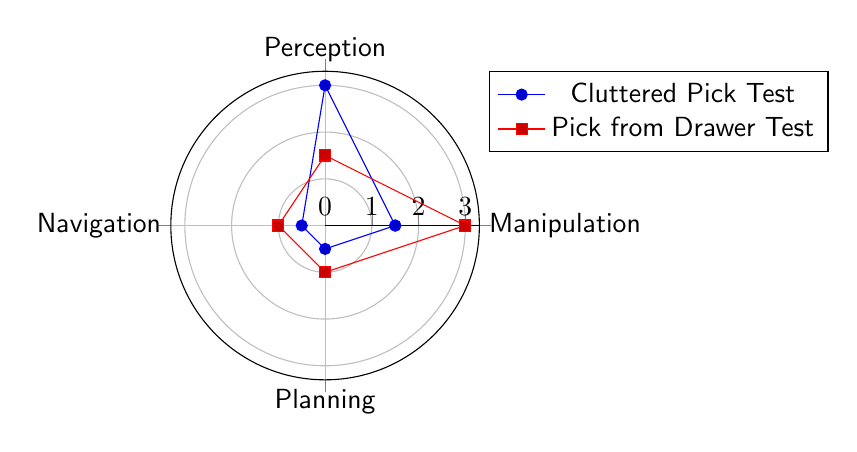
\begin{tikzpicture}
  	\begin{polaraxis}[
        xtick ={0, 90, 180, 270},
        xticklabels= {Manipulation, Perception, Navigation, Planning},
        width=5.5cm,
        height=5.5cm,
        legend pos=outer north east,
    ]
  	\addplot
  		coordinates {(0,1.5) (90,3) (180, 0.5) (270,0.5) (0, 1.5)};  % cp
      \addlegendentry{Cluttered Pick Test}
    \addplot
    	coordinates {(0,3) (90,1.5) (180,1) (270,1) (0,3)};  % pfd
      \addlegendentry{Pick from Drawer Test}
  	\end{polaraxis}
  \end{tikzpicture}
  \label{Examplary Challenge introducing a long term operation based on an extended Final test}
\end{figure}

The challenges of 2021 focussing on perception and manipuation in two scenarios. While "Cluttered Pick Test" (CP) adresses the robustness of perception, the "Pick from Drawer Test" (PFD) is focused on additional complexity by including objects in a drawer. Additonally, the start of a league specific simulator, to ease entry of new teams and enable better scientific evaluation is to be established through Simulation Evaluation Test (SE).

\end{comment}

% !TEX root = ../Rulebook.tex

\newpage
\subsection{Master Communication Test}

The purpose of the \iaterm{Master Communication Test}{MCT} is to introduce the atwork-commander to all (espeically new) teams and encourage them to implement reliable communications.
Therefore, a BTT1 test configuration is created but not sent as whole, but rather as individual transportation tasks.
Robots must confirm a successfully completet task before receiving the next one, meaning they can only perform one task if they do not have logging / feedback implemented.

%% !TEX root = ../Rulebook.tex

\section{Real Object Test}

The purpose of the \iaterm{Real Object Test}{ROT} is to introduce a new set of objects to the league that aims to replace the hard-to-get RoCKin objects.

Therefore, a BTT2 test configuration is created that only includes the new objects defined in section \ref{sec:new_objects}. Teams should be able to participate if they are able to detect and grasp the new objects.

% !TEX root = ../Rulebook.tex

\subsection{Coworker Assembly Test}

In the \iaterm{Coworker Assembly Test}{COT}, 
the goal is for a robot to produce a product while cooperating with a human worker.

Therefore, the robot has to collect three components scattered in the arena and bring them to a single workstation where the human worker waits on the other side of the table.
The robot has to place the objects and then wait for the human to assemble the objects to a product.
Once the human worker (a teammember of the performing team) has assembled the product, he/she must place the product back onto the table and give the robot a completion signal. This may be done via sign (visual) or voice (acoustic). It is not allowed to use controller or keyboard input.

Once the robot has recognized the signal, 
it must detect the assembled product, grasp it and then deliver it to another workstation.
This step concludes the assembly process by imitating the transport of the product to a warehouse.

Three object sets can be assembled during the COT: 
\begin{itemize}
	\item Set 1: Screw M20\_100 and Spacer and Nut M20
	\item Set 2: Bearing2 and  Housing
	\item Set 3: Axis2 and Nut M20  
\end{itemize}

%\newpage
\section{RoboCup Manipulation Challenge}

This challenge is not part of the normal @work technical challenges, but because it's about manipulation, all @Work-Teams are invited to participate. It's a joint challenge between RoboCup@Home and RoboCup@Work on
Autonomous Robot Manipulation (ARM), supported by MathWorks. More details can be found  at \url{arm.robocup.org}.

All teams which are already registered for @Work (or @Home) can participate (or register for the challenge only). All participants will receive a certificate of participation and all teams which delivers a working solution with non-zero performance will receive a \grqq proficiency\grqq \ certificate on robot manipulation and MathWorks tools issued by RoboCup Federation and MathWorks. The winner will receive an award of up to \$5,000 in the form of a grant for research acitivities. This challenge will continue and envolve in the next years.

\chapter{Challenges and Awards} \label{cha:ChallengesAndAwards}
\label{cha: CAA}
% !TEX root = ../Rulebook.tex

\section{Technical Challenges}
% !TEX root = ../Rulebook.tex

In the medium term, the \RCAW aims to transfer specific aspects of industrial scenarios in the tests and to demonstrate the practical applicability of the solutions. The challenges, which are adapted or redefined annually, serve as a test platform for the further development of the competitions. Each technical challenge is separately awarded. That means, teams can participate in any number of them. Hoewever any challenge will only be awarded if at least two teams competed unless the only competing team provided an outstanding performance.

A challenge increases the level capabilities of a robot in \RCAW related to:

\begin{itemize}
  \item \textbf{Variability of the environmental conditions} ... The setup conditions of a run are designed variably including disturbances. The lighting situations in the arena are changed dynamically, the configuration of the tables (height, format) is adapted or manipulation objects are mixed with unknown decoy objects.
  \item \textbf{Complexity of the scenarios} ... New arena elements are involved in a scenario
  or its dimensions (size, duration) are increased. This includes, for example, multi-robot scenarios, assembly tasks or new interaction stations.
\end{itemize}

For a successful implementation either an existing solution has to be increased in robustness or a new approach for an additional task has to be developed. The challenges here lie in the fields of perception, manipulation, navigation and planning.

This years challenges try to introduce the relatively new atwork-commander and the planned set of new objects (see \ref{sec:new_objects}).
These changes seem highly important for the participation of new teams, which is why we encourage every team to participate in atleast one technical challenge.

The exact test definition is still missing at the moment, but as the challenges are not part of the main scoring system, some of the rules may be adjusted to the requirements of the teams.

\begin{comment}
\begin{figure}[h!]
  \centering
  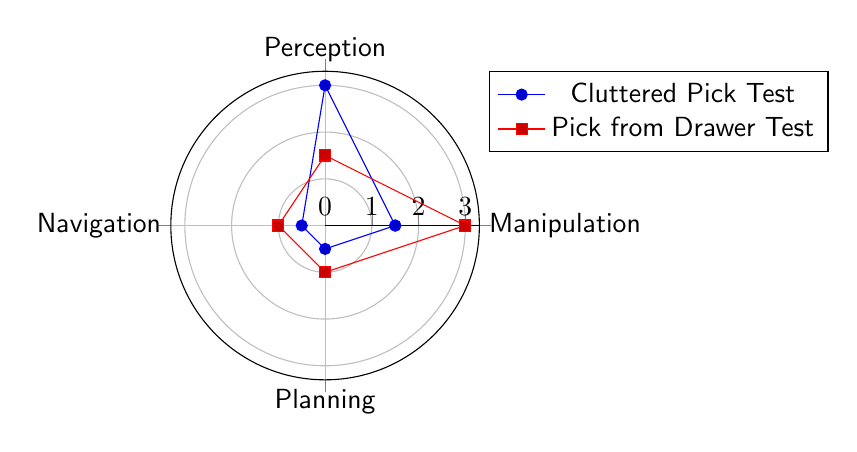
\begin{tikzpicture}
  	\begin{polaraxis}[
        xtick ={0, 90, 180, 270},
        xticklabels= {Manipulation, Perception, Navigation, Planning},
        width=5.5cm,
        height=5.5cm,
        legend pos=outer north east,
    ]
  	\addplot
  		coordinates {(0,1.5) (90,3) (180, 0.5) (270,0.5) (0, 1.5)};  % cp
      \addlegendentry{Cluttered Pick Test}
    \addplot
    	coordinates {(0,3) (90,1.5) (180,1) (270,1) (0,3)};  % pfd
      \addlegendentry{Pick from Drawer Test}
  	\end{polaraxis}
  \end{tikzpicture}
  \label{Examplary Challenge introducing a long term operation based on an extended Final test}
\end{figure}

The challenges of 2021 focussing on perception and manipuation in two scenarios. While "Cluttered Pick Test" (CP) adresses the robustness of perception, the "Pick from Drawer Test" (PFD) is focused on additional complexity by including objects in a drawer. Additonally, the start of a league specific simulator, to ease entry of new teams and enable better scientific evaluation is to be established through Simulation Evaluation Test (SE).

\end{comment}

% !TEX root = ../Rulebook.tex

\newpage
\subsection{Master Communication Test}

The purpose of the \iaterm{Master Communication Test}{MCT} is to introduce the atwork-commander to all (espeically new) teams and encourage them to implement reliable communications.
Therefore, a BTT1 test configuration is created but not sent as whole, but rather as individual transportation tasks.
Robots must confirm a successfully completet task before receiving the next one, meaning they can only perform one task if they do not have logging / feedback implemented.

%% !TEX root = ../Rulebook.tex

\section{Real Object Test}

The purpose of the \iaterm{Real Object Test}{ROT} is to introduce a new set of objects to the league that aims to replace the hard-to-get RoCKin objects.

Therefore, a BTT2 test configuration is created that only includes the new objects defined in section \ref{sec:new_objects}. Teams should be able to participate if they are able to detect and grasp the new objects.

% !TEX root = ../Rulebook.tex

\subsection{Coworker Assembly Test}

In the \iaterm{Coworker Assembly Test}{COT}, 
the goal is for a robot to produce a product while cooperating with a human worker.

Therefore, the robot has to collect three components scattered in the arena and bring them to a single workstation where the human worker waits on the other side of the table.
The robot has to place the objects and then wait for the human to assemble the objects to a product.
Once the human worker (a teammember of the performing team) has assembled the product, he/she must place the product back onto the table and give the robot a completion signal. This may be done via sign (visual) or voice (acoustic). It is not allowed to use controller or keyboard input.

Once the robot has recognized the signal, 
it must detect the assembled product, grasp it and then deliver it to another workstation.
This step concludes the assembly process by imitating the transport of the product to a warehouse.

Three object sets can be assembled during the COT: 
\begin{itemize}
	\item Set 1: Screw M20\_100 and Spacer and Nut M20
	\item Set 2: Bearing2 and  Housing
	\item Set 3: Axis2 and Nut M20  
\end{itemize}

%\newpage
\section{RoboCup Manipulation Challenge}

This challenge is not part of the normal @work technical challenges, but because it's about manipulation, all @Work-Teams are invited to participate. It's a joint challenge between RoboCup@Home and RoboCup@Work on
Autonomous Robot Manipulation (ARM), supported by MathWorks. More details can be found  at \url{arm.robocup.org}.

All teams which are already registered for @Work (or @Home) can participate (or register for the challenge only). All participants will receive a certificate of participation and all teams which delivers a working solution with non-zero performance will receive a \grqq proficiency\grqq \ certificate on robot manipulation and MathWorks tools issued by RoboCup Federation and MathWorks. The winner will receive an award of up to \$5,000 in the form of a grant for research acitivities. This challenge will continue and envolve in the next years.

\section{Open Source Award}
\label{sec: osa}
% !TEX root = ../Rulebook.tex

% \section{Open Source Award}

The \iaterm{Open Source Award}{OSA} can be given to a team that contributes part of its hardware architecture or software.
The open source solution to a specific problem can be used by other teams (especially new ones) as a starting point for their own development.
This contributes to the ongoing development and research of the league.

Teams can apply for the award on-site at a RoboCup@Work competition.
Links to the open source resources, including sufficient documentation, must be provided.
All participating teams review and rate the material internally and communicate their decision to the TC via the team leader.
The TC is not involved in the evaluation process.

Voting criteria may include
\begin{itemize}
	\item Usefulness
	\item Well documented
	\item Complexity
	\item Easily adaptable by other teams
\end{itemize}

\textbf{Voting System}: Each participating team will receive a score from 0-5. 
0 points would mean that no meaningful material is provided. 
5 points would mean that the submitted material fully meets the team's voting criteria.
The TC adds up the votes. The team with the most points wins the OSA \textbf{if the number of points divided by the number of voting teams is at least 3}.

\chapter{Virtual RoboCup}
\label{cha: VRC}
% !TEX root = ../Rulebook.tex

\section{General} 
\label{sec:VRCGeneral}

Since the start of the the Covid-19 pandemic, the RoboCups could not take place in person.
In 2021, the first virtual RoboCup was hosted online, requiring teams to livestream their robots performance in their own laboratory.
A ruleset was created that made a fair competition possible, which may be used for future online RoboCups.

Participating teams have to follow the guideline to provide an infrastructure that enables the TC and OC to evaluate their performance and to communicate during the competitions.
As the organization of such an online event is rather new for everyone and requires extended communication, 
every team should join the official \RCAW discord server (see \ref{ssec:LeagueInfrastructure}).
Announcements will be made via specific channels on this server.
Please participate in discussions and ask questions if you have any.

\section{Arena Setup} 
\label{sec:VRCArenaSetup}

As all teams will have different laboratory setups and some may not have the same resources (open space, workstations, etc.) as others, no fixed arena design will be used for a virtual \RCAW. We expect that this would either exclude some teams from the competitions or limit others in their test scenario design, which is why every team may design their own arena.

However, to ensure that the different robot performances can be compared using the existing scoring system (\ref{fig:test_specifications_instance}), some rules are defined to encourage teams to create challenging arena designs. In addition to the basic rules described in \ref{sec:ArenaDesign}, teams are required to consider: 
  
\begin{itemize}
\item The size of the Arena must be atleast 4m x 2m
\item The table placements should force the robot to move around the arena (not all the tables are next to each other)
\item Workstations should be accessible via multiple paths, so one of them may be blocked with obstacles (\ref{fig:vrc_arena_example} orange dots). Some space must be available for non-blocking obstacles (\ref{fig:vrc_arena_example} dark green dots).
\item Tables with the heights defined in (\ref{fig:test_specifications_instance}) have to be provided (margin = 2cm). If a team doesn't have enough workstations of one type for a test, the TC may allow alternative table heights to be used (especially BTT2, ATTs and Final). This rule does not apply for the Rotating Table, the Shelf and the Precise Placement station.
\item PPT cavities (a)-(f) (see \ref{fig:ppt_tiles}) must be provided. Teams may 3D print the cavities using the files in the leagues github. Standing objects are excluded. It must be possible to place ${N\_PLACE + 2}$ next to each other, so that atleast two decoy cavities can be used. 
\item Required arbitrary surfaces types: artificial grass, pvc floor / wood, mirror / aluminum foil, (plexi-)glass. 
These can be found in your local homedepot. (See fig. \ref{fig:vrc_obst_arbi}(b))
\item One path blocking and one small obstacle must be available both for physical objects and barriertape. (See fig. \ref{fig:vrc_obst_arbi}(a))
\end{itemize}

Figure~\ref{fig:vrc_arena_example} shows one possible example of an arena configuration in a small area.
Table heights are measured in cm. 
The orange dots mark possible path blockades, while the dark green lines mark optional obstacle placements. 


\begin{figure}[h!]
\centering
\includegraphics[width=0.9\textwidth ]{./images/vrc_arena_example.png}
\caption{Example Arena for a small VRC Setup --- Left: Annotated map - Right: Real Image }
\label{fig:vrc_arena_example}
\end{figure}

\begin{figure} [h!]
\begin{center}
\subfloat[Obstacle Placements]{\includegraphics[height = 5cm]{./images/vrc_obstacles.jpg}} \hspace{1cm}
\subfloat[Arbitrary Surfaces]{\includegraphics[height = 5cm]{./images/vrc_arbitrarys.jpg}}
\end{center}
\caption{Example obstacle placements and arbitrary surfaces}
\label{fig:vrc_obst_arbi}
\end{figure}

\section{Files required from Teams}

To enable the committee to generate fair tasks for every team, teams must provide detailed information about their arena and object inventory \textbf{1 month} prior to the first competition day. A zip-folder containing the following data must be sent via our discord server:

\begin{itemize}
\item Atleast two images of the arena from different perspectives. If two cannot cover the whole arena, teams must provide as many as needed.
\item A map of the arena with workstations marked (name + height). Teams may use an RVIZ screenshot containing the grid (1m cell size) and the occupancy grid (your map), which may be annotated using e.g. gimp (see also \ref{fig:vrc_arena_example}).
\item A list of available workstations in their arena (height and amount).
\item Images of the available arbitrary surfaces
\item Images of the available barriertape and obstacles
\item A list of available objects and containers (amount)
\item Image of the objects and containers
\item Images of the robot (all sides)
\item Robot dimensions in meter
\item Which tests the team intends to participate in
\item atWork-commande launchfiles
\end{itemize}

The folder must be named VRC-YEAR-info-TEAM-NAME and shall contain the subfolders ARENA, OBSTACLES, OBJECT, ROBOT, TESTS, REFBOX. 
File names must contain information about the data (e.g. Arena-Image-1) and must not have default names (e.g. IMG2012).

\section{Qualification for the competitions}

The TC will decide if the individual arenas qualify for the tests defined in \ref{fig:test_specifications_instance}. 
The main requirements are already specified in \ref{sec:VRCArenaSetup}, while the table describes individual task requirements more precisely.
 
If an arena does not qualify, the TC must notify the team \textbf{3 weeks} before competition starts, 
briefing the team about shortcomings and possible solutions. 
The team then has \textbf{1 week} to follow the TCs advice and provide a new zip-folder.
If an arena does not qualify for a test, the TC may decide to exclude the associated team from those.
If an arena only partly qualifies (e.g. no barriertape available), score adjustments can be made.


\section{Camera Setup} 
\label{sec:VRCCameraSetup}

Since the referees are not present at the arena during the Virtual RoboCup, the arena and all activities of the robot must be shown via livestream. For this purpose, cameras must be able to monitor the entire arena for the referees and the cameras should be mounted at least at head height. No blind spots are allowed when streaming the arena, so that the referees can see and evaluate every activity of the robot. Furthermore, the PC used to start the runs should also be monitored with the cameras so that the referees can observe every interaction with the PC. One or more cameras can be used to stream the arena. The OC will announce the streaming software used and the maximum number of livestreams available before the competition.
\par
In addition to the cameras for the arena, there must be a person who follows the robot with a mobile camera and shows the robot's activities from close up. This allows the referees to detect even small mistakes. The person is allowed to enter the arena during the run. However, the person is not allowed to interact with the robot.
\par
A camera may also be attached to the robot to better show the robot's activities to the referees and spectators. The camera on the robot is optional.

%\section{RoCKIn manipulation object set} 
%\label{sec:VRCRoCKInSet}
%The RoCKIn objects (see table \ref{tab:manipulation_objects_rockin}) are no longer produced and sold. Because of this, it is allowed to create these objects with a 3D printer at the Virtual RoboCup. However, the 3D printed RoCKIn objects must not be mixed with original objects. This means that the complete RoCKIn object set is either original or 3D printed. Furthermore, the 3D printed objects must have the same color. This applies only to the RoCKIn object set and not to the RoboCup@Work object set (see table \ref{tab:manipulation_objects}). The RoboCup@Work object set must not be 3D printed.


\section{Task Generation} 
\label{sec:VRCTaskGen}

The new atWork-commander implementation, which can be found here (https://github.com/robocup-at-work/atwork-commander), 
gives great opportunity to generate individual tasks for every participating team.

We advise all teams to use and test the new Atwork Commander. Teams must send configuration files for the new Atwork Commander with their arena design, so that the TC/OC can generate tasks for their arena. The config file for the arena shall contain the workstation names and heights and the available objects for a team. Teams may contact the committee via Discord if they face problems with this.  

As normally the atWork-commander would be provided by the OC onsite, no actual atWork-commander will be used during the online competition.
The OC will create the tasks for the tests using the official atWork-commander and the parameters provided by the teams. 
For each test, a single bagfile (10s) will be recorded which contains all topics published by the atwork\_commander.

Teams must be able to play a bagfile on an external computer, which is connected to the robot via WiFi.
The bagfile then must be played to start a competition. The robot should receive the task and start with the execution phase.

To prevent incompatible bagfiles during the competition, 
the OC will provide test bagfiles \textbf{2 weeks} before official competitions begin.
The working parameter and launchfiles will be saved and used to generate the specific task bagfiles for the competition.

\section{Competition Test Procedure} 
\label{sec:VRCTestExec}

\subsection{Preparation} 

Before a test begins, the OC will announce obstacle placements, object positions and arbitrary surface application to a team \textbf{10 minutes} prior to their timeslot. Teams must prepare the arena accordingly. The task bagfile will be sent out to the team \textbf{5 minutes} before their official timeslot. Note: The durations may be modified during the competitions if they show to be unsuitable.

\subsection{Test Start} 

The OC may count down before a competition (3, 2, 1, go), after which they start a timer according to the test durations in \ref{fig:test_specifications_instance}. On GO command, the active team may access the keyboard of the remote pc \textbf{only} to start the bagfile. The cameraman/-woman must show that to the audience.

\subsection{Test Run} 

The audience and especially the refs watch the livestream and rate the performance. In case of a major collision or any other reason for a restart, the remote pc keyboard may be accessed to restart the robot and the bagfile. The replay of the bagfile command must be shown to the audience once again, and afterwards the keybord must not be used anymore.

\subsection{Test End} 

The run ends when the timer is up, with an optional margin of five seconds due to the possible network delay. The refs then gather and discuss their performance evaluation.  

\section{Scoring} 
\label{sec:VRCScoring}

The different arena setups make time bonuses unfair and therefore they wont be awarded. 
The rest of the scoring will be the same as in a normal robocup scenario, with score/runtime adjustments and/or penalty points possible to compensate for missing test elements (see \ref{sec:VRCArenaSetup}). Such adjustments could be:

\begin{itemize}
\item The runtime for a test may be reduced if the arena is very small
\item If no barriertape is available, all penalty points for crossing will be applied
\item If no arbitrary surface is available, the object to pick will also be removed. 
\item No containers = no placement points given
\end{itemize}

Depending on the arena setups of all teams, these rules will be defined more precisely before the competitions begin.

\section{Technical Challenges} 
\label{sec:VRCTecCha}

A virtual robocup will focus on the main competition. No technical challenges will be performed during the official competitions. As some teams still requested technical challenges, we accept submissions by video. 
This is because that we expect a relatively tight schedule due to the different time zones of the teams and we are unsure if the technical challenges may be performed otherwise.

As the challenges do not count into the official scoring, teams are allowed to modify their arena. They still must stick to the rules defined in \ref{cha: TCHA}. The bagfile for the specific challenge will be sent out to the teams on the first day of the competitions. Teams are required to record a video of their challenge with a camera setup similar to \ref{sec:VRCCameraSetup}, which must be cut in a way that it is possible to see every region of interest (robot, no operator on pc, arena) at all times. The video must be rendered to mp4 format and uploaded to a cloud (e.g. onedrive). 
Teams must provide a link to their video via our discord server with the deadline set to last competition day, more specificly the beginning of the final runs.

The committee will review all submissions and rate the individual performances with the help of the referee team after the finals have been completed. Videos that exceed the deadline will not be reviewed and the teams participation in the challenge will be cancelled.















%\chapter{Future Changes}
%\label{cha: Future}
%% !TEX root = ../Rulebook.tex

\section{New Objects} 
\label{sec:new_objects}

In the year 2023 there will be new objects introduced to the rulebook this is due to the fact that the RockIn Objects (see Table~\ref{tab:manipulation_objects_rockin}) are no longer sold and available. The RoCKIn Objects and the R20 will be removed from the object set and the following new standardised mechatronic objects will be introduced (see Table~\ref{tab:new_objects} )

\begin{table}[h!]
	\begin{tabular}{|m{2cm}|c|c|m{8cm}|}
		\hline
		Object & Symbolic Description & Mass & Details \\
		\hline
%%%%%%%%%%%%%
		\imageView{./images/newObjects/welle3d.jpg} \newline
		\imageView{./images/newObjects/welleSchematic.JPG}
		& \texttt{Axis2} & 180 g & Steel axis \newline
		Misumi: SFUB25-25-F28-P17-T15-S10-Q20 \newline
		Coating/Colour: blank, black burnished \newline
		Length: 68 mm \newline
		Diameter: 17mm, M20 \newline
		see Figure~\ref{fig:welle2Schematic} \newline
		\href{https://de.misumi-ec.com/vona2/detail/110302635710/?CategorySpec=00000146753%3a%3ab%2cc}{Misumi} (visited Januar 2022)\\
			\hline
%%%%%%%%%%%%
		\imageView{./images/newObjects/bearing2.JPG} & \texttt{Bearing2} & 100 g & Bearing \newline 
		SKF YAR203-2F\newline
		Coating/Colour: gray \newline
		Useable with housing\newline
		\href{https://www.skf.com/sg/products/rolling-bearings/ball-bearings/insert-bearings/productid-YAR%20203-2F}{SKF}  (visited Januar 2022)\\
		\hline
%%%%%%%%%%%%				
		\imageView{./images/newObjects/housing.JPG} & \texttt{Housing} & 60 g & Housing \newline 
		SKF P40\newline
		Coating/Colour: gray \newline
		Useable with bearing\newline
		\textbf{Remark:} needs two hex socket screw M8x10 (DIN EN ISO 4762, DIN 912, CSN 021143, PN 82302, UNI 5931) and two M8 nuts (ISO 4032, DIN 934) \newline
		\href{https://www.skf.com/sg/products/mounted-bearings/ball-bearing-units/pillow-block-ball-bearing-units/productid-P%2040}{SKF}  (visited Januar 2022)\\
		\hline
%%%%%%%%%%%%	
		\imageView{./images/newObjects/motor.JPG} & \texttt{Motor2} & 350g & Motor 755\newline
		Coating/Colour: gray \newline
		Size: $66.7 \times 42.0 \si{\milli\meter}$\newline
		Diameter: $d_{axis}=5\si{\milli\meter}$, $l_{axis}=10\si{\milli\meter}$ \newline
		\href{https://www.amazon.de/EsportsMJJ-12V-36V-3500-9000Rpm-Drehmoment-Hochleistungsmotor/dp/B075D85KVV}{Amazon}  (visited Januar 2022)\\
		\hline
%%%%%%%%%%%%					
		\imageView{./images/newObjects/FlangedResinCollar.JPG} & \texttt{Spacer} &  & Flanged Spacer\newline
		Misumi CLJHJ25-30-70  \newline
		Coating/Colour: white \newline
		Size: $70\si{\milli\meter}$\newline
		Diameter: $d_{inner}=25\si{\milli\meter}$, $d_{outer}=30\si{\milli\meter}$ \newline
		\href{https://us.misumi-ec.com/vona2/detail/110300236450/?curSearch=%7b%22field%22%3a%22%40search%22%2c%22seriesCode%22%3a%22110300236450%22%2c%22innerCode%22%3a%22%22%2c%22sort%22%3a1%2c%22specSortFlag%22%3a0%2c%22allSpecFlag%22%3a0%2c%22page%22%3a1%2c%22pageSize%22%3a%2260%22%2c%2200000042362%22%3a%22mig00000001500952%22%2c%2200000042368%22%3a%22b%22%2c%22jp000157843%22%3a%22mig00000000344081%22%2c%22jp000157846%22%3a%22mig00000001417174%22%2c%22jp000157851%22%3a%22mig00000000344088%22%2c%2200000334029%22%3a%2230%22%2c%2200000334032%22%3a%2270%22%2c%22typeCode%22%3a%22CLJHJ%22%2c%22fixedInfo%22%3a%22MDM0000085422111030023645020110476153310093415426696895%7c14%22%7d&Tab=preview}{Misumi}  (visited Januar 2022)\\
						\hline

\end{tabular}
\caption{\RCAW New set of manipulation objects (components set).}
\label{tab:new_objects1}
\end{table}


\begin{table}[h!]
	\begin{tabular}{|m{2cm}|c|c|m{8cm}|}
		\hline
		Object & Symbolic Description & Mass & Details \\
		\hline
		%%%%%%%%%%%%
		\imageView{./images/newObjects/weraScrewdriver.jpg} & \texttt{Screwdriver } & 19g & WERA 352 \newline
		Ball end screwdriver,hexagon socket screws\newline
		Coating/Colour: black/green \newline
		Size: $181\si{\milli\meter}$\newline
		Diameter: $d_{tip}=2.5\si{\milli\meter}$\newline
		Code: 05138070001\newline
		\href{https://www.amazon.de/Wera-05138070001-352-Sechskant-Kugelkopf-Schraubendreher-2-5/dp/B00154ZWFI?th=1}{Amazon}  (visited Januar 2022)\\
		\hline
		%%%%%%%%%%%%			
		\imageView{./images/newObjects/weraWrench.jpg} & \texttt{Wrench } & ca. 72g & WERA Jocker 6000, 8mm \newline
		Ratcheting combination wrenches\newline
		Coating/Colour: silver/grey/pink \newline
		Size: ca. $144\si{\milli\meter}$\newline
		Diameter: $d_{max}=20\si{\milli\meter}$\newline
		Code: 05073268001\newline
		\href{https://www.amazon.de/Wera-05073268001-Joker-Maul-Ringratschen-Schl%C3%BCssel/dp/B00BT0GBMG?th=1}{Amazon} (visited Januar 2022)\\
		\hline
		%%%%%%%%%%%%
		\imageView{./images/newObjects/hsscoDIN338metaldrill.jpg} & \texttt{Drill } & ca. 10g & Bosch Drill HSS-Co DIN338  \newline
		Drill\newline
		Coating/Colour: gold/ Cobalt alloy \newline
		Length: ca. $151\si{\milli\meter}$\newline
		Diameter: $d_{max}=13\si{\milli\meter}$\newline
		Code: 3165140382724 \newline
		\href{https://www.amazon.com/Bosch-2609255086-Metal-Drill-HSS-Co/dp/B0071OSFQY}{Amazon} (visited Januar 2022)\\
		\hline
		%%%%%%%%%%%
		\imageView{./images/newObjects/weraAllenKey.jpg} & \texttt{AllenKey } & ca. 10g & Wera Allen Key 8mm,\newline
		3950 PKL L-key, metric, stainless\newline
		Coating/Colour: silver \newline
		Length: ca. $195\si{\milli\meter} \times 37\si{\milli\meter}$\newline
		Diameter: $d_{max}=8\si{\milli\meter}$\newline
		Code: 05022708001 \newline
		\href{https://www.amazon.co.uk/Wera-WER022708-Hexagon-Keys-Multi-Colour/dp/B00A8QXTNG}{Amazon} (visited Januar 2022)\\
		\hline
		%%%%%%%%%%%
	
\end{tabular}
\caption{\RCAW New set of manipulation objects (tool set).}
\label{tab:new_objects2}
\end{table}

			
\begin{figure}[h!]
	\begin{center}
		\includegraphics[width=\textwidth]{./images/newObjects/welleSchematic.JPG}
	\end{center}
	\caption{Schematic drawing of new manipulation object Axis2. Made of steel, blank or black burnished.}
	\label{fig:welle2Schematic}
\end{figure}

%\chapter{Open Source Award}
%\section{Introduction and Motivation}

In order to foster the development of new teams and to increase cooperation among established teams, the league announces an Open Source Award. As demonstrated
in other \RC major leagues, releasing software and/or hardware as open source fosters the overall progress of the league. Similarly, to other open source awards in \RC, all institutions, persons and teams who took part in national and international \RCAW competitions in \YEAR or the previous year are eligible to participate.

\section{Application}
The application should contain the following items:

\begin{itemize}
	\item A technical report and description (max. 8 pages in Springer LNCS style) about the open source artifact (software/hardware or both). The report should briefly describe the open source project objectives, design decisions and most importantly should exemplify it's importance for the \RCAW competition and community.
	\item A online reference, documentation, tutorial (e.g. website, Github page etc.) for the presented open source material. This includes also statements about licensing (e.g. which kind of open source license such as GPL, LGPL, Apache, etc.) and usage.
\end{itemize}

\all{update the application deadline:}
Application deadline is the: 01.05.2016. Application material needs to be send via email to: \texttt{rc-work-tc@lists.robocup.org}. Please note, in case the evaluation committee receives  only applications which do not fulfill the desired level of quality, the award will not be given in \YEAR. The winner(s) will be announced during the RoboCup \YEAR award ceremony.


\section{Evaluation}
Evaluation is performed by an external jury chosen by the EC and TC. The evaluation criteria are the following:

\begin{itemize}
	\item Relevance: \emph{Is the presented material relevant for \RCAW? Can the material be applied in the context of \RCAW?}
	\item Originality: \emph{Does the presented material solve a problem/issue in \RCAW in a very appealing, general approach?}
	\item Technical Quality: \emph{Is the presented material well-designed and well-developed. This also includes coding style etc.? }
	\item Presentation: \emph{Is the presentation of the material appealing and complete for \RCAW purpose?}
\end{itemize}


%\newpage
\section{Basic Welding Test}

\subsection{Purpose and Focus of the Test}
The purpose of the \iaterm{Basic Welding Test}{BWT} is to demonstrate basic welding capabilities, like detecting a marker and performing spot welding. 
\par
The focus lies on the precision needed in many welding scenarios. After detecting the target, the target needs to be reached closely and than a laser pointer should be activated for an pre defined amount of time.

\subsection{Scenario Environment}
The arena used for this test contains basically all elements as for the Basic Navigation Test. Additionally to environmental elements (walls, service areas, floor markers, etc.), an object with spot markers (see Fig. \ref{BWT_Label}) will be added on one or more service areas. 

\begin{figure} [h!]
\begin{center}
\includegraphics[width=\textwidth/4]{./images/BWT_Marker.jpg} 
\caption{The Marker used to identify the welding spots. The Blue areas are not specified and may be of any color. The middle part is the spot where the welding shall be performed.}
\label{BWT_Label}
\end{center}
\end{figure}


\subsection{Task}
A single robot is used. The robot starts at the defined start position outside the arena. The task consists of a sequence of spot welding operations. The objective is to successfully reach all spot markers and perform the spot welding operation. The task is finished once all spot markers are welded ant the robot has exited through the designated exit.
\par
The task specification consists of: 
\begin{itemize}
	\item The specification of the welding place or places (e.g. D0, S5, U2)
	\item The number of makers (1, 2, 3)
	\item The specification of a final place for the robot.
\end{itemize}

Two examples for a full task specification is as follows:
\begin{itemize}
	\item BWT\textless S1(2),S6(1),S7\textgreater 
\end{itemize}


\subsection{Complexity Options}

So far no complexity objections exist.

\subsection{Rules}
The following rules have to be obeyed:

\begin{itemize}
\item The order in which the teams have to perform will be determined by a draw.
\item A team has a time period defined int the instance specification.
\item At the beginning of a team's period, the team will get the task specification. 
\item The team must start at in the designated start area.
\item The laser used for the test must be of or below class 1 (according to IEC 60825)
\item The Spot is successfully welded if the robot has reached the spot and performed a welding operation for 3 seconds.
\item A Welding spot is reached when the laser of the robot when activated hits the spot and the distance between either the laser of an arbitrary extension of the laser is closer then 2 cm.
\end{itemize}


\subsection{Scoring}
Points are awarded as follows:

\begin{itemize}
\item 100 points are awarded for successfully performing a spot welding operation on a correct target.
\item - 100 points are awarded for performing the welding operation or activating the laser pointer in any location other then a specified marker.

\end{itemize}



%\newpage
\section{Advanced Welding Test}

\subsection{Purpose and Focus of the Test}
The purpose of the \iaterm{Advanced Welding Test}{AWT} is to welding in two Dimensions. 
\par
The focus is on the precision required to perform a correct welding task. The detection of where to weld and the correct motion following the line, while keeping a constant movement are the keys to a successful full completion of the task. 

\subsection{Scenario Environment}
The arena used for this test contains basically all elements as for the Basic Navigation Test. Additionally to environmental elements (walls, service areas, floor markers, etc.), an object with a contour on a flat surface (see Fig. \ref{awt_examplecontour}) will be added on one or more service areas. 

\begin{figure}
\begin{center}
\subfloat[]{\includegraphics[width = \textwidth/3]{./images/AWT_Corner.png}}
\subfloat[]{\includegraphics[width = \textwidth/3]{./images/AWT_Curve.png}} 
\subfloat[]{\includegraphics[width = \textwidth/3]{./images/AWT_Sinus.png}}  
\end{center}

\caption{Examples of Contours to be welded.}
\label{awt_examplecontour}
\end{figure}


\subsection{Task}
A single robot is used. The robot starts at the defined start position outside the arena. The task consists of navigating to the specified location and then welding along the defined contour. The task is finished once the contour is welded ant the robot has exited through the designated exit.
\par
The task specification consists of: 
\begin{itemize}
	\item The specification of the welding place or places (e.g. D0, S5)
	\item The specification of a final place for the robot.
\end{itemize}

Two examples for a full task specification is as follows:
\begin{itemize}
	\item AWT\textless S1,S7\textgreater 
\end{itemize}


\subsection{Complexity Options}

So far no complexity objections exist.

\subsection{Rules}
The following rules have to be obeyed:

\begin{itemize}
\item The order in which the teams have to perform will be determined by a draw.
\item A team has a time period defined int the instance specification.
\item At the beginning of a team's period, the team will get the task specification. 
\item The team must start at in the designated start area.
\item The laser used for the test must be of or below class 1 (according to IEC 60825)
\end{itemize}


\subsection{Scoring}
Points are awarded as follows:

A System will be introduced by the TC, that allows for Measuring the distance between the contour and the welded path. If the System allows for measuring the time spent at each part and the amount of attempts used they although can be scored. All points which are closer to a point on the counter then one cm count all correct, all other points are incorrect.
\par
To allow for scoring the contour will be represented by points at corners every one cm.

\begin{itemize}
\item 5 points are awarded for every percent of the contour or contours successfully welded.
\item -100 points for every point (clustered with 1 cm diameter) outside of the contour

\end{itemize}



%\newpage
\section{Basic Assembly Test}
In order to foster the development of the league and expand towards more complicated domains, an assembly challenge will be held. The focus is to show new and challenging aspects of assembly which can be performed by small service robots.

\subsection{Purpose and Focus of the Test}
The purpose of the \iaterm{Basic Assembly Test}{BAT} is to demonstrate basic assembly capabilities by the robots, like combining objects, by fitting or attaching them together.
The focus is on the manipulation towards assembly, e.g. force fitting or the preparation of objects to be attached by e.g. external devices and machines. This can include holding an object in place for another robot, machine or human to assemble it.

\subsection{Scenario Environment}
The arena used for this test contains all elements as for the Basic Navigation Test. In addition to environmental elements (such as walls, service areas, floor markers, etc.), different manipulatable objects will be placed on the service areas. On top of the service area, a car model will be mounted and fixed, so that the robot will not be able to move the car (see Fig \ref{fig:BAT_car}). The axle will be red, the tire blue and the car model will be neither.

\begin{figure} [h!]
\centering
\includegraphics[width=0.8\textwidth ]{./images/BAT.png}
\caption{A example scene for the Basic Assembly Test. The actual car model may differ, but the wheels (\emph{blue}) need to be fitted onto the axes (\emph{red}).}
\label{fig:BAT_car}
\end{figure}


\subsection{Manipulation Objects}
The manipulation objects in this test may include the objects specified in Table, as they can still be inside of the arena and function as decoy objects. \ref{tab:manipulation_objects}.
The set of objects is extended by:

\begin{table}[p]
\begin{tabular}{|c|c|c|p{5cm}|}
\hline 
 & Symbolic Description & Mass & Details \\ 
\hline 
\includegraphics[width=3cm]{./images/BAT_Tire.png}  & T50 & 20 g & Radius: 50mm \newline
 Height: 34mm \\
\hline 
\end{tabular} 

\label{tab:bat_objects}
\caption{Examples of assembly objects}
\end{table}

All objects can be printed using a 3D-printer (e.g. axis and wheel), the car model is only for visualization purposes. All parts are available as STL files in the official \RCAW \emph{model} repository (see Section \ref{ssec:LeagueInfrastructure}).


\subsection{Task}
A single robot is used. The task consists of a sequence of assembly operations, with a small base movement in between. The objective is to collect a set of objects and perform an assembly option. The robot will be given instruction where to pick up the wheels and where to assemble them. The task is to fit the wheels onto the axes. The wheels and the axes need to be detected by the robot. A few wheels may be already assembled. Therefore it is necessary to detect where a wheel is still missing. The wheels designated for assembly will lie flat on the service areas.

\par
The task specification consists of: 
\begin{itemize}
	\item Location(s) of the wheels
	\item Location(s) where the assembly takes places
\end{itemize}

\subsection{Rules}
The following rules have to be obeyed:

\begin{itemize}
\item The order in which the teams have to perform will be determined by a draw.
\item At the beginning of a team's period, the team will get the task specification. 
\item The team must set-up the robot in the designated start area.
\item An assembly object counts as successfully assembled when it is attached to the correct object or is in place for the external device to perform the assembly.
\item An assembly objects counts as assembled wrong when it is assembled wrong (e.g. fitting a second tire on one axle)
\item The maximum time and the number of assemblies to be performed will be determined during the event by the TC.
\end{itemize}


\subsection{Scoring}
Points are awarded as follows:

\begin{itemize}
\item correct assembly:  \hfill 100 points
\item wrong assembly:  \hfill -100 points
\end{itemize}




\renewcommand{\glsnamefont}[1]{\textbf{#1}}
%\setlength{\glslistdottedwidth}{.3\linewidth}
\glsaddall
%\printglossary[style=long, title=Special Terms]
%\printglossary[style=listdotted, title=Special Terms]
\printglossary[style=altlist, title=Special Terms]
\chapter{Appendix}
% !TEX root = ./Rulebook.tex

\section{Link list } 
\label{sec:new_objects}

Due to have a somehow standardised set of objects for each team. In Table~\ref{tab:shoppinglist} an example shopping list, including some links of different items needed is given.  

\begin{table}[h!]
\begin{tabular}{|m{2cm}|c|c|m{8cm}|}
\hline
Item & Symbolic Description & Shop & Details \\
\hline
Metal Axis& \texttt{Axis2} & Mitsumi & 	Misumi: SFUB25-25-F28-P17-T15-S10-Q20 \newline
\href{https://de.misumi-ec.com/vona2/detail/110302635710/?CategorySpec=00000146753%3a%3ab%2cc}{Misumi} (visited January 2022)\\
\hline
%%%%%%%%%%%%%
Bearing & \texttt{Bearing2} & SKF & SKF YAR203-2F\newline
\href{https://www.skf.com/sg/products/rolling-bearings/ball-bearings/insert-bearings/productid-YAR%20203-2F}{SKF}  (visited January 2022)\\
\hline
%%%%%%%%%%%%%
Bearing housing & \texttt{Housing} & SKF &  SKF P40\newline
\href{https://www.skf.com/sg/products/mounted-bearings/ball-bearing-units/pillow-block-ball-bearing-units/productid-P%2040}{SKF}  (visited January 2022)\\
\hline
%%%%%%%%%%%%
Motor & \texttt{Motor2} & Amazon& 	Motor 755\newline
\href{https://www.amazon.de/EsportsMJJ-12V-36V-3500-9000Rpm-Drehmoment-Hochleistungsmotor/dp/B075D85KVV}{Amazon}  (visited January 2022)\\
\hline
%%%%%%%%%%%%
Plastic Spacer & \texttt{Spacer} &  & Misumi CLJHJ25-30-70  \newline
\href{https://us.misumi-ec.com/vona2/detail/110300236450/?curSearch=%7b%22field%22%3a%22%40search%22%2c%22seriesCode%22%3a%22110300236450%22%2c%22innerCode%22%3a%22%22%2c%22sort%22%3a1%2c%22specSortFlag%22%3a0%2c%22allSpecFlag%22%3a0%2c%22page%22%3a1%2c%22pageSize%22%3a%2260%22%2c%2200000042362%22%3a%22mig00000001500952%22%2c%2200000042368%22%3a%22b%22%2c%22jp000157843%22%3a%22mig00000000344081%22%2c%22jp000157846%22%3a%22mig00000001417174%22%2c%22jp000157851%22%3a%22mig00000000344088%22%2c%2200000334029%22%3a%2230%22%2c%2200000334032%22%3a%2270%22%2c%22typeCode%22%3a%22CLJHJ%22%2c%22fixedInfo%22%3a%22MDM0000085422111030023645020110476153310093415426696895%7c14%22%7d&Tab=preview}{Misumi}  (visited Januar 2022)\\
\hline
%%%%%%%%%%%%
Screwdriver & \texttt{Screwdriver } & Amazon & WERA 352 \newline
Code: 05138070001\newline
\href{https://www.amazon.de/Wera-05138070001-352-Sechskant-Kugelkopf-Schraubendreher-2-5/dp/B00154ZWFI?th=1}{Amazon}  (visited January 2022)\\
\hline
%%%%%%%%%%%%%
Wrench & \texttt{Wrench } & Amazon & WERA Jocker 6000, 8mm \newline
Code: 05073268001\newline
\href{https://www.amazon.de/Wera-05073268001-Joker-Maul-Ringratschen-Schl%C3%BCssel/dp/B00BT0GBMG?th=1}{Amazon} (visited January 2022)\\
\hline
%%%%%%%%%%%%
Drill & \texttt{Drill } & Amazon &Bosch Metal Drill Bit HSS-Co 13 x 101 x 151 mm \newline
Code: 3165140382724\newline
\href{https://www.amazon.co.uk/Bosch-2609255086-Metal-Drill-HSS-Co/dp/B0071OSFQY/ref=sr_1_1?crid=1NW4BZK67OY63&keywords=bosch+3165140382724&qid=1642582541&s=diy&sprefix=bosch+3165140382724%2Cdiy%2C113&sr=1-1}{Amazon} (visited January 2022)\\
\hline
%%%%%%%%%%%%
AllenKey & \texttt{Allen Key } & Amazon & 3950 PKL L-key, metric, stainless, 8mm \newline
Code: 05022708001\newline
\href{https://www.amazon.co.uk/Wera-WER022708-Hexagon-Keys-Multi-Colour/dp/B00A8QXTNG}{Amazon} (visited January 2022)\\
\hline
%%%%%%%%%%%%
Containers & \texttt{Containers } & Amazon & Allit Box Size 2B \newline
\href{https://www.amazon.de/gp/product/B0062TUUOE/ref=ppx_yo_dt_b_asin_title_o01_s00?ie=UTF8&psc=1}{Amazon} (visited January 2022)\\
\hline
%%%%%%%%%%%%
Printing Material &  \texttt{PLA Material}& Amazon & Basic PLA filament \newline
\href{https://www.amazon.de/-/en/TINMORRY-1-75mm-Filament-Printer-Spool/dp/B089YX78N5/ref=sr_1_6?crid=ZTL2O0EL3B3B&keywords=pla%2Bfilament%2Bgrau%2Bral%2B9006&qid=1641982915&s=industrial&sprefix=pla%2Bfilament%2Bgrau%2Bral9006%2Cindustrial%2C114&sr=1-6&th=1}{Amazon} (visited Januar 2022) \\
\hline
%%%%%%%%%%%
\end{tabular}
\caption{Example shopping list of required items.}
\label{tab:shoppinglist}
\end{table}


\printabx
\printidx

\end{document}
